%% Dokumentenklasse (Koma Script) -----------------------------------------
\documentclass[%
  %draft,     % Entwurfsstadium
  final, % fertiges Dokument
  % --- Paper Settings ---
  paper=a4,paper=portrait, pagesize=auto, % [Todo: add alternatives]% landscape% driver
  % --- Base Font Size ---
  fontsize=11pt,%
  % --- Koma Script Version ---
  version=last, ]{scrreprt} %% Classes: scrartcl, scrreprt, scrbook

\usepackage{scrhack}

% Encoding der Dateien (sonst funktionieren Umlaute nicht)
% Fuer Linux -> utf8
% Fuer Windows, alte Linux Distributionen -> latin1

% Empfohlen latin1, da einige Pakete mit utf8 Zeichen nicht
% funktionieren, z.B: listings, soul.
%\usepackage[latin1]{inputenc}
%\usepackage[ansinew]{inputenc}
\usepackage[utf8]{inputenc}
\usepackage{xurl}
%\usepackage{ucs}
%\usepackage[utf8x]{inputenc}

%%%%%%%%%%%%%%%%%%%%%%%%%
%    SET LANGUAGE       %
%%%%%%%%%%%%%%%%%%%%%%%%%
\def\lang{ngerman} % Options: english or ngerman

% The used tool and the reason; remove command if it does not apply
\def\declareUseOfGenerativeAITool{ChatGPT~4}

%%% Preambel
%%% === Textbody ==============================================================
\KOMAoptions{%
   DIV=11,% (Size of Text Body, higher values = greater textbody)
   % DIV=calc % (also areaset/classic/current/default/last) 
   % -> after setting of spacing necessary!   
   BCOR=5mm}% (Bindekorrektur)%
%%% === Headings ==============================================================
\KOMAoptions{%
   %%%% headings
   % headings=small,  % Small Font Size, thin spacing above and below
   % headings=normal, % Medium Font Size, medium spacing above and below
   headings=big, % Big Font Size, large spacing above and below
   %
   headings=noappendixprefix, headings=nochapterprefix, % chapter in appendix as in body text% no prefix at chapters
   % headings=appendixprefix,   % inverse of 'noappendixprefix'
   % headings=chapterprefix,    % inverse of 'nochapterprefix'
   headings=openany, % Chapters start at any side
   % headings=openleft,  % Chapters start at left side
   % headings=openright, % Chapters start at right side      
   %%% Add/Dont/Auto Dot behind section numbers 
   %%% (see DUDEN as reference)
   % numbers=autoenddot
   % numbers=enddot
   numbers=noenddot
   % secnumdepth=3 % depth of sections numbering (???)
}%
\setcounter{secnumdepth}{3}
%%% === Page Layout ===========================================================
\KOMAoptions{% (most options are for package typearea)
   twoside=true, % two side layout (alternating margins, standard in books)
   % twoside=false, % single side layout 
   % twoside=semi,  % two side layout (non alternating margins!)
   %
   twocolumn=false, % (true)
   %
   headinclude=false,footinclude=false,mpinclude=false,%%%      
   %
   headlines=2.1,%
   % headheight=2em,%
   headsepline=true,footsepline=false,cleardoublepage=empty }%%%plain, headings%
%%% === Paragraph Separation ==================================================
\KOMAoptions{%
   % parskip=relative, % change indentation according to fontsize (recommanded)
   parskip=absolute, parskip=false % do not change indentation according to fontsize% indentation of 1em
   % parskip=true   % parksip of 1 line - with free space in last line of 1em
   % parskip=full-  % parksip of 1 line - no adjustment
   % parskip=full+  % parksip of 1 line - with free space in last line of 1/4
   % parskip=full*  % parksip of 1 line - with free space in last line of 1/3
   % parskip=half   % parksip of 1/2 line - with free space in last line of 1em
   % parskip=half-  % parksip of 1/2 line - no adjustment
   % parskip=half+  % parksip of 1/2 line - with free space in last line of 1/3
   % parskip=half*  % parksip of 1/2 line - with free space in last line of 1em
}%
%%% === Table of Contents =====================================================
\setcounter{tocdepth}{3} % Depth of TOC Display
\KOMAoptions{%
   %%% Setting of 'Style' and 'Content' of TOC
   % toc=left, %
   toc=indented,%
   %
   toc=bib,
   % toc=nobib,
   % toc=bibnumbered,
   %
   % toc=index,%
   toc=noindex,
   %
   % toc=listof,
   toc=nolistof
   % toc=listofnumbered,
   %   
}%  
%%% === Lists of figures, tables etc. =========================================
\KOMAoptions{%
   %%% Setting of 'Style' and 'Content' of Lists 
   %%% (figures, tables etc)
   % --- General List Style ---
   listof=left, listof=indented, % tabular styles% hierarchical style
   % --- chapter highlighting ---
   % listof=chapterentry, % ??? Chapter starts are marked in figure/table
   % listof=chaptergapline, % New chapter starts are marked by a gap 
   % of a single line
   listof=chaptergapsmall, % New chapter starts are marked by a gap 
   % of a smallsingle line
   % listof=nochaptergap, % No Gap between chapters
   %
   % listof=leveldown, % lists are moved one level down ???
   % --- Appearance of Lists in TOC
   % listof=notoc, % Lists are not part of the TOC
   listof=totoc % add Lists to TOC without number
   % listof=totocnumbered, % add Lists to TOC with number
}%  
%%% === Bibliography ==========================================================
%% Setting of 'Style' and 'Content' of Bibliography
\KOMAoptions{%
   % bibliography=oldstyle,%
   bibliography=openstyle,%
   % bibliography=nottotoc, % Bibliography is not part of the TOC
   % bibliography=totocnumbered, % add Bibliography to TOC with number
   bibliography=totoc }% add Bibliography to TOC without number%
%%% === Index =================================================================
%% Setting of 'Style' and 'Content' of Index in TOC
\KOMAoptions{%
   index=nottotoc % index is not part of the TOC
   % index=totoc, % add index to TOC without number
}%
%%% === Titlepage =============================================================
\KOMAoptions{%
   titlepage=true %
   %titlepage=false %
}%
%%% === Miscellaneous =========================================================
\KOMAoptions{% 	
   footnotes=multiple% nomultiple
   %open=any,%
   %open=left,%
   %open=right,%
   %chapterprefix=false,%
   %appendixprefix=false,%
   %chapteratlists=10pt,% entry
}%
% ------------------------------------------------------------------------
% LaTeX - Preambel  ******************************************************
% ------------------------------------------------------------------------
% von: Matthias Pospiech
% ========================================================================

% Strukturierung dieser Praeambel:
%    1.  Pakete die vor anderen geladen werden müssen
%        (calc, babel, xcolor, graphicx, amsmath, pst-pdf, ragged2e, ...)
%    2.  Schriften
%    3.  Mathematik (mathtools, fixmath, onlyamsmath, braket,
%        cancel, empheq, exscale, icomma, ...)
%    4.  Tabellen (booktabs, multirow, dcolumn, tabularx, ltxtable, supertabular)
%    5.  Text
%        5.1 Auszeichnungen (ulem, soul, url)
%        5.2 Fussnoten (footmisc)
%        5.3 Verweise (varioref)
%        5.4 Listen (enumitem, paralist, declist)
%    6.  Zitieren (csquotes, jurabib, natbib)
%    7.  PDF (microtype, hyperref, backref, hypcap, pdfpages
%    8.  Graphiken (float, flafter, placeins, subfig, wrapfig,
%        floatflt, picins, psfrag, sidecap, pict2e, curve2e)
%    9.  Sonstiges (makeidx, isodate, numprint, nomencl, acronym)
%    10. Verbatim (upquote, verbatim, fancyvrb, listings, examplep)
%    11. Wissenschaft (units)
%    12. Fancy Stuff
%    13. Layout
%       13.1.  Diverse Pakete und Einstellungen (multicol, ellipsis)
%       13.2.  Zeilenabstand (setspace)
%       13.3.  Seitenlayout (typearea, geometry)
%       13.4.  Farben
%       13.5.  Aussehen der URLS
%       13.6.  Kopf und Fusszeilen (scrlayer-scrpage)
%       13.7.  Fussnoten
%       13.8.  Schriften (Sections )
%       13.9.  UeberSchriften (Chapter und Sections) (titlesec, indentfirst)
%       13.10. Captions (Schrift, Aussehen)
%              (caption, subfig, capt-of, mcaption, tocloft, multitoc, minitoc)
%    14.  Auszufuehrende Befehle
%    15. DoDo Notes Package

% ~~~~~~~~~~~~~~~~~~~~~~~~~~~~~~~~~~~~~~~~~~~~~~~~~~~~~~~~~~~~~~~~~~~~~~~~
% Einige Pakete muessen unbedingt vor allen anderen geladen werden
% ~~~~~~~~~~~~~~~~~~~~~~~~~~~~~~~~~~~~~~~~~~~~~~~~~~~~~~~~~~~~~~~~~~~~~~~~

%%% Packages for LaTeX - programming
%
% Define commands that don't eat spaces.
\usepackage{xspace}
% IfThenElse
\usepackage{ifthen}
%%% Doc: ftp://tug.ctan.org/pub/tex-archive/macros/latex/contrib/oberdiek/ifpdf.sty
% command for testing for pdf-creation
\usepackage{ifpdf} %\ifpdf \else \fi

%%% Internal Commands: ----------------------------------------------
\makeatletter
%
\providecommand{\IfPackageLoaded}[2]{\@ifpackageloaded{#1}{#2}{}}
\providecommand{\IfPackageNotLoaded}[2]{\@ifpackageloaded{#1}{}{#2}}
\providecommand{\IfElsePackageLoaded}[3]{\@ifpackageloaded{#1}{#2}{#3}}
%
\newboolean{chapteravailable}%
\setboolean{chapteravailable}{false}%

\ifcsname chapter\endcsname
  \setboolean{chapteravailable}{true}%
\else
  \setboolean{chapteravailable}{false}%
\fi


\providecommand{\IfChapterDefined}[1]{\ifthenelse{\boolean{chapteravailable}}{#1}{}}%
\providecommand{\IfElseChapterDefined}[2]{\ifthenelse{\boolean{chapteravailable}}{#1}{#2}}%

\providecommand{\IfDefined}[2]{%
\ifcsname #1\endcsname
   #2 %
\else
     % do nothing
\fi
}

\providecommand{\IfElseDefined}[3]{%
\ifcsname #1\endcsname
   #2 %
\else
   #3 %
\fi
}

\providecommand{\IfElseUnDefined}[3]{%
\ifcsname #1\endcsname
   #3 %
\else
   #2 %
\fi
}


%
% Check for 'draft' mode - commands.
\newcommand{\IfNotDraft}[1]{\ifx\@draft\@undefined #1 \fi}
\newcommand{\IfNotDraftElse}[2]{\ifx\@draft\@undefined #1 \else #2 \fi}
\newcommand{\IfDraft}[1]{\ifx\@draft\@undefined \else #1 \fi}
%

% Definde frontmatter, mainmatter and backmatter if not defined
\@ifundefined{frontmatter}{%
   \newcommand{\frontmatter}{%
      %In Roemischen Buchstaben nummerieren (i, ii, iii)
      \pagenumbering{roman}
   }
}{}
\@ifundefined{mainmatter}{%
   % scrpage2 benoetigt den folgenden switch
   % wenn \mainmatter definiert ist.
   \newif\if@mainmatter\@mainmattertrue
   \newcommand{\mainmatter}{%
      % -- Seitennummerierung auf Arabische Zahlen zuruecksetzen (1,2,3)
      \pagenumbering{arabic}%
      \setcounter{page}{1}%
   }
}{}
\@ifundefined{backmatter}{%
   \newcommand{\backmatter}{
      %In Roemischen Buchstaben nummerieren (i, ii, iii)
      \pagenumbering{roman}
   }
}{}

% Pakete speichern die spaeter geladen werden sollen
\newcommand{\LoadPackagesNow}{}
\newcommand{\LoadPackageLater}[1]{%
   \g@addto@macro{\LoadPackagesNow}{%
      \usepackage{#1}%
   }%
}

\newcommand*{\printGenerativeAIDeclaration}{%
\ifcsdef{declareUseOfGenerativeAITool}{%
\ifthenelse{\equal{\lang}{ngerman}}%
{%
\section*{Erklärung zur Verwendung von generativer KI}
In Übereinstimmung mit den Empfehlungen der
Deutschen Forschungsgemeinschaft (DFG)\footnote{DFG formuliert Richtlinien für den Umgang mit generativen Modellen für Text- und Bild: \url{https://www.dfg.de/en/news/news-topics/announcements-proposals/2023/info-wissenschaft-23-72}}
und denen der Zeitschrift Theoretical Computer Science\footnote{Erklärung zur Verwendung von generativer KI in wissenschaftlichen Arbeiten: \url{https://www.sciencedirect.com/journal/theoretical-computer-science/publish/guide-for-authors}}
erkläre ich (der Autor/die Autorin) hiermit den Einsatz von generativer KI.

Bei der Vorbereitung dieser Arbeit habe ich 
\declareUseOfGenerativeAITool\ verwendet, um ausschließlich die Lesbarkeit und Sprache zu verbessern.
Nach der Verwendung von \declareUseOfGenerativeAITool\ habe ich 
den Inhalt überprüft und nach Bedarf bearbeitet und übernehme die volle Verantwortung 
für den Inhalt dieser Arbeit.
}
{%
\section*{Declaration of the use of Generative AI}
In accordance with the recommendation of 
the German Research Foundation (DFG - Deutsche Forschungsgemeinschaft)\footnote{DFG Formulates Guidelines for Dealing with Generative Models for Text and Image Creation: \url{https://www.dfg.de/en/news/news-topics/announcements-proposals/2023/info-wissenschaft-23-72}}
and that of the journal Theoretical Computer Science\footnote{Declaration of generative AI in scientific writing: \url{https://www.sciencedirect.com/journal/theoretical-computer-science/publish/guide-for-authors}}
I (the author) herby declare the use of generative AI.

During the preparation of this work I used 
\declareUseOfGenerativeAITool\ in order to improve readability and language, only.
After using \declareUseOfGenerativeAITool, I reviewed and edited 
the content as needed and take full responsibility 
for the content of this thesis.
}
}{}
}

\newcommand*\printDeclarationOfIndependence{%
\ifthenelse{\equal{\lang}{ngerman}}%
{%
\section*{Erklärung der Selbstständigkeit}
\thispagestyle{empty}
Hiermit versichere ich, die vorliegende Arbeit selbstständig verfasst und keine anderen als die angegebenen Quellen und Hilfsmittel benutzt sowie die Zitate deutlich kenntlich gemacht zu haben.
\vspace{4\baselineskip}\\
Gießen, den \today \hfill \theAuthor
\vspace{4\baselineskip}\\
}
{%
\section*{Declaration of Independence}
\thispagestyle{empty}
I hereby declare that I have composed the present work independently and have not used any sources or aids other than those cited, and that all quotations have been clearly indicated.
\vspace{4\baselineskip}\\
Gießen, on \today \hfill \theAuthor
\vspace{4\baselineskip}\\
}
}

\let\oldauthor\author
\renewcommand{\author}[1]{\oldauthor{#1}\newcommand{\theAuthor}{#1}}

\let\oldtitle\title
\renewcommand{\title}[1]{\oldtitle{#1}\newcommand{\theTitle}{#1}}

\newcommand*{\academicTitle}[1]{\newcommand{\theAcedemicTitle}{#1}}
\newcommand*{\thesis}[1]{\newcommand{\theThesis}{#1}}
\newcommand*{\firstReferee}[1]{\newcommand{\theFirstReferee}{#1}}
\newcommand*{\secondReferee}[1]{\newcommand{\theSecondReferee}{#1}}

\makeatother
%%% ----------------------------------------------------------------
%
%%% Doc: www.cs.brown.edu/system/software/latex/doc/calc.pdf
% Calculation with LaTeX
\usepackage{calc}

%%% Doc: ftp://tug.ctan.org/pub/tex-archive/macros/latex/required/babel/babel.pdf
% Languagesetting

\ifthenelse{\equal{\lang}{ngerman}}
{
   \usepackage[ngerman]{babel}
}
{
   \usepackage[english]{babel}
}

%%% Doc: ftp://tug.ctan.org/pub/tex-archive/macros/latex/contrib/xcolor/xcolor.pdf
% Farben
% Incompatible: Do not load when using pstricks !
\usepackage[
   table % Load for using rowcolors command in tables
]{xcolor}

%%% Doc: ftp://tug.ctan.org/pub/tex-archive/macros/latex/required/graphics/grfguide.pdf
% Bilder
\usepackage[%
   %final,
   %draft % do not include images (faster)
]{graphicx}

%%% Doc: ftp://tug.ctan.org/pub/tex-archive/macros/latex/contrib/oberdiek/epstopdf.pdf
%% If an eps image is detected, epstopdf is automatically called to convert it to pdf format.
%% Requires: graphicx loaded
\usepackage{epstopdf}

%%% Doc: ftp://tug.ctan.org/pub/tex-archive/macros/latex/contrib/subfig/subfig.pdf
% Subfigure - Mehrfachbilder in einem Subfigure
\usepackage{subfig}

%%% Doc: ftp://tug.ctan.org/pub/tex-archive/macros/latex/required/amslatex/math/amsldoc.pdf
% Amsmath - Mathematik Basispaket
%
% fuer pst-pdf displaymath Modus vor pst-pdf benoetigt.
\usepackage[
   centertags, % (default) center tags vertically
   %tbtags,    % 'Top-or-bottom tags': For a split equation, place equation numbers level
   % with the last (resp. first) line, if numbers are on the right (resp. left).
   sumlimits, %(default) Place the subscripts and superscripts of summation
   % symbols above and below
   %nosumlimits, % Always place the subscripts and superscripts of summation-type
   % symbols to the side, even in displayed equations.
   intlimits, % Like sumlimits, but for integral symbols.
   %nointlimits, % (default) Opposite of intlimits.
   namelimits, % (default) Like sumlimits, but for certain 'operator names' such as
   % det, inf, lim, max, min, that traditionally have subscripts placed underneath
   % when they occur in a displayed equation.
   %nonamelimits, % Opposite of namelimits.
   %leqno,     % Place equation numbers on the left.
   %reqno,     % Place equation numbers on the right.
   fleqn, % Position equations at a fixed indent from the left margin
   % rather than centered in the text column.
]{amsmath} %
% eqnarray nicht zusammen mit amsmath benutzen, siehe l2tabu.pdf für
% Hintergruende.

%%% Doc: http://www.ctan.org/tex-archive/macros/latex/contrib/pst-pdf/pst-pdf-DE.pdf
% Used to automatically integrate eps graphics in an pdf document using pdflatex.
% Requires ps4pdf macro !!!
% Download macro from http://www.ctan.org/tex-archive/macros/latex/contrib/pst-pdf/scripts/
%
%\usepackage[%
%   %active,       % Aktiviert den Extraktionsmodus (DVI-Ausgabe). Die explizite Angabe ist
%                  % normalerweise unnötig (Standard im LATEX-Modus).
%   %inactive,     % Das Paket wird deaktiviert, Zuätzlich werden die Pakete pstricks und
%                  % graphicx geladen
%   nopstricks,    % Das Paket pstricks wird nicht geladen.
%   %draft,        % Im pdfLATEX-Modus werden aus der Containerdatei eingefügte Grafiken nur
%                  % als Rahmen dargestellt.
%   %final,        % Im pdfLATEX-Modus werden aus der Containerdatei eingefügte Grafiken
%                  % vollständig dargestellt (Standard).
%   %tightpage,    % Die Abmessung Grafiken in der Containerdatei entsprechen denen der
%                  % zugehörigen TEX-Boxen (Standard).
%   %notightpage,  % die Grafiken in der Containerdatei nehmen
%                  % mindestens die Größe des gesamten Blattes einnehmen.
%   %displaymath,  % Es werden zusätzlich die mathematischen Umgebungen displaymath,
%                  % eqnarray und $$ extrahiert und im pdf-Modus als Grafik eingefügt.
%]{pst-pdf}
%
% Notwendiger Bugfix für natbib Paket bei Benutzung von pst-pdf (Version <= v1.1o)
\IfPackageLoaded{pst-pdf}{
   \providecommand\makeindex{}
   \providecommand\makeglossary{}
}{}

%% Doc: ftp://tug.ctan.org/pub/tex-archive/graphics/pstricks/README
% load before graphicx
% \usepackage{pstricks}
% \usepackage{pst-plot, pst-node, pst-coil, pst-eps}

% This package implements a workaround for the LaTeX bug that marginpars
% sometimes appear on the wrong margin.
% \usepackage{mparhack}
% in some case this causes an error in the index together with package pdfpages
% the reason is unkown. Therefore I recommend to use the margins of marginnote

%% Doc: ftp://tug.ctan.org/pub/tex-archive/macros/latex/contrib/marginnote/marginnote.pdf
% Summary description: marginnote allows margin note, where \marginpar fails
\usepackage{marginnote}

%% Doc: (inside relsize.sty )
%% ftp://tug.ctan.org/pub/tex-archive/macros/latex/contrib/misc/relsize.sty
%  Set the font size relative to the current font size
\usepackage{relsize}

%% Doc: ftp://tug.ctan.org/pub/tex-archive/macros/latex/contrib/ms/ragged2e.pdf
% Besserer Flatternsatz (Linksbuendig, statt Blocksatz)
\usepackage{ragged2e}

% ~~~~~~~~~~~~~~~~~~~~~~~~~~~~~~~~~~~~~~~~~~~~~~~~~~~~~~~~~~~~~~~~~~~~~~~~
% Fonts Fonts Fonts
% ~~~~~~~~~~~~~~~~~~~~~~~~~~~~~~~~~~~~~~~~~~~~~~~~~~~~~~~~~~~~~~~~~~~~~~~~

\usepackage[T1]{fontenc} % T1 Schrift Encoding
\usepackage{textcomp}	 % Zusatzliche Symbole (Text Companion font extension)

%%% Schriften werden in Fonts.tex geladen
% ~~~~~~~~~~~~~~~~~~~~~~~~~~~~~~~~~~~~~~~~~~~~~~~~~~~~~~~~~~~~~~~~~~~~~~~~
% Fonts Fonts Fonts
% ~~~~~~~~~~~~~~~~~~~~~~~~~~~~~~~~~~~~~~~~~~~~~~~~~~~~~~~~~~~~~~~~~~~~~~~~

% Alle Schriften die hier angegeben sind sehen im PDF richtig aus.
% Die LaTeX Standardschrift ist die Latin Modern (lmodern Paket).
% If Latin Modern is not available for your distribution you must install the
% package cm-super instead. Otherwise your fonts will look horrible in the PDF

% DO NOT LOAD ae Package for the font !

%% ==== Zusammengesetzte Schriften  (Sans + Serif) =======================

%% - Latin Modern
\usepackage{lmodern}
%% -------------------
%
%% - Times, Helvetica, Courier (Word Standard...)
%\usepackage{mathptmx}
%\usepackage[scaled=.90]{helvet}
%\usepackage{courier}
%% -------------------
%%
%% - Palantino , Helvetica, Courier
%\usepackage{mathpazo}
%\usepackage[scaled=.95]{helvet}
%\usepackage{courier}
%% -------------------
%
%% - Bera Schriften
%\usepackage{bera}
%% -------------------
%
%% - Charter, Bera Sans
%\usepackage{charter}\linespread{1.05}
%\renewcommand{\sfdefault}{fvs}

%% ===== Serifen =========================================================

%\usepackage{mathpazo}                 %% --- Palantino
%\usepackage{charter}\linespread{1.05} %% --- Charter
%\usepackage{bookman}                  %% --- Bookman (laedt Avant Garde !!)
%\usepackage{newcent}                  %% --- New Century Schoolbook (laedt Avant Garde !!)

%\usepackage[%                         %% --- Fourier
%   upright,     % Math fonts are upright
%   expert,      % Only for EXPERT Fonts!
%   oldstyle,    % Only for EXPERT Fonts!
%   fulloldstyle % Only for EXPERT Fonts!
%]{fourier} %



%% ===== Sans Serif ======================================================

%\usepackage[scaled=.95]{helvet}        %% --- Helvetica
%\usepackage{cmbright}                  %% --- CM-Bright (eigntlich eine Familie)
%\usepackage{tpslifonts}                %% --- tpslifonts % Font for Slides
%\usepackage{avantgar}                  %% --- Avantgarde

%%%% =========== Italics ================

%\usepackage{chancery}                  %% --- Zapf Chancery

%%%% =========== Typewriter =============

%\usepackage{courier}                   %% --- Courier
%\renewcommand{\ttdefault}{cmtl}        %% --- CmBright Typewriter Font
%\usepackage[%                          %% --- Luxi Mono (Typewriter)
%   scaled=0.9
%]{luximono}



%%%% =========== Mathe ================

%% Recommanded to use with fonts: Aldus, Garamond, Melior, Sabon
%\usepackage[                           %% --- EulerVM (MATH)
%   small,       %for smaller Fonts
%  euler-digits % digits in euler fonts style
%]{eulervm}

% \usepackage[
% %   utopia,
% %   garamond,
%    charter
% ]{mathdesign}

%%%% (((( !!! kommerzielle Schriften !!! )))))))))))))))))))))))))))))))))))))))))))))))))))

%% ===== Serifen (kommerzielle Schriften ) ================================

%% --- Adobe Aldus
%\renewcommand{\rmdefault}{pasx}
%\renewcommand{\rmdefault}{pasj} %%oldstyle digits
% math recommended: \usepackage[small]{eulervm}

%% --- Adobe Garamond
%\usepackage[%
%   osf,        % oldstyle digits
%   scaled=1.05 %appropriate in many cases
%]{xagaramon}
% math recommended: \usepackage{eulervm}

%% --- Adobe Stempel Garamond
%\renewcommand{\rmdefault}{pegx}
%\renewcommand{\rmdefault}{pegj} %%oldstyle digits

%% --- Adobe Melior
%\renewcommand{\rmdefault}{pml}
% math recommended: %\usepackage{eulervm}

%% --- Adobe Minion
%\renewcommand{\rmdefault}{pmnx}
%\renewcommand{\rmdefault}{pmnj} %oldstyle digits
% math recommended: \usepackage[small]{eulervm} or \usepackage{mathpmnt} % commercial

%% --- Adobe Sabon
%\renewcommand{\rmdefault}{psbx}
%\renewcommand{\rmdefault}{psbj} %oldstyle digits
% math recommended: \usepackage{eulervm}

%% --- Adobe Times
% math recommended: \usepackage{mathptmx} % load first !
%\renewcommand{\rmdefault}{ptmx}
%\renewcommand{\rmdefault}{ptmj} %oldstyle digits

%% --- Linotype ITC Charter
%\renewcommand{\rmdefault}{lch}

%% --- Linotype Meridien
%\renewcommand{\rmdefault}{lmd}

%%% ===== Sans Serif (kommerzielle Schriften) ============================

%% --- Adobe Frutiger
%\usepackage[
%   scaled=0.90
%]{frutiger}

%% --- Adobe Futura (=Linotype FuturaLT) : Sans Serif
%\usepackage[
%   scaled=0.94  % appropriate in many cases
%]{futura}

%% --- Adobe Gill Sans : Sans Serif
%\usepackage{gillsans}

%% -- Adobe Myriad  : Sans Serif
%\renewcommand{\sfdefault}{pmy}
%\renewcommand{\sfdefault}{pmyc} %% condensed Font

%% --- Syntax : sans serif font
%\usepackage[
%   scaled
%]{asyntax}

%% --- Adobe Optima : Semi Sans Serif
%\usepackage[
%   medium %darker medium weight fonts
%]{optima}

%% --- Linotype ITC Officina Sans
%\renewcommand{\sfdefault}{lo9}





% ~~~~~~~~~~~~~~~~~~~~~~~~~~~~~~~~~~~~~~~~~~~~~~~~~~~~~~~~~~~~~~~~~~~~~~~~
% Math Packages
% ~~~~~~~~~~~~~~~~~~~~~~~~~~~~~~~~~~~~~~~~~~~~~~~~~~~~~~~~~~~~~~~~~~~~~~~~

% *** Mathematik **************************************
%
% amsmath schon vorher geladen da es vor pst-pdf geladen werden muss

%%% Doc: ftp://tug.ctan.org/pub/tex-archive/macros/latex/contrib/mh/doc/mathtools.pdf
% Erweitert amsmath und behebt einige Bugs
\usepackage[fixamsmath,disallowspaces]{mathtools}

%%% Doc: http://www.ctan.org/info?id=fixmath
% LaTeX's default style of typesetting mathematics does not comply
% with the International Standards ISO31-0:1992 to ISO31-13:1992
% which indicate that uppercase Greek letters always be typset
% upright, as opposed to italic (even though they usually
% represent variables) and allow for typsetting of variables in a
% boldface italic style (even though the required fonts are
% available). This package ensures that uppercase Greek be typeset
% in italic style, that upright $\Delta$ and $\Omega$ symbols are
% available through the commands \upDelta and \upOmega; and
% provides a new math alphabet \mathbold for boldface
% italic letters, including Greek.
\usepackage{fixmath}

%%% Doc: ftp://tug.ctan.org/pub/tex-archive/macros/latex/contrib/onlyamsmath/onlyamsmath.dvi
% Warnt bei Benutzung von Befehlen die mit amsmath inkompatibel sind.
\usepackage[
   all,
   warning
]{onlyamsmath}

%------------------------------------------------------

% -- Vektor fett darstellen -----------------
% \let\oldvec\vec
% \def\vec#1{{\boldsymbol{#1}}} %Fetter Vektor
% \newcommand{\ve}{\vec} %
% -------------------------------------------

%%% Doc: ftp://tug.ctan.org/pub/tex-archive/macros/latex/contrib/misc/braket.sty
\usepackage{braket}  % Quantenmechanik Bracket Schreibweise

%%% Doc: ftp://tug.ctan.org/pub/tex-archive/macros/latex/contrib/misc/cancel.sty
\usepackage{cancel}  % Durchstreichen

%%% Doc: ftp://tug.ctan.org/pub/tex-archive/macros/latex/contrib/mh/doc/empheq.pdf
\usepackage{empheq}  % Hervorheben

%%% Doc: ftp://tug.ctan.org/pub/tex-archive/info/math/voss/mathmode/Mathmode.pdf
%\usepackage{exscale} % Skaliert Mathe-Modus Ausgaben in allen Umgebungen richtig.

%%% Doc: ftp://tug.ctan.org/pub/tex-archive/macros/latex/contrib/was/icomma.dtx
% Erlaubt die Benutzung von Kommas im Mathematikmodus
\usepackage{icomma}

%%% Doc: http://www.ctex.org/documents/packages/special/units.pdf
% \usepackage[nice]{nicefrac}

%%% Tauschen von Epsilon und andere:
% \let\ORGvarrho=\varrho
% \let\varrho=\rho
% \let\rho=\ORGvarrho
%
\let\ORGvarepsilon=\varepsilon
\let\varepsilon=\epsilon
\let\epsilon=\ORGvarepsilon
%
% \let\ORGvartheta=\vartheta
% \let\vartheta=\theta
% \let\theta=\ORGvartheta
%
% \let\ORGvarphi=\varphi
% \let\varphi=\phi
% \let\phi=\ORGvarphi

% ~~~~~~~~~~~~~~~~~~~~~~~~~~~~~~~~~~~~~~~~~~~~~~~~~~~~~~~~~~~~~~~~~~~~~~~~
% Symbole
% ~~~~~~~~~~~~~~~~~~~~~~~~~~~~~~~~~~~~~~~~~~~~~~~~~~~~~~~~~~~~~~~~~~~~~~~~
%
%%% General Doc: http://www.ctan.org/tex-archive/info/symbols/comprehensive/symbols-a4.pdf
%
%% Symbole für Mathematiksatz
%\usepackage{mathrsfs} %% Schreibschriftbuchstaben für den Mathematiksatz (nur Großbuchstaben)
%\usepackage{dsfont}   %% Double Stroke Fonts
%\usepackage[mathcal]{euscript} %% adds euler mathcal font
%\usepackage{amssymb}
\usepackage[Symbolsmallscale]{upgreek} % upright symbols from euler package [Euler] or Adobe Symbols [Symbol]
\usepackage[upmu]{gensymb}             % Option upmu

%% Allgemeine Symbole
%\usepackage{wasysym}  %% Doc: http://www.ctan.org/tex-archive/macros/latex/contrib/wasysym/wasysym.pdf
%\usepackage{marvosym} %% Symbole aus der marvosym Schrift
%\usepackage{pifont}   %% ZapfDingbats

% ~~~~~~~~~~~~~~~~~~~~~~~~~~~~~~~~~~~~~~~~~~~~~~~~~~~~~~~~~~~~~~~~~~~~~~~~
% Tables (Tabular)
% ~~~~~~~~~~~~~~~~~~~~~~~~~~~~~~~~~~~~~~~~~~~~~~~~~~~~~~~~~~~~~~~~~~~~~~~~

% Basispaket fuer alle Tabellenfunktionen
% -> wird automatisch durch andere Pakete geladen
% \usepackage{array}
%
% bessere Abstaende innerhalb der Tabelle (Layout))
% -------------------------------------------------
%%% Doc: ftp://tug.ctan.org/pub/tex-archive/macros/latex/contrib/booktabs/booktabs.pdf
\usepackage{booktabs}
%
% Farbige Tabellen
% ----------------
% Das Paket colortbl wird inzwischen automatisch durch xcolor geladen
%
% Erweiterte Funktionen innerhalb von Tabellen
% --------------------------------------------
%%% Doc: ftp://tug.ctan.org/pub/tex-archive/macros/latex/contrib/multirow/multirow.sty
\usepackage{multirow} % Mehrfachspalten
%
%%% Doc: Documentation inside dtx Package
\usepackage{dcolumn}  % Ausrichtung an Komma oder Punkt

%%% Neue Tabellen-Umgebungen:
% ---------------------------
% Spalten automatischer Breite:
%%% Doc: Documentation inside dtx Package
% \usepackage{tabularx}
% -> nach hyperref Laden
% -> wird von ltxtable geladen
% \LoadPackageLater{tabularx}

% Tabellen ueber mehere Seiten
% ----------------------------
%%% Doc: ftp://tug.ctan.org/pub/tex-archive/macros/latex/contrib/carlisle/ltxtable.pdf
% \usepackage{ltxtable} % Longtable + tabularx
% (multi-page tables) + (auto-sized columns in a fixed width table)
% -> nach hyperref laden
\LoadPackageLater{ltxtable}

%%% Doc: ftp://tug.ctan.org/pub/tex-archive/macros/latex/contrib/supertabular/supertabular.pdf
%\usepackage{supertabular}

% ~~~~~~~~~~~~~~~~~~~~~~~~~~~~~~~~~~~~~~~~~~~~~~~~~~~~~~~~~~~~~~~~~~~~~~~~
% text related packages
% ~~~~~~~~~~~~~~~~~~~~~~~~~~~~~~~~~~~~~~~~~~~~~~~~~~~~~~~~~~~~~~~~~~~~~~~~

%%% Textverzierungen/Auszeichnungen ======================================
%
%%% Doc: ftp://tug.ctan.org/pub/tex-archive/macros/latex/contrib/misc/ulem.sty
\usepackage[normalem]{ulem}      % Zum Unterstreichen
%%% Doc: ftp://tug.ctan.org/pub/tex-archive/macros/latex/contrib/soul/soul.pdf
\usepackage{soul}		            % Unterstreichen, Sperren
%%% Doc: ftp://tug.ctan.org/pub/tex-archive/macros/latex/contrib/misc/url.sty
\usepackage{url} % Setzen von URLs. In Verbindung mit hyperref sind diese auch aktive Links.

%%% Fussnoten/Endnoten ===================================================
%
%%% Doc: ftp://tug.ctan.org/pub/tex-archive/macros/latex/contrib/footmisc/footmisc.pdf
%
\usepackage[
   bottom,      % Footnotes appear always on bottom. This is necessary
   % especially when floats are used
   stable, perpage, % Make footnotes stable in section titles% Reset on each page
   %para,       % Place footnotes side by side of in one paragraph.
   %side,       % Place footnotes in the margin
   ragged, % Use RaggedRight
   %norule,     % suppress rule above footnotes
   multiple, % rearrange multiple footnotes intelligent in the text.
   %symbol,     % use symbols instead of numbers
]{footmisc}

\renewcommand*{\multfootsep}{,\nobreakspace}

\deffootnote%
[1em]% width of marker
{1.5em}% indentation (general)
{1em}% indentation (par)
{\textsubscript{\thefootnotemark}}%

%% Einruecken der Fussnote einstellen
%\setlength\footnotemargin{10pt}

%--- footnote counter documentweit durchlaufend ------------------------------
%\usepackage{chngcntr}
%\counterwithout{footnote}{chapter}
%-----------------------------------------------------------------------------

%%% Doc: ftp://tug.ctan.org/pub/tex-archive/macros/latex/contrib/misc/endnotes.sty
%\usepackage{endnotes}
% From the Documentation:
% To turn all the footnotes in your documents into endnotes, say
%
%     \let\footnote=\endnote
%
%  in your preamble, and then add something like
%
%     \newpage
%     \begingroup
%     \parindent 0pt
%     \parskip 2ex
%     \def\enotesize{\normalsize}
%     \theendnotes
%     \endgroup
%
% as the last thing in your document.  (But \theendnotes all
% by itself will work.)

%%% Verweise =============================================================
%
%%% Doc: Documentation inside dtx File
\usepackage[ngerman]{varioref} % Intelligente Querverweise

%%% Listen ===============================================================
%
%
%%% Doc: ftp://tug.ctan.org/pub/tex-archive/macros/latex/contrib/paralist/paralist.pdf
% \usepackage{paralist}
%
%%% Doc: ftp://tug.ctan.org/pub/tex-archive/macros/latex/contrib/enumitem/enumitem.pdf
% Better than 'paralist' and 'enumerate' because it uses a keyvalue interface !
% Do not load together with enumerate.
\IfPackageNotLoaded{enumerate}{
   \usepackage{enumitem}
}
%
%%% Doc: ftp://tug.ctan.org/pub/tex-archive/macros/latex/contrib/ncctools/doc/desclist.pdf
% Improved description environment
%\usepackage{declist}

% ~~~~~~~~~~~~~~~~~~~~~~~~~~~~~~~~~~~~~~~~~~~~~~~~~~~~~~~~~~~~~~~~~~~~~~~~
% Pakete zum Zitieren
% ~~~~~~~~~~~~~~~~~~~~~~~~~~~~~~~~~~~~~~~~~~~~~~~~~~~~~~~~~~~~~~~~~~~~~~~~

% Quotes =================================================================
%% Doc: ftp://tug.ctan.org/pub/tex-archive/macros/latex/contrib/csquotes/csquotes.pdf
% Advanced features for clever quotations
\usepackage[%
   babel,            % the style of all quotation marks will be adapted
   % to the document language as chosen by 'babel'
   german=quotes, english=british, french=guillemets ]{csquotes}% Styles of quotes in each language

% All facilities which take a 'cite' argument will not insert
% it directly. They pass it to an auxiliary command called \mkcitation
% which  may be redefined to format the citation.
\renewcommand*{\mkcitation}[1]{{\,}#1}
\renewcommand*{\mkccitation}[1]{ #1}

\SetBlockThreshold{2} % Anzahl von Zeilen

\newenvironment{myquote}%
{\begin{quote}\small}%
      {\end{quote}}%
\SetBlockEnvironment{myquote}
%\SetCiteCommand{} % Changes citation command

% Zitate =================================================================
%
% Reference by number
% \makeatletter
% \renewcommand\@biblabel[1]{#1.}
% \makeatother

% -------- Reference by author -------------------------------------------

% Doc: http://www.berger-on.net/jurabib/
% \usepackage{jurabib}
% \jurabibsetup{
%    authorformat={
%       %abbrv,%  First names will be abbreviated
%       %allreversed,% Names will be printed reversed ('first surname' in text and bibliography)
%       %citationreversed,% Names will be printed reversed ('first surname' only in text)
%       and,% Author separation with ',' and ', and' instead of the default slashes
%       %dynamic,% Font of author depends on existence of coauthor
%       %firstnotreversed, %All author names (except the first) will be printed reversed (in text only)
%       %indexed,% All author names are indexed separately (makeidx or index have to be loaded appropriately)
%       %italic,% Author will appear in italics
%       %reducedifibidem,%  Author names are reduced to the surname for subsequent
%       %citations,% (for the ibidem=name options)
%       smallcaps,% Author will appear in small caps
%       year,% Emulates author-year citations
%    },
%    bibformat={
%       %compress,% Reduces the vertical space between the items in the bibliography
%       %ibidem,%  Replaces repeated authors in the bibliography
%       %ibidemalt,% Special format for German law students
%       %nohang,% No hanging indent for bibliography
%       numbered,% Numbered items in bibliography
%       %raggedright,% Flushleft for bibliography
%       %tabular,% Tabular-like bibliography format
%    },
%    titleformat={
%       all,% Prints out all titles, doesn't care about multiple works
%       %colonsep,% Separation between author and title with colon
%       comma,% Separation between author and title with comma
%       italic,% Title will appear in italics
%    },
%    %biblikecite=true,% Formatting of bibliography follows formatting of citations (as far as possible)
%    %coauthorformat={
%    %  normal,% No special format for coauthors
%    %  %italic,% Coauthor will appear in italics
%    %},
%    %colastsep=divis,% Coauthor after author, separation with divis, Standard is a slash
%    %cofirstsep={
%    %% in,% Author after coauthor, separation with 'in'
%    %  comma,% Author after coauthor, separation with comma
%    %},
%    commabeforerest,  % Nach allen Angaben und vor den zusaetzlichen
%                      % (z.B. Seitenanzahl) wird ein Komma gesetzt
%    citefull={
%       %all,% All citations are full citations
%       first,% First citation is printed full
%       %chapter,% citefull=first, resetted each chapter (book and report classes)
%       %section,% citefull=first, resetted each section (article classes)
%    },
%    %chicago=true, %chicago-like format of citation and bibliography
%    %oxford=true, %Emulates oxford-like format of citation and bibliography
%    %crossref={
%    %  dynamic,% Long crossref's if they are used first time, shorter for all further citations
%    %  long,% Always long crossref's
%    %  short,% Always short crossref's (short as possible, longer if citations are ambiguous)
%    %},
%    %edby=true,% Switches from '(ed.)' to 'edited by' for incollections
%    %endnote=true,% The note field is printed at the end of the entry, after the closing period
%    %footnotes=marginal,% Another footnote format
%    %human=true, % Common humanities option, make authorformat=and the default
%    %howcited={
%    %  all,% The howcited remark is printed for all entries
%    %  compare,% The howcited remark is printed for works, where title and shorttitle differ
%    %  normal,% The howcited remark is printed for entries containing a non-empty howcited field
%    %  multiple,%  The howcited remark is printed if more than one work of the author is cited
%    %},
%    ibidem={
%       %name,% Ibidem with authors name
%       %name&title,% Ibidem with authors name and title
%       %nostrict,% Ibidem is allowed for every footnote
%       strict,% Ibidem is not allowed for first footnote on each page
%       %strictdoublepage,% Ibidem is not allowed for first footnote on left (even) pages
%    },
%    idem={
%       %nostrict,% Idem is allowed for every footnote
%       strict,% Idem is not allowed for first footnote on each page
%       %strictdoublepage,%  Idem is not allowed for first footnote on left (even) pages
%    },
%    %lookat=true,% Enables crossref to full (first) footnote citation
%    %natoptargorder=true,% Reversed optional arguments
%    %opcit={
%    %  true,% Enables op. cit. for already cited, but not subsequent works
%    %  chapter,% Resets opcit each chapter (book and report classes)
%    %  section,% Resets opcit each section (article classes)
%    %},
%    pages={
%       %always,%  Page(ranges)s given via the pages-field are always printed in the citation
%       format,%  Pages given via the optional argument and page(ranges)s given via the pages-field are formatted automatically
%       %test,% Page(ranges)s given via the pages-field are printed in the citation, if no pages are given by the optional argument
%    },
%    %see=true,% The second optional argument can be used to add sequences like 'see' before the citation
%    %superscriptedition={
%    %  all,% Superscripted edition number for all citations
%    %  bib,% Superscripted edition number for the bibliography
%    %  commented,% Superscripted edition number only for type @COMMENTED
%    %  switch,%  Superscripted edition number for works with field ssedition=1
%    %},
%    super, % alle \cite werden zu footcite
% }
%
% \bibliographystyle{jurabib} %
% %\bibliographystyle{jureco}
% %\bibliographystyle{jurunsrt}
% %\bibliographystyle{jox}
%
% \renewcommand{\biblnfont}{\bfseries\scshape\RaggedRight} % Autoren
% \renewcommand{\bibfnfont}{} % Autoren Vornamen
% \renewcommand{\bibelnfont}{\normalfont} % Herausgeber
% \renewcommand{\bibefnfont}{\normalfont} % Herausgeber Vornamen
% % Anpassung der Titel von Buechern
% \renewcommand{\bibtfont}{\normalfont\textit} % Titel
% % % Modifizierung des Zeitschriftentitels bei Artikeln.
% \renewcommand{\bibjtfont}{\normalfont}
% % % Titel eines Artikels, eines Beitrages in einem Sammelwerk oder aehnliches zu formatieren.
% \renewcommand{\bibapifont}{\normalfont\textit} % Periodical-Titel
% % % Aussehen des series Feldes bestimmen
% \renewcommand{\bibsnfont}{\textbf}
% %
% \renewcommand{\biburlprefix}{Webseite:{ }}
% \renewcommand{\biburlsuffix}{}
%
% % Ausgabe des Jahres
% \renewcommand{\jbcitationyearformat}[1]{(#1)}
%
% \renewcommand{\bibleftcolumnadjust}{\RaggedRight}
% \renewcommand{\bibrightcolumnadjust}{\RaggedRight}
% %
% -------- Reference by number (author) ----------------------------------

% %%% Doc: ftp://tug.ctan.org/pub/tex-archive/macros/latex/contrib/natbib/natbib.pdf
%\usepackage[%
%	%round,	%(default) for round parentheses;
%	square,	% for square brackets;
%	%curly,	% for curly braces;
%	%angle,	% for angle brackets;
%	%colon,	% (default) to separate multiple citations with colons;
%	comma,	% to use commas as separaters;
%	%authoryear,% (default) for author-year citations;
%	numbers,	% for numerical citations;
%	%super,	% for superscripted numerical citations, as in Nature;
%	sort,		% orders multiple citations into the sequence in which they appear in the list of references;
%	sort&compress,    % as sort but in addition multiple numerical citations
%                   % are compressed if possible (as 3-6, 15);
%	%longnamesfirst,  % makes the first citation of any reference the equivalent of
%                   % the starred variant (full author list) and subsequent citations
%                   %normal (abbreviated list);
%	%sectionbib,      % redefines \thebibliography to issue \section* instead of \chapter*;
%                   % valid only for classes with a \chapter command;
%                   % to be used with the chapterbib package;
%	%nonamebreak,     % keeps all the authors names in a citation on one line;
%                   %causes overfull hboxes but helps with some hyperref problems.
%]{natbib}

%\RequirePackage[fixlanguage]{babelbib}
%\bibliographystyle{babalpha-fl}%

%%% Bibliography styles with natbib support
%\bibliographystyle{plainnat} % Numeric Labels, alphabatical order
%\bibliographystyle{abbrvnat} % same as plain, but shorter names
%\bibliographystyle{unsrtnat} % same as plain, but appeariance in order of citation
%\bibliographystyle{alpha}    % labels are formed by author and year

%%% Bibliography styles according to DIN
%%% get from: http://www.ctan.org/tex-archive/biblio/bibtex/contrib/german/din1505/
%\bibliographystyle{alphadin}
%\bibliographystyle{abbrvdin}
%\bibliographystyle{plaindin}
%\bibliographystyle{unsrtdin}
%\bibliographystyle{bib/bst/alphadin-mod} % Modifiziert: Kleinere Abstaende vor ";" und kein "+" bei etal.

%%% Bibliography styles created with custombib
%%% Doc: ftp://tug.ctan.org/pub/tex-archive/macros/latex/contrib/custom-bib/makebst.pdf
\bibliographystyle{bib/bst/AlphaDINFirstName}

% other BibTeX styles: http://www.cs.stir.ac.uk/~kjt/software/latex/showbst.html

% ~~~~~~~~~~~~~~~~~~~~~~~~~~~~~~~~~~~~~~~~~~~~~~~~~~~~~~~~~~~~~~~~~~~~~~~~
% figures and placement
% ~~~~~~~~~~~~~~~~~~~~~~~~~~~~~~~~~~~~~~~~~~~~~~~~~~~~~~~~~~~~~~~~~~~~~~~~

%% Bilder und Graphiken ==================================================

%%% Doc: only dtx Package
\usepackage{float}             % Stellt die Option [H] fuer Floats zur Verfgung

%%% Doc: No Documentation
\usepackage{flafter}          % Floats immer erst nach der Referenz setzen

% Defines a \FloatBarrier command, beyond which floats may not
% pass; useful, for example, to ensure all floats for a section
% appear before the next \section command.
\usepackage[
   section		% "\section" command will be redefined with "\FloatBarrier"
]{placeins}
%
%%% Doc: ftp://tug.ctan.org/pub/tex-archive/macros/latex/contrib/subfig/subfig.pdf
% Incompatible: loads package capt-of. Loading of 'capt-of' afterwards will fail therefor
\usepackage{subfig} % Layout wird weiter unten festgelegt !

%%% Bilder von Text Umfliessen lassen : (empfehle wrapfig)
%
%%% Doc: ftp://tug.ctan.org/pub/tex-archive/macros/latex/contrib/wrapfig/wrapfig.sty
\usepackage{wrapfig}	        % defines wrapfigure and wrapfloat
%\setlength{\wrapoverhang}{\marginparwidth} % aeerlapp des Bildes ...
%\addtolength{\wrapoverhang}{\marginparsep} % ... in den margin
\setlength{\intextsep}{0.5\baselineskip} % Platz ober- und unterhalb des Bildes
% \intextsep ignoiert bei draft ???
%\setlength{\columnsep}{1em} % Abstand zum Text

%%% Doc: Documentation inside dtx Package
%\usepackage{floatflt}   	  % LaTeX2e Paket von 1996
% [rflt] - Standard float auf der rechten Seite

%%% Doc: ftp://tug.ctan.org/pub/tex-archive/macros/latex209/contrib/picins/picins.doc
%\usepackage{picins}          % LaTeX 2.09 Paket von 1992. aber Layout kombatibel

% Make float placement easier
\renewcommand{\floatpagefraction}{.75} % vorher: .5
\renewcommand{\textfraction}{.1}       % vorher: .2
\renewcommand{\topfraction}{.8}        % vorher: .7
\renewcommand{\bottomfraction}{.5}     % vorher: .3
\setcounter{topnumber}{3}              % vorher: 2
\setcounter{bottomnumber}{2}           % vorher: 1
\setcounter{totalnumber}{5}            % vorher: 3

%%% Doc: ftp://tug.ctan.org/pub/tex-archive/macros/latex/contrib/psfrag/pfgguide.pdf
% \usepackage{psfrag}	% Ersetzen von Zeichen in eps Bildern

%%% Doc: http://www.ctan.org/tex-archive/macros/latex/contrib/sidecap/sidecap.pdf
\usepackage[%
   %	outercaption,%	(default) caption is placed always on the outside side
   %	innercaption,% caption placed on the inner side
   %	leftcaption,%  caption placed on the left side
   rightcaption,% caption placed on the right side
   %	wide,%			caption of float my extend into the margin if necessary
   %	margincaption,% caption set into margin
   ragged,]{sidecap}% caption is set ragged

\renewcommand\sidecaptionsep{2em}
%\renewcommand\sidecaptionrelwidth{20}
\sidecaptionvpos{table}{c}
\sidecaptionvpos{figure}{c}

%% Diagramme mit LaTeX ===================================================
%

%%% Doc: ftp://tug.ctan.org/pub/tex-archive/macros/latex/contrib/pict2e/pict2e.pdf
% Neuimplementation der Picture Umgebung.
%
% The new package extends the existing LaTeX picture environment, using
% the familiar technique (cf. the graphics and color packages) of driver
% files.  The package documentation (pict2e.dtx) has a fair number of
% examples of use, showing where things are improved by comparison with
% the LaTeX picture environment.
% \usepackage{pict2e}

%%% Doc: ftp://tug.ctan.org/pub/tex-archive/macros/latex/contrib/curve2e/curve2e.pdf
% Extensions for package pict2e.
%\usepackage{curve2e}
%

% ~~~~~~~~~~~~~~~~~~~~~~~~~~~~~~~~~~~~~~~~~~~~~~~~~~~~~~~~~~~~~~~~~~~~~~~~
% misc packages
% ~~~~~~~~~~~~~~~~~~~~~~~~~~~~~~~~~~~~~~~~~~~~~~~~~~~~~~~~~~~~~~~~~~~~~~~~

\usepackage{makeidx}		% Index
\IfDraft{
   \usepackage{showidx}    % Indizierte Begriffe am Rand (Korrekturlesen)
}

%%% Doc: ftp://tug.ctan.org/pub/tex-archive/macros/latex/contrib/isodate/README
%%% Incompatible: draftcopy
% Tune the output format of dates.
%\usepackage{isodate}

%%% Doc: ftp://tug.ctan.org/pub/tex-archive/macros/latex/contrib/numprint/numprint.pdf
% Modify printing of numbers
%\usepackage{numprint}

%%% Doc: ftp://tug.ctan.org/pub/tex-archive/macros/latex/contrib/nomencl/nomencl.pdf
\usepackage[%
   german,
   %english
]{nomencl}[2005/09/22]

\usepackage[
   printonlyused %
]{acronym}

% ~~~~~~~~~~~~~~~~~~~~~~~~~~~~~~~~~~~~~~~~~~~~~~~~~~~~~~~~~~~~~~~~~~~~~~~~
% verbatim packages
% ~~~~~~~~~~~~~~~~~~~~~~~~~~~~~~~~~~~~~~~~~~~~~~~~~~~~~~~~~~~~~~~~~~~~~~~~

%%% Doc: ftp://tug.ctan.org/pub/tex-archive/macros/latex/contrib/upquote/upquote.sty
\usepackage{upquote} % Setzt "richtige" Quotes in verbatim-Umgebung

%%% Doc: No Documentation
% \usepackage{verbatim} %Reimplemntation of the original verbatim

%%% Doc: http://www.cs.brown.edu/system/software/latex/doc/fancyvrb.pdf
% \usepackage{fancyvrb} % Superior Verbatim Class

%% Listings Paket ------------------------------------------------------

\definecolor{keywordblue}{RGB}{0,0,0}
\definecolor{stringred}{RGB}{0,0,0}
%\definecolor{keywordblue}{RGB}{127,0,127}
%\definecolor{stringred}{RGB}{196,26,22}
\usepackage{listings}
\lstset{basicstyle={\footnotesize\ttfamily},
   breaklines=true,
   extendedchars=true,
   frame=b,
   framexbottommargin=4pt,
   framexleftmargin=17pt,
   framexrightmargin=5pt,
   keywordstyle={\color{keywordblue}},
   numbers=left,
   numbersep=5pt,
   numberstyle={\tiny},
   showspaces=false,
   showstringspaces=false,
   showtabs=false,
   stringstyle={\color{stringred}\ttfamily},
   tabsize=2,
   xleftmargin=17pt}
\usepackage{courier}
\lstloadlanguages{% Check Dokumentation for further languages ...
   HTML, PHP, XML, SQL}

% TypeScript language definition for listings package
\lstdefinelanguage{TypeScript}{
   keywords={abstract, as, async, await, boolean, break, case, catch, class, const, continue, debugger, default, delete, do, else, enum, export, extends, false, finally, for, from, function, get, if, implements, import, in, instanceof, interface, let, new, null, number, of, package, private, protected, public, readonly, return, set, static, string, super, switch, this, throw, true, try, type, typeof, var, void, while, with, yield},
   sensitive=true,
   comment=[l]{//},
   morecomment=[s]{/*}{*/},
   morestring=[b]',
   morestring=[b]",
   morestring=[b]`
}

\usepackage{caption}
\DeclareCaptionFont{white}{\color{white}}
\DeclareCaptionFormat{listing}{\colorbox[cmyk]{0.43, 0.35, 0.35,0.01}{\parbox{\textwidth}{\hspace{15pt}#1#2#3}}}
\captionsetup[lstlisting]{format=listing,labelfont=white,textfont=white,
   singlelinecheck=false, margin=0pt, font={bf,footnotesize}}

%%% Doc: ftp://tug.ctan.org/pub/tex-archive/macros/latex/contrib/examplep/eurotex_2005_examplep.pdf
% LaTeX Code und Ergebnis nebeneinander darstellen
%\usepackage{examplep}

% ~~~~~~~~~~~~~~~~~~~~~~~~~~~~~~~~~~~~~~~~~~~~~~~~~~~~~~~~~~~~~~~~~~~~~~~~
% science packages
% ~~~~~~~~~~~~~~~~~~~~~~~~~~~~~~~~~~~~~~~~~~~~~~~~~~~~~~~~~~~~~~~~~~~~~~~~

\usepackage{units}

% ~~~~~~~~~~~~~~~~~~~~~~~~~~~~~~~~~~~~~~~~~~~~~~~~~~~~~~~~~~~~~~~~~~~~~~~~
% fancy packages
% ~~~~~~~~~~~~~~~~~~~~~~~~~~~~~~~~~~~~~~~~~~~~~~~~~~~~~~~~~~~~~~~~~~~~~~~~

%%% Doc: No documentation - documented in 'The LaTeX Companion'
% \usepackage{fancybox}   % for shadowbox, ovalbox

%%% Doc: ftp://tug.ctan.org/pub/tex-archive/macros/latex/contrib/misc/framed.sty
% \usepackage{framed}
% \renewcommand\FrameCommand{\fcolorbox{black}{shadecolor}}

\makeatletter
\IfPackageLoaded{framed}{%
   \IfPackageLoaded{marginnote}{%
      \begingroup
      \g@addto@macro\framed{%
         \let\marginnoteleftadjust\FrameSep
         \let\marginnoterightadjust\FrameSep
      }
      \makeatother
   }
}
\makeatother

%%% Doc: No documentation - documented in 'The LaTeX Companion'
% \usepackage{boxedminipage}

%%% Doc: ftp://tug.ctan.org/pub/tex-archive/macros/latex/contrib/lettrine/doc/lettrine.pdf
% Dropping capitals
% \usepackage{lettrine}

% ~~~~~~~~~~~~~~~~~~~~~~~~~~~~~~~~~~~~~~~~~~~~~~~~~~~~~~~~~~~~~~~~~~~~~~~~
% layout packages
% ~~~~~~~~~~~~~~~~~~~~~~~~~~~~~~~~~~~~~~~~~~~~~~~~~~~~~~~~~~~~~~~~~~~~~~~~

%%% Diverse Pakete und Einstellungen =====================================

%%% Doc: Documentation inside dtx file
% Mehere Text-Spalten
\usepackage{multicol}

%\nonfrenchspacing     % liefert extra Platz hinter Satzenden.
% Fuer deutschen Text standardmaessig ausgeschaltet!

\usepackage{ellipsis}  % >>Intelligente<< \dots

%% Zeilenabstand =========================================================
%
%%% Doc: ftp://tug.ctan.org/pub/tex-archive/macros/latex/contrib/setspace/setspace.sty
\usepackage{setspace}
\onehalfspacing		% 1,5-facher Abstand
%\doublespacing		% 2-facher Abstand
% hereafter load 'typearea' again

%% Hurenkinder und Schusterjungen unterdrücken
\clubpenalty = 10000
\widowpenalty = 10000
\displaywidowpenalty = 10000

%% Seitenlayout ==========================================================
%
% Layout laden um im Dokument den Befehl \layout nutzen zu koennen
%%% Doc: no documentation
%\usepackage[verbose]{layout}
%

% Layout mit 'geometry'
%%% Doc: ftp://tug.ctan.org/pub/tex-archive/macros/latex/contrib/geometry/manual.pdf
\usepackage{geometry}

\IfPackageLoaded{geometry}{%
   \geometry{%
      %%% Paper Groesse
      a4paper, % Andere a0paper, a1paper, a2paper, a3paper, , a5paper, a6paper,
      % b0paper, b1paper, b2paper, b3paper, b4paper, b5paper, b6paper
      % letterpaper, executivepaper, legalpaper
      %screen,  % a special paper size with (W,H) = (225mm,180mm)
      %paperwidth=,
      %paperheight=,
      %papersize=, %{ width , height }
      %landscape,  % Querformat
      portrait, % Hochformat
      %%% Koerper Groesse
      %hscale=,      % ratio of width of total body to \paperwidth
      % hscale=0.8 is equivalent to width=0.8\paperwidth. (0.7 by default)
      %vscale=,      % ratio of height of total body to \paperheight
      % vscale=0.9 is equivalent to height=0.9\paperheight.
      %scale=,       % ratio of total body to the paper. scale={ h-scale , v-scale }
      %totalwidth=,    % width of total body % (Generally, width >= textwidth)
      %totalheight=,   % height of total body, excluding header and footer by default
      %total=,        % total={ width , height }
      %textwidth=,    % modifies \textwidth, the width of body
      %textheight=,   % modifies \textheight, the height of body
      %body=,        % { width , height } sets both \textwidth and \textheight of the body of page.
      %lines=45,       % enables users to specify \textheight by the number of lines.
      %includehead,  % includes the head of the page, \headheight and \headsep, into total body.
      %includefoot,  % includes the foot of the page, \footskip, into body.
      %includeheadfoot, % sets both includehead and includefoot to true
      %includemp,    % includes the margin notes, \marginparwidth and \marginparsep, into body
      %includeall,   % sets both includeheadfoot and includemp to true.
      %ignorehead,   % disregards the head of the page, headheight and headsep in determining vertical layout
      %ignorefoot,   % disregards the foot of page, footskip, in determining vertical layout
      %ignoreheadfoot, % sets both ignorehead and ignorefoot to true.
      %ignoremp,     % disregards the marginal notes in determining the horizontal margins
      ignoreall, heightrounded, % sets both ignoreheadfoot and ignoremp to true% This option rounds \textheight to n-times (n: an integer) of \baselineskip
      %hdivide=,     % { left margin , width , right margin }
      % Note that you should not specify all of the three parameters
      %vdivide=,     % { top margin , height , bottom margin }
      %divide=,      % ={A,B,C} %  is interpreted as hdivide={A,B,C} and vdivide={A,B,C}.
      %%% Margin
      %left=,        % left margin (for oneside) or inner margin (for twoside) of total body
      % alias: lmargin, inner
      %right=,       % right or outer margin of total body
      % alias: rmargin outer
      %top=3cm,         % top margin of the page.
      % Alias : tmargin
      %bottom=3cm,      % bottom margin of the page
      % Alias : bmargin
      hmargin={3.5cm, 2.5cm }, vmargin={3cm, 3cm }, % left and right margin. hmargin={ left margin , right margin }% top and bottom margin. vmargin={ top margin , bottom margin }
      %margin=,      % margin={A,B} is equivalent to hmargin={A,B} and vmargin={A,B}
      %hmarginratio, % horizontal margin ratio of left (inner) to right (outer).
      %vmarginratio, % vertical margin ratio of top to bottom.
      %marginratio,  % marginratio={ horizontal ratio , vertical ratio }
      %hcentering,   % sets auto-centering horizontally and is equivalent to hmarginratio=1:1
      %vcentering,   % sets auto-centering vertically and is equivalent to vmarginratio=1:1
      %centering,    % sets auto-centering and is equivalent to marginratio=1:1
      %twoside,       % switches on twoside mode with left and right margins swapped on verso pages.
      %asymmetric,   % implements a twosided layout in which margins are not swapped on alternate pages
      % and in which the marginal notes stay always on the same side.
      bindingoffset=5mm, % removes a specified space for binding
      %%% Dimensionen
      %headheight=,  % Alias:  head
      %headsep=,     % separation between header and text
      %footskip=,    % distance separation between baseline of last line of text and baseline of footer
      % Alias: foot
      %nohead,       % eliminates spaces for the head of the page
      % equivalent to both \headheight=0pt and \headsep=0pt.
      %nofoot,       % eliminates spaces for the foot of the page
      % equivalent to \footskip=0pt.
      %noheadfoot,   % equivalent to nohead and nofoot.
      %footnotesep=, % changes the dimension \skip\footins,.
      % separation between the bottom of text body and the top of footnote text
      marginparwidth=0pt, % width of the marginal notes
      % Alias: marginpar
      %marginparsep=,% separation between body and marginal notes.
      %nomarginpar,  % shrinks spaces for marginal notes to 0pt
      %columnsep=,   % the separation between two columns in twocolumn mode.
      %hoffset=,
      %voffset=,
      %offset=,      % horizontal and vertical offset.
      % offset={ hoffset , voffset }
      %twocolumn,    % twocolumn=false denotes onecolumn
      twoside,
      %textwidth=400pt,   % sets \textwidth directly
      %textheight=,  % sets \textheight directly
      %reversemp,    % makes the marginal notes appear in the left (inner) margin
      % Alias: reversemarginpar
   }
} % Endif

% - Anzeigen des Layouts -
\IfPackageLoaded{geometry}{%
   %\geometry{showframe}
}

% Layout mit 'typearea'
%%% Doc: ftp://tug.ctan.org/pub/tex-archive/macros/latex/contrib/koma-script/scrguide.pdf

\IfPackageLoaded{typearea}{% Wenn typearea geladen ist
   \IfPackageNotLoaded{geometry}{% aber nicht geometry
      \typearea[current]{last}
   }
}

% BCOR
%    current  % Satzspiegelberechnung mit dem aktuell gültigen BCOR-Wert erneut
%             % durchführen.
% DIV
%    calc     % Satzspiegelberechnung einschließlich Ermittlung eines guten
%             % DIV-Wertes erneut durchführen.
%    classic  % Satzspiegelberechnung nach dem
%             % mittelalterlichen Buchseitenkanon
%             % (Kreisberechnung) erneut durchführen.
%    current  % Satzspiegelberechnung mit dem aktuell gültigen DIV-Wert erneut
%             % durchführen.
%    default  % Satzspiegelberechnung mit dem Standardwert für das aktuelle
%             % Seitenformat und die aktuelle Schriftgröße erneut durchführen.
%             % Falls kein Standardwert existiert calc anwenden.
%    last     % Satzspiegelberechnung mit demselben DIV -Argument, das beim
%             % letzten Aufruf angegeben wurde, erneut durchführen

%\usepackage[colorgrid,texcoord,gridunit=mm]{showframe}

\raggedbottom     % Variable Seitenhoehen zulassen

% Farben ================================================================

\IfDefined{definecolor}{%

   % Farbe der Ueberschriften
   %\definecolor{sectioncolor}{RGB}{0, 51, 153} % Blau
   %\definecolor{sectioncolor}{RGB}{0, 25, 152}    % Blau (dunkler))
   \definecolor{sectioncolor}{RGB}{0, 0, 0}    % Schwarz
   %
   % Farbe des Textes
   \definecolor{textcolor}{RGB}{0, 0, 0}        % Schwarz
   %
   % Farbe fuer grau hinterlegte Boxen (fuer Paket framed.sty)
   \definecolor{shadecolor}{gray}{0.90}

   % Farben fuer die Links im PDF
   \definecolor{pdfurlcolor}{rgb}{0,0,0.6}
   \definecolor{pdffilecolor}{rgb}{0.7,0,0}
   \definecolor{pdflinkcolor}{rgb}{0,0,0.6}
   \definecolor{pdfcitecolor}{rgb}{0,0,0.6}

   %% PDF-Linkfarben auf schwarz für den Druck:
   % \definecolor{pdfurlcolor}{rgb}{0,0,0}
   % \definecolor{pdffilecolor}{rgb}{0,0,0}
   % \definecolor{pdflinkcolor}{rgb}{0,0,0}
   % \definecolor{pdfcitecolor}{rgb}{0,0,0}

   % Farben fuer Listings
   \colorlet{stringcolor}{green!40!black!100}
   \colorlet{commencolor}{blue!0!black!100}

} % Endif

%% Aussehen der URLS======================================================

%fuer URL (nur wenn url geladen ist)
\IfDefined{urlstyle}{
   \urlstyle{tt} %sf
}

%% Kopf und Fusszeilen====================================================
%%% Doc: ftp://tug.ctan.org/pub/tex-archive/macros/latex/contrib/koma-script/scrguide.pdf

\usepackage[%
   % headtopline,
   % plainheadtopline,
   % headsepline,
   % plainheadsepline,
   % footsepline,
   % plainfootsepline,
   % footbotline,
   % plainfootbotline,
   % ilines,
   % clines,
   % olines,
   automark,
   % autooneside,% ignore optional argument in automark at oneside
   komastyle,
   % standardstyle,
   % markuppercase,
   % markusedcase,
   nouppercase, ]{scrlayer-scrpage}

%\usepackage[%
%   automark,         % automatische Aktualisierung der Kolumnentitel
%   nouppercase,      % Grossbuchstaben verhindern
%   %markuppercase    % Grossbuchstaben erzwingen
%   %markusedcase     % vordefinierten Stil beibehalten
%   %komastyle,       % Stil von Koma Script
%   %standardstyle,   % Stil der Standardklassen
%]{scrlayer-scrpage}

\IfElseChapterDefined{%
   \pagestyle{scrheadings} % Seite mit Headern
}{
   \pagestyle{scrplain} % Seiten ohne Header
}
%\pagestyle{empty} % Seiten ohne Header
%
% loescht voreingestellte Stile
\clearscrheadings
\clearscrplain
%
% Was steht wo...
\IfElseChapterDefined{
   % Oben aussen: Kapitel und Section
   % Unten aussen: Seitenzahl
   \ohead{\headmark} % Oben außen: Setzt Kapitel und Section automatisch
   \ofoot[\pagemark]{\pagemark}
   % oder...
   % Oben aussen: Seitenzahlen
   % Oben innen: Kapitel und Section
   % \ohead{\pagemark}
   % \ihead{\headmark}
   % \ofoot[\pagemark]{} % Außen unten: Seitenzahlen bei plain
}{
   \cfoot[\pagemark]{\pagemark} % Mitte unten: Seitenzahlen bei plain
}
% Vollstaendige Liste der moeglichen Positionierungen
% \lehead[scrplain-links-gerade]{scrheadings-links-gerade}
% \cehead[scrplain-mittig-gerade]{scrheadings-mittig-gerade}
% \rehead[scrplain-rechts-gerade]{scrheadings-rechts-gerade}
% \lefoot[scrplain-links-gerade]{scrheadings-links-gerade}
% \cefoot[scrplain-mittig-gerade]{scrheadings-mittig-gerade}
% \refoot[scrplain-rechts-gerade]{scrheadings-rechts-gerade}
% \lohead[scrplain-links-ungerade]{scrheadings-links-ungerade}
% \cohead[scrplain-mittig-ungerade]{scrheadings-mittig-ungerade}
% \rohead[scrplain-rechts-ungerade]{scrheadings-rechts-ungerade}
% \lofoot[scrplain-links-ungerade]{scrheadings-links-ungerade}
% \cofoot[scrplain-mittig-ungerade]{scrheadings-mittig-ungerade}
% \rofoot[scrplain-rechts-ungerade]{scrheadings-rechts-ungerade}
% \ihead[scrplain-innen]{scrheadings-innen}
% \chead[scrplain-zentriert]{scrheadings-zentriert}
% \ohead[scrplain-außen]{scrheadings-außen}
% \ifoot[scrplain-innen]{scrheadings-innen}
% \cfoot[scrplain-zentriert]{scrheadings-zentriert}
% \ofoot[scrplain-außen]{scrheadings-außen}

%\usepackage{lastpage} % Stellt 'LastPage' zur Verfuegung
%\cfoot[Seite \pagemark~von \pageref{LastPage}]{} % Seitenzahl von Anzahl Seiten

% Angezeigte Abschnitte im Header
\IfElseChapterDefined{
   \automark[section]{chapter} %[rechts]{links}
}{
   \automark[subsection]{section} %[rechts]{links}
}
%
% Linien (moegliche Kombination mit Breiten)
\IfChapterDefined{
   %\setheadtopline{}     % modifiziert die Parameter fuer die Linie ueber dem
   %	 Seitenkopf
   \setheadsepline{.4pt}[\color{black}]
   % modifiziert die Parameter fuer die Linie zwischen
   % Kopf und Textkörper
   %\setfootsepline{}    % modifiziert die Parameter fuer die Linie zwischen
   % Text und Fuß
   %\setfootbotline{}    % modifiziert die Parameter fuer die Linie unter dem
   % Seitenfuss
}

% Groesse des Headers

% Breite von Kopf und Fusszeile einstellen
% \setheadwidth[Verschiebung]{Breite}
% \setfootwidth[Verschiebung]{Breite}
% mögliche Werte
% paper - die Breite des Papiers
% page - die Breite der Seite
% text - die Breite des Textbereichs
% textwithmarginpar - die Breite des Textbereichs inklusive dem Seitenrand
% head - die aktuelle Breite des Seitenkopfes
% foot - die aktuelle Breite des Seitenfusses
\setheadwidth[0pt]{text}
\setfootwidth[0pt]{text}

%\setheadwidth[]%
%{%
%   paper % width of paper
%   page  % width of page (paper - BCOR)
%   text  % \textwidth
%   textwithmarginpar % width of text plus margin
%   head  % current width of head
%   foot  % current width of foot
%}%

%% Fussnoten =============================================================
% Keine hochgestellten Ziffern in der Fussnote (KOMA-Script-spezifisch):
\deffootnote{1.5em}{1em}{\makebox[1.5em][l]{\thefootnotemark}}
\addtolength{\skip\footins}{\baselineskip} % Abstand Text <-> Fussnote

\setlength{\dimen\footins}{10\baselineskip} % Beschraenkt den Platz von Fussnoten auf 10 Zeilen

\interfootnotelinepenalty=10000 % Verhindert das Fortsetzen von
% Fussnoten auf der gegenüberligenden Seite

%% Schriften (Sections )==================================================

\IfElsePackageLoaded{fourier}{
   \newcommand\SectionFontStyle{\rmfamily}
}{
   \newcommand\SectionFontStyle{\sffamily}
}

% -- Koma Schriften --
\IfChapterDefined{%
   \setkomafont{chapter}{\huge\SectionFontStyle}    % Chapter
}

\setkomafont{sectioning}{\SectionFontStyle}
%\setkomafont{part}{\usekomafont{sectioning}}
%\setkomafont{section}{\usekomafont{sectioning}}
%\setkomafont{subsection}{\usekomafont{sectioning}}
%\setkomafont{subsubsection}{\usekomafont{sectioning}}
%\setkomafont{paragraph}{\usekomafont{sectioning}}
%\setkomafont{subparagraph}{\usekomafont{sectioning}}

\setkomafont{descriptionlabel}{\itshape}

%\setkomafont{caption}{\normalfont}
%\setkomafont{captionlabel}{\normalfont}

%\setkomafont{dictum}{}
%\setkomafont{dictumauthor}{}
%\setkomafont{dictumtext}{}
%\setkomafont{disposition}{}
%\setkomafont{footnote}{}
%\setkomafont{footnotelabel}{}
%\setkomafont{footnotereference}{}
%\setkomafont{minisec}{}

%\setkomafont{partnumber}{\bfseries\SectionFontStyle}
%\setkomafont{partentrynumber}{}
%\setkomafont{chapterentrypagenumber}{}
%\setkomafont{sectionentrypagenumber}{}

\setkomafont{pageheadfoot}{\normalfont\normalcolor\small\sffamily}
\setkomafont{pagenumber}{\bfseries\usekomafont{sectioning}}

%\setkomafont{partentry}{\usekomafont{sectioning}\large}
%\setkomafont{chapterentry}{\usekomafont{sectioning}}
%\setkomafont{sectionentry}{\usekomafont{sectioning}}

%%% --- Titlepage ---
%\setkomafont{subject}{}
%\setkomafont{subtitle}{}
%\setkomafont{title}{}

\addtokomafont{sectioning}{\color{sectioncolor}} % Farbe der Ueberschriften
\IfChapterDefined{%
   \addtokomafont{chapter}{\color{sectioncolor}} % Farbe der Ueberschriften
}
\renewcommand*{\raggedsection}{\raggedright} % Titelzeile linksbuendig, haengend
%
%% UeberSchriften (Chapter und Sections) =================================

%%% Remove Space above Chapter.
%%% (NOT recommanded!)
%% Space above Chapter Title
% \renewcommand*{\chapterheadstartvskip}{\vspace{1\baselineskip}}%
%% Space below Chapter Title
% \renewcommand*{\chapterheadendvskip}{\vspace{0.5\baselineskip}}%

% -- Ueberschriften komlett Umdefinieren --
%%% Doc: ftp://tug.ctan.org/pub/tex-archive/macros/latex/contrib/titlesec/titlesec.pdf
%\usepackage{titlesec}

% -- Section Aussehen veraendern --
% --------------------------------
%% -> Section mit Unterstrich
% \titleformat{\section}
%   [hang]%[frame]display
%   {\usekomafont{sectioning}\Large}
%  {\thesection}
%   {6pt}
%   {}
%   [\titlerule \vspace{0.5\baselineskip}]
% --------------------------------

% -- Chapter Aussehen veraendern --
% --------------------------------
%--> Box mit (Kapitel + Nummer ) +  Name
% \titleformat{\chapter}[display]     % {command}[shape]
%   {\usekomafont{chapter}\filcenter} % format
%   {                                 % label
%   {\fcolorbox{black}{shadecolor}{
%   {\huge\chaptertitlename\mbox{\hspace{1mm}}\thechapter}
%   }}}
%   {1pc}                             % sep (from chapternumber)
%   {\vspace{1pc}}                    % {before}[after] (before chaptertitle and after)
% --------------------------------
%--> Kapitel + Nummer + Trennlinie + Name + Trennlinie
%\titleformat{\chapter}[display]	% {command}[shape]
%  {\usekomafont{chapter}\Large \color{black}}	% format
%  {   										% label
%  \LARGE\MakeUppercase{\chaptertitlename} \Huge \thechapter \filright%
%  }%}
%  {1pt}										% sep (from chapternumber)
%  {\titlerule \vspace{0.9pc} \filright \color{sectioncolor}}   % {before}[after] (before chaptertitle and after)
%  [\color{black} \vspace{0.9pc} \filright {\titlerule}]

%%% Doc: No documentation
% Indent first paragraph after section header
% \usepackage{indentfirst}

%% Captions (Schrift, Aussehen) ==========================================

% % Folgende Befehle werden durch das Paket caption und subfig ersetzt !
% \setcapindent{1em} % Einrueckung der Beschriftung
% \setkomafont{caption}{\color{black}\small\sffamily\RaggedRight}  % Schrift fuer Caption
% \setkomafont{captionlabel}{\color{black}\small}   % Schrift fuer 'Abbildung' usw.

%%% Doc: ftp://tug.ctan.org/pub/tex-archive/macros/latex/contrib/caption/caption.pdf
\usepackage{caption}
% Aussehen der Captions
\captionsetup{
   margin = 10pt,
   font = {small,rm},
   labelfont = {small,bf},
   format = plain, % oder 'hang'
   indention = 0em,  % Einruecken der Beschriftung
   labelsep = colon, %period, space, quad, newline
   justification = RaggedRight, % justified, centering
   singlelinecheck = true, % false (true=bei einer Zeile immer zentrieren)
   position = bottom %top
}
%%% Bugfix Workaround
\DeclareCaptionOption{parskip}[]{}
\DeclareCaptionOption{parindent}[]{}

% Aussehen der Captions fuer subfigures (subfig-Paket)
\IfPackageLoaded{subfig}{
   \captionsetup[subfloat]{%
      margin = 10pt,
      font = {small,rm},
      labelfont = {small,bf},
      format = plain, % oder 'hang'
      indention = 0em,  % Einruecken der Beschriftung
      labelsep = space, %period, space, quad, newline
      justification = RaggedRight, % justified, centering
      singlelinecheck = true, % false (true=bei einer Zeile immer zentrieren)
      position = bottom, %top
      labelformat = parens % simple, empty % Wie die Bezeichnung gesetzt wird
   }
}

% Aendern der Bezeichnung fuer Abbildung und Tabelle
% \addto\captionsngerman{% "captionsgerman" fuer alte  Rechschreibung
%   \renewcommand{\figurename}{Abb.}%
%   \renewcommand{\tablename}{Tab.}%
% }

% Caption fuer nicht fliessende Umgebungen
%%% Doc: ftp://tug.ctan.org/pub/tex-archive/macros/latex/contrib/misc/capt-of.sty
\IfPackageNotLoaded{caption}{
   \usepackage{capt-of} % only load when caption is not loaded. Otherwise compiling will fail.
   %Usage: \captionof{table}[short Titel]{long Titel}
}
%

%%% Doc: ftp://tug.ctan.org/pub/tex-archive/macros/latex/contrib/mcaption/mcaption.pdf
% Captions in Margins
% \usepackage[
% 	top,
% 	bottom
% ]{mcaption}

%%% Example:
% \begin{figure}
%   \begin{margincap}[short caption]{margin caption}
%     \centering
%     \includegraphics{picture}
%   \end{margincap}
% \end{figure}

% \numberwithin{figure}{chapter} %Befehl zum Kapitelweise Nummerieren der Bilder, setzt `amsmath' vorraus
% \numberwithin{table}{chapter}  %Befehl zum Kapitelweise Nummerieren der Tabellen, setzt `amsmath' vorraus

%% Inhaltsverzeichnis (Schrift, Aussehen) sowie weitere Verzeichnisse ====

\setcounter{secnumdepth}{2}    % Abbildungsnummerierung mit groesserer Tiefe
\setcounter{tocdepth}{2}		 % Inhaltsverzeichnis mit groesserer Tiefe
%

% Inhalte von List of Figures
\IfPackageLoaded{subfig}{
   \setcounter{lofdepth}{1}  %1 = nur figures, 2 = figures + subfigures
}

% -------------------------------------------------------

% Aussehen des Inhaltsverzeichnisses: tocloft
%%% Doc: ftp://tug.ctan.org/pub/tex-archive/macros/latex/contrib/tocloft/tocloft.pdf
%% Laden mit Option subfigure in Abhaengigkeit vom Paket subfigure und subfig
% \IfElsePackageLoaded{subfig}
% 	% IF subfig
% 	{\usepackage[subfigure]{tocloft}}{
% 	% ELSE
% 	\IfElsePackageLoaded{subfigure}
% 		% IF subfigure
% 		{\usepackage[subfigure]{tocloft}}
% 	   % Else (No subfig nor subfigure)
% 		{\usepackage{tocloft}}
% 	}
%
% %TOCLOFT zerstoert Layout der Ueberschriften von TOC, LOT, LOF
% \IfPackageLoaded{tocloft}{
% %
% %%%% Layout Matthias Pospiech (alles serifenlos)
% \IfChapterDefined{%
% 	\renewcommand{\cftchappagefont}{\bfseries\sffamily}  % Kapitel Seiten Schrift
% 	\renewcommand{\cftchapfont}{\bfseries\sffamily}      % Kapitel Schrift
% }
% \renewcommand{\cftsecpagefont}{\sffamily}            % Section Seiten Schrift
% \renewcommand{\cftsubsecpagefont}{\sffamily}         % Subsectin Seiten Schrift
% \renewcommand{\cftsecfont}{\sffamily}                % Section Schrift
% \renewcommand{\cftsubsecfont}{\sffamily}             % Subsection Schrift
%
% %%%% Layout aus Typokurz:
% % % Seitenzahlen direkt hinter TOC-Eintrag:
% % % Ebene \chapter
% % \renewcommand{\cftchapleader}{}
% % \renewcommand{\cftchapafterpnum}{\cftparfillskip}
% % % Ebene \section
% % \renewcommand{\cftsecleader}{}
% % \renewcommand{\cftsecafterpnum}{\cftparfillskip}
% % % Ebene \subsection
% % \renewcommand{\cftsubsecleader}{}
% % \renewcommand{\cftsubsecafterpnum}{\cftparfillskip}
% % % Abstaende vor Eintraegen im TOC verkleinern
% % \setlength{\cftbeforesecskip}{.4\baselineskip}
% % \setlength{\cftbeforesubsecskip}{.1\baselineskip}
% }
% % Ende tocloft Einstellungen --------------

%%% Doc: ftp://tug.ctan.org/pub/tex-archive/macros/latex/contrib/ms/multitoc.dvi
% TOC in mehreren Spalten setzen
%\usepackage[toc]{multitoc}

% -------------------------

%%Schriften fuer Minitoc (Inhaltsverzeichnis vor jedem Kapitel)
%%% Doc: ftp://tug.ctan.org/pub/tex-archive/macros/latex/contrib/minitoc/minitoc.pdf
%\IfElseChapterDefined{%
% \usepackage{minitoc}
% \setlength{\mtcindent}{0em} % default: 24pt
% \setcounter{minitocdepth}{2}
% \setlength{\mtcskipamount}{\bigskipamount}
% \mtcsettitlefont{minitoc}{\normalsize\SectionFontStyle}
% \mtcsetfont{minitoc}{*}{\small\SectionFontStyle} %\color{textcolor}
% \mtcsetfont{minitoc}{section}{\small\SectionFontStyle}
% \mtcsetfont{minitoc}{subsection}{\small\SectionFontStyle}
% \mtcsetfont{minitoc}{subsubsection}{\small\SectionFontStyle}
%}{
% \usepackage{minitoc}
% \setlength{\stcindent}{0pt} %default
% \setcounter{secttocdepth}{2} %default
% \mtcsettitlefont{secttoc}{\SectionFontStyle}
% \mtcsetfont{secttoc}{*}{\small\SectionFontStyle}%
% \mtcsetfont{secttoc}{subsection}{\small\SectionFontStyle}
% \mtcsetfont{secttoc}{subsubsection}{\small\SectionFontStyle}
%}

% Packages that MUST be loaded before minitoc !
% hyperref, caption, sectsty, varsects, fncychap, hangcaption, quotchap, romannum, sfheaders, alnumsec, captcont

%% Index & Co. ===========================================================
% gibts dafuer noch eine sauberere Loesung ?
%%%%%%%% Index zweispaltig %%%%%%%
% \makeatletter
% \renewenvironment{theindex}{%
% \setlength{\columnsep}{2em}
% \begin{multicols}{2}[\section*{\indexname}]
% \parindent\z@
% \parskip\z@ \@plus .3\p@\relax
% \let\item\@idxitem}%
% {\end{multicols}\clearpage}
% \makeatother
%%%%%%%%%%%%%%%%%%%%%%%%%%%%%%%%%%

% ~~~~~~~~~~~~~~~~~~~~~~~~~~~~~~~~~~~~~~~~~~~~~~~~~~~~~~~~~~~~~~~~~~~~~~~~
% PDF related packages
% ~~~~~~~~~~~~~~~~~~~~~~~~~~~~~~~~~~~~~~~~~~~~~~~~~~~~~~~~~~~~~~~~~~~~~~~~

%%% Doc: ftp://tug.ctan.org/pub/tex-archive/macros/latex/contrib/microtype/microtype.pdf
% Optischer Randausgleich mit pdfTeX
\ifpdf
   \usepackage[%
      expansion=true, % better typography, but with much larger PDF file.
      protrusion=true
   ]{microtype}
\fi

%% Use only instead of hyperref !
% \usepackage[%
%    %ref,     % verweist auf Abschnitte
%    pageref, % verweist auf Seiten
% ]{backref} % Links in BiB back to Citation page/section (can be loaded by hyperref too)

%%% Doc: ftp://tug.ctan.org/pub/tex-archive/macros/latex/contrib/hyperref/doc/manual.pdf
\usepackage[
   %   % Farben fuer die Links
   %   colorlinks=true,         % Links erhalten Farben statt Kaeten
   %   urlcolor=pdfurlcolor,    % \href{...}{...} external (URL)
   %   filecolor=pdffilecolor,  % \href{...} local file
   %   linkcolor=pdflinkcolor,  %\ref{...} and \pageref{...}
   %   citecolor=pdfcitecolor,  %
   %   % Links
   %   raiselinks=true,			 % calculate real height of the link
   %   breaklinks,              % Links berstehen Zeilenumbruch
   %   backref=page,            % Backlinks im Literaturverzeichnis (section, slide, page, none)
   %   pagebackref=true,        % Backlinks im Literaturverzeichnis mit Seitenangabe
   %   verbose,
   %   hyperindex=true,         % backlinkex index
   linktocpage=true, % Inhaltsverzeichnis verlinkt Seiten
   %   hyperfootnotes=false,     % Keine Links auf Fussnoten
   %   % Bookmarks
   bookmarks=true, % Erzeugung von Bookmarks fuer PDF-Viewer
   %   bookmarksopenlevel=1,    % Gliederungstiefe der Bookmarks
   bookmarksopen=true, bookmarksnumbered=true, % Expandierte Untermenues in Bookmarks% Nummerierung der Bookmarks
   %   bookmarkstype=toc,       % Art der Verzeichnisses
   %   % Anchors
   %   plainpages=false,        % Anchors even on plain pages ?
   %   pageanchor=true,         % Pages are linkable
   %   % PDF Informationen
   pdftitle={}, pdfauthor={}, % Titel% Autor
   %   pdfcreator={LaTeX, hyperref, KOMA-Script}, % Ersteller
   %   %pdfproducer={pdfeTeX 1.10b-2.1} %Produzent
   %   pdfdisplaydoctitle=true, % Dokumententitel statt Dateiname im Fenstertitel
   %   pdfstartview=FitH,       % Dokument wird Fit Width geaefnet
   %   pdfpagemode=UseOutlines, % Bookmarks im Viewer anzeigen
   %   pdfpagelabels=true,           % set PDF page labels
   %   pdfpagelayout=TwoPageRight, % zweiseitige Darstellung: ungerade Seiten
   %   									 % rechts im PDF-Viewer
   %   %pdfpagelayout=SinglePage, % einseitige Darstellung
]{hyperref}

\IfPackageLoaded{backref}{
   % % Change Layout of Backref
   \renewcommand*{\backref}[1]{%
      % default interface
      % #1: backref list
      %
      % We want to use the alternative interface,
      % therefore the definition is empty here.
   }%
   \renewcommand*{\backrefalt}[4]{%
      % alternative interface
      % #1: number of distinct back references
      % #2: backref list with distinct entries
      % #3: number of back references including duplicates
      % #4: backref list including duplicates
      \mbox{(Zitiert auf %
         \ifnum#1=1 %
            Seite~%
         \else
            Seiten~%
         \fi
         #2)}%
   }
}

%%% Doc: ftp://tug.ctan.org/pub/tex-archive/macros/latex/contrib/oberdiek/hypcap.pdf
% Links auf Gleitumgebungen springen nicht zur Beschriftung,
% sondern zum Anfang der Gleitumgebung
\IfPackageLoaded{hyperref}{%
   \usepackage[figure,table]{hypcap}
}

% Auch Abbildung und nicht nur die Nummer wird zum Link (abgeleitet
% aus Posting von Heiko Oberdiek (d09n5p$9md$1@news.BelWue.DE);
% Verwendung: In \abbvref{label} ist ein Beispiel dargestellt
\providecommand*{\figrefname}{Abbildung }
\newcommand*{\figref}[1]{%
   \hyperref[fig:#1]{\figrefname{}}\ref{fig:#1}%
}
% ebenso bei Tabellen
\providecommand*{\tabrefname}{Tabelle~}
\newcommand*{\tabref}[1]{%
   \hyperref[tab:#1]{\tabrefname{}}\ref{tab:#1}%
}
% und Abschnitten
\providecommand*{\secrefname}{Abschnitt }
\newcommand*{\secref}[1]{%
   \hyperref[sec:#1]{\secrefname{}}\ref{sec:#1}%
}
% und Kapiteln
\providecommand*{\chaprefname}{Kapitel~}
\newcommand*{\chapref}[1]{%
   \hyperref[chap:#1]{\chaprefname{}}\ref{chap:#1}%
}

%%% Doc: ftp://tug.ctan.org/pub/tex-archive/macros/latex/contrib/pdfpages/pdfpages.pdf
\usepackage{pdfpages} % Include pages from external PDF documents in LaTeX documents

%%% Doc: ftp://tug.ctan.org/pub/tex-archive/macros/latex/contrib/oberdiek/pdflscape.sty
%\usepackage{pdflscape} %  Querformat mit PDF
%
% Pakete Laden die nach Hyperref geladen werden sollen
\LoadPackagesNow % (ltxtable, tabularx)

% ~~~~~~~~~~~~~~~~~~~~~~~~~~~~~~~~~~~~~~~~~~~~~~~~~~~~~~~~~~~~~~~~~~~~~~~~
% Zusätzliche Pakete
% ~~~~~~~~~~~~~~~~~~~~~~~~~~~~~~~~~~~~~~~~~~~~~~~~~~~~~~~~~~~~~~~~~~~~~~~~

% Todo Notes Package
% ----------------
% Weitere Informationen: http://www.tex.ac.uk/tex-archive/macros/latex/contrib/todonotes/todonotes.pdf
\setlength {\marginparwidth }{2cm} % Fixes a position error of the todos (see https://github.com/thm-mni-ii/thesis-template/issues/6)
\usepackage{todonotes}

%%% Doc: ftp://tug.ctan.org/pub/tex-archive/macros/latex/contrib/hyphenat/hyphenat.pdf
% According to documentation the font warnings can be ignored
%\usepackage[htt]{hyphenat} % enable hyphenation of typewriter text word (\textt).

%% Komprimierung von Bildern in PDF ausschalten
% \ifpdf
%    \pdfcompresslevel=0
% \fi
% ~~~~~~~~~~~~~~~~~~~~~~~~~~~~~~~~~~~~~~~~~~~~~~~~~~~~~~~~~~~~~~~~~~~~~~~~
% end of preambel
% ~~~~~~~~~~~~~~~~~~~~~~~~~~~~~~~~~~~~~~~~~~~~~~~~~~~~~~~~~~~~~~~~~~~~~~~~
%\IfPackageLoaded{fancyvrb}{
%	\DefineShortVerb{\|} % Nur mit fancyvrb zusammen laden!
%}

% Auszufuehrende Befehle  ------------------------------------------------
\IfDefined{makeindex}{\makeindex}
\IfDefined{makenomenclature}{\makenomenclature}
\IfPackageLoaded{minitoc}{\IfElseUnDefined{chapter}{\dosecttoc}{\dominitoc}}
\renewcommand{\nomname}{Abkürzungsverzeichnis}

\listfiles
%------------------------------------------------------------------------

% Promptbox für Prompts in der praktischen Demonstration
\usepackage[many]{tcolorbox}

\newtcolorbox{promptbox}{
   colback=gray!5!white,
   colframe=gray!60!black,
   fonttitle=\bfseries,
   title={Verwendeter Prompt (vollständig)},
   sharp corners,
   before upper={\vspace{2mm}},
   boxrule=0.7pt,
   arc=3pt,
}

\setlength{\parindent}{0em} \setlength{\parskip}{1em}

\author{Jan Ole Schmidt}
\thesis{Bachelor Thesis}
%\thesis{Master Thesis}
\title{Die Zukunft der Software-Entwicklung unter dem Einfluss künstlicher Intelligenz: Chancen, Herausforderungen und praxisorientierte Anwendungen}
\academicTitle{Bachelor of Science}
%\academicTitle{Master of Science}
\firstReferee{Prof. Dr. Dennis Priefer}
\secondReferee{Kevin Linne}

%
%%%% Neue Befehle
% % redefine \textmu to other mu commands usefull inside text
% \renewcommand{\textmu}{$\upmu$}

% Caption with defined width
\newcommand{\wcaption}[2]{%
   \begin{minipage}{#1}%
   \caption{#2}%
   \end{minipage}%
}

\newcommand{\figureref}[1]{(Abbildung \ref{#1})}%
\newcommand{\eqnref}[1]{(\ref{#1})}%

% Command for margin text with usefull style
%\newcommand{\marginlabel}[1]{\mbox{}\marginline{\hspace{0pt}\footnotesize\sffamily #1}}%
\newcommand{\marginlabel}[1]{\marginnote{#1}}%

%\newcommand{\comment}[1]{\marginnote{#1}}%

% Enable space for figures that extent into the margin (right and/or leftside)
% Can be used inside a figure
% Note: sidecap defines a similar environment 'wide' !
\newenvironment{widespace}[2]{%
   \begin{list}{}{%
      \setlength{\topsep}{0pt}%
      \setlength{\leftmargin}{#1}%
      \setlength{\rightmargin}{#2}%
      \setlength{\listparindent}{\parindent}%
      \setlength{\itemindent}{\parskip}%
   }%
   \item[]%
}%
{%
   \end{list}%
}%

\newlength{\marginwidth}
\setlength{\marginwidth}{\marginparwidth}
\addtolength{\marginwidth}{\marginparsep}

%% Beispiel:
% \begin{figure}
% \begin{widespace}{-\marginwidth}{0pt}
%  \subfloat[Bergzebrastute]
%  {\includegraphics[width=0.45\linewidth]{../Bilder/Eingewoehnung2.jpg}}
%  \hspace*{1em}
%  \subfloat[Morro Moco]
%  {\includegraphics[width=0.45\linewidth]{../Bilder/bergzebra2.jpg}}
% \end{widespace}
% \end{figure}


% quantum optics - Latex Commands: Math **********************************
% ------------------------------------------------------------------------
% by: Matthias Pospiech
%%%%%%%%%%%%%%%%%%%%%%%%%%%%%%%%%%%%%%%%%%%%%%%%%%%%%%%%%%%%%%%%%%%%%%%%%%


% --| Math |-------------------------------------------------------

% -- Replacements --
\newcommand{\comp}{\ast}
%\renewcommand{\dagger}{+}


% -- new commands --
\providecommand{\abs}[1]{\lvert#1\rvert}
\providecommand{\Abs}[1]{\left\lvert#1\right\rvert}
\providecommand{\norm}[1]{\left\Vert#1\right\Vert}
\providecommand{\Trace}[1]{\ensuremath{\Tr\{\,#1\,\}}} % Trace /Spur
%

% -- differentials --
\renewcommand{\d}{\partial\mspace{2mu}} % partial diff
\newcommand{\td}{\,\mathrm{d}}	% total diff
\newcommand{\ddt}[1]{\frac{\td #1}{\td t}}

% -- Abbrevitations --
\renewcommand{\Re}{\text{Re}}			% Real value
\renewcommand{\Im}{\text{Im}}			% Real value
\newcommand{\complex}{\mathbb{C}} % Complex
\newcommand{\real}{\mathbb{R}}    % Real
%\newcommand{\R}{\real}						% Real
%\newcommand{\N}{\mathbb{N}}
%\newcommand{\Z}{\mathbb{Z}}
\renewcommand{\L}{\mathcal{L}}
\newcommand{\N}{\mathcal{N}}
\newcommand{\R}{\mathcal{R}}
\newcommand{\D}{\mathcal{D}}
%
\newcommand{\Ham}{\mathcal{H}}    % Hamilton
\newcommand{\Prob}{\mathscr{P}}    % Hamilton
\newcommand{\unity}{\mathds{1}}   % Real
%

\newcommand\gammab{\gamma_\bot}
\newcommand\gammap{\gamma_\parallel}
\newcommand\gammai{\gamma_\text{int}}
\newcommand\gammae{\gamma_\text{ext}}

% -- New Operators --
\DeclareMathOperator{\rot}{rot}
\DeclareMathOperator{\grad}{grad}
%\DeclareMathOperator{\div}{div}
\renewcommand{\div}{\text{div}\,}
\DeclareMathOperator{\Tr}{Tr}
\DeclareMathOperator{\const}{const}
\DeclareMathOperator{\e}{e} 			% exponatial Function

% -- new symbols --
\newcommand{\laplace}{\Delta}
\newcommand{\dalembert}{\Box}

% -- new arrows --
\renewcommand{\leadsto}{\Longrightarrow}
\newcommand{\leftrightleadsto}{\Longleftrightarrow}


% -- Text subscripts--
\newcommand{\rel}{_\text{rel}}
%\newcommand{\st}{\text{st}}
%

% -- other --
\newcommand{\com}[2]{\underbrace{#1}_{\textrm{\scriptsize #2}}}
\newcommand{\with}[1]{\stackrel{\ref{#1}}{\Longrightarrow}}
%\newcommand{\unit}[1]{\,\textrm{#1}}

%\newcommand{\variance}[1]{\delta \mean{#1}^2}
\newcommand{\variance}[1]{(\Delta{#1})^2}
%\newcommand{\variance}[1]{\delta #1^2}

% -- Physics --------------------------------
\newcommand\op[1]{{\hat{\mathrm{#1}}}}  % Operator

\newcommand\expect[1]{\ensuremath{\left\langle{#1}\right\rangle}} %
%
\newcommand{\mean}[1]{\ensuremath{\overline{#1}}} % mean value
%
\newcommand{\state}[1]{\ensuremath{\ket{#1}}}
%
\newcommand\commutator[2]{\ensuremath{\mathinner{%
    \mathopen[\,#1,#2\,\mathclose]}}}
\newcommand{\Commutator}[2]{\ensuremath{\left[\,#1,#2\,\right]}}
\newcommand{\bigcommutator}[2]{\ensuremath{\bigl[\,#1,#2\,\bigr]}}
\newcommand{\Bigcommutator}[2]{\ensuremath{\Bigl[\,#1,#2\,\Bigr]}}
%
\newcommand\poisson[2]{\mathinner{%
    \mathopen\{#1,#2\mathclose\}}}
%

% -- Layout --------------------------------

\newcommand*{\dashfill}{\leavevmode\cleaders\hbox{-}\hfill\kern0pt}

\newcommand*{\midhrulefill}{
\leavevmode
\cleaders\hbox to 1ex{\raisebox{.5ex}{\rule{1ex}{.4pt}}}\hfill\kern0pt
}


%% Kommandos fuer Tabellen. Entnommen aus The LateX Companion, tabsatz.ps und diversen Dokus:

%%% ---| Farben fuer Tabellen |-------------------
\IfPackageLoaded{xcolor}{
   \colorlet{tablesubheadcolor}{gray!30}
   \colorlet{tableheadcolor}{gray!25}
   \colorlet{tableblackheadcolor}{black!100}
   \colorlet{tablerowcolor}{gray!10.0}
}
%%% ---------------------------------------------


%%% -| Neue Spaltendefinitionen 'columntypes' |--
%
% Belegte Spaltentypen:
% l - links
% c - zentriert
% r - rechts
% p,m,b  - oben, mittig, unten
% X - tabularx Auto-Spalte

% um Tabellenspalten mit Flattersatz zu setzen, muss \\ vor
% (z.B.) \raggedright geschuetzt werden:
\newcommand{\PreserveBackslash}[1]{\let\temp=\\#1\let\\=\temp}


% Spalten mit Flattersatz und definierte Breite:
% m{} -> mittig
% p{} -> oben
% b{} -> unten
%
% Linksbuendig:
\newcolumntype{v}[1]{>{\PreserveBackslash\RaggedRight\hspace{0pt}}p{#1}}
\newcolumntype{M}[1]{>{\PreserveBackslash\RaggedRight\hspace{0pt}}m{#1}}
% % Rechtsbuendig :
% \newcolumntype{R}[1]{>{\PreserveBackslash\RaggedLeft\hspace{0pt}}m{#1}}
% \newcolumntype{S}[1]{>{\PreserveBackslash\RaggedLeft\hspace{0pt}}p{#1}}
% % Zentriert :
% \newcolumntype{Z}[1]{>{\PreserveBackslash\Centering\hspace{0pt}}m{#1}}
% \newcolumntype{A}[1]{>{\PreserveBackslash\Centering\hspace{0pt}}p{#1}}

\newcolumntype{Y}{>{\PreserveBackslash\RaggedLeft\hspace{0pt}}X}
%%% Spalten fuer Mathematik
%
% serifenlose Matheschrift
\newcolumntype{s}[1]{%
	>{\DC@{.}{,}{#1}\mathsf\bgroup}l%
	<{\egroup\DV@end}%
}

% Tabellenspaltentyp fuer den Kopf: (Farbe + Ausrichtung)
\newcolumntype{H}[1]{>{\columncolor{tableheadcolor}}l}

% aequivalent aus typokurz (fett+grau+links)
% \newcolumntype{H}{>{\fontseries{b}\selectfont%
%     \columncolor[gray]{.8}[6pt][0pt]}l}
%%% --------------------------------------------


%%% ---|Listen in Tabellen |--------------------
\newcommand{\removeindentation}{%
	\leftmargini=\labelsep%
	\advance\leftmargini by \labelsep%
}
%
\makeatletter
\newcommand\tableitemize{
	\@minipagetrue%
	\removeindentation
}
\makeatother
%%% --------------------------------------------

%%% ---|Layout der Tabellen |-------------------

% Neue Umgebung fuer Tabellen:

\newenvironment{Tabelle}[2][c]{%
  \tablestylecommon
  \begin{longtable}[#1]{#2}
  }
  {\end{longtable}%
  \tablerestoresettings
}


% Groesse der Schrift in Tabellen
\newcommand{\tablefontsize}{ \footnotesize}
\newcommand{\tableheadfontsize}{\footnotesize}

% Layout der Tabelle: Ausrichtung, Schrift, Zeilenabstand
\newcommand\tablestylecommon{%
  \renewcommand{\arraystretch}{1.4} % Groessere Abstaende zwischen Zeilen
  \normalfont\normalsize            %
  \sffamily\tablefontsize           % Serifenlose und kleine Schrift
  \centering%                       % Tabelle zentrieren
}

\newcommand{\tablestyle}{
	\tablestylecommon
	%\tablealtcolored
}

% Ruecksetzten der Aenderungen
\newcommand\tablerestoresettings{%
  \renewcommand{\arraystretch}{1}% Abstaende wieder zuruecksetzen
  \normalsize\rmfamily % Schrift wieder zuruecksetzen
}

% Tabellenkopf: Serifenlos+fett+schraeg+Schriftfarbe
\newcommand\tablehead{%
  \tableheadfontsize%
  \sffamily\bfseries%
  %\slshape
  %\color{white}
}

\newcommand\tablesubheadfont{%
  \tableheadfontsize%
  \sffamily\bfseries%
  \slshape
  %\color{white}
}


\newcommand\tableheadcolor{%
	%\rowcolor{tablesubheadcolor}
	%\rowcolor{tableblackheadcolor}
	\rowcolor{tableheadcolor}%
}

\newcommand\tablesubheadcolor{%
	\rowcolor{tablesubheadcolor}
	%\rowcolor{tableblackheadcolor}
}


\newcommand{\tableend}{\arrayrulecolor{black}\hline}

% Tabellenkopf (1=Spaltentyp, 2=Text)
% \newcommand{\tablehead}[2]{
%   \multicolumn{1}{#1@{}}{%
%     \raisebox{.1mm}{% Ausrichtung der Beschriftung
%       #2%
%     }\rule{0pt}{4mm}}% unsichtbare Linie, die die Kopfzeile hoeher macht
% }


\newcommand{\tablesubhead}[2]{%
  \multicolumn{#1}{>{\columncolor{tablesubheadcolor}}l}{\tablesubheadfont #2}%
}

% Tabellenbody (=Inhalt)
\newcommand\tablebody{%
\tablefontsize\sffamily\upshape%
}

\newcommand\tableheadshaded{%
	\rowcolor{tableheadcolor}%
}
\newcommand\tablealtcolored{%
	\rowcolors{1}{tablerowcolor}{white!100}%
}
%%% --------------------------------------------

\newlength{\mylen}
\newlength{\adjusthspace}

\newenvironment{tabularc}[2]
{%
	\setlength\mylen{#2/(#1)-\tabcolsep*2-\arrayrulewidth*(#1+1)/(#1)}%
	%\setlength{\adjusthspace}{((#2-1)/2)*\linewidth}
	%\par\noindent
	%\hspace*{-\the\adjusthspace}
	\begin{tabular}%{#2}%
		{*{#1}{v{\the\mylen}}}%
}
{\end{tabular}\par}


%%% Silbentrennung
\hyphenation{}

%% Dokument Beginn %%%%%%%%%%%%%%%%%%%%%%%%%%%%%%%%%%%%%%%%%%%%%%%%%%%%%%%%

\begin{document}
% Deckblatt
% \subject{Diplomarbeit \\ Universität <einfügen>}
% \title{<Titel einfügen>}
% \author{Alexander Becker}
% \date{<Datum einfügen>}
% \maketitle

\begin{titlepage}

\begin{center}

\includegraphics[width=1\textwidth]{images/Logo_THM_MNI.jpg}
\par\end{center}


\noindent \begin{center}
\vspace{1cm}

\par\end{center}

\noindent \begin{center}
\textsf{\textbf{\huge \theThesis}}\textsf{}\\
\textsf{}\\
\textsf{\Large \theTitle}
\par\end{center}{\Large \par}

\vspace{1cm}


\begin{center}
\ifthenelse{\equal{\lang}{ngerman}}
{zur Erlangung des akademischen Grades}
{for the Degree of}

\par\end{center}

\begin{center}
{\textsf{\large \theAcedemicTitle}}
\par\end{center}{\large \par}

\begin{center}
\ifthenelse{\equal{\lang}{ngerman}}
{eingereicht im Fachbereich Mathematik, Naturwissenschaften und Informatik an der Technischen Hochschule Mittelhessen}
{submitted to the Department of Mathematics, Natural Sciences, and Computer Science at the Technische Hochschule Mittelhessen (University of Applied Sciences)}

{\large \vspace{1cm}
}
\par\end{center}{\large \par}

\begin{center}
\ifthenelse{\equal{\lang}{ngerman}}
{von}{by}
\par\end{center}

\begin{center}
\theAuthor
\par\end{center}

\begin{center}
\today
\par\end{center}

\vspace{1.5cm}

\ifthenelse{\equal{\lang}{ngerman}}
{Referent}
{Referee}: \theFirstReferee

\ifthenelse{\equal{\lang}{ngerman}}
{Korreferent}
{Co-Referee}: \theSecondReferee

\end{titlepage}


\thispagestyle{empty}

\cleardoublepage

\printGenerativeAIDeclaration

\printDeclarationOfIndependence

\clearpage
\mbox{}\thispagestyle{empty}



% Nicht vergessen zu Entfernen wenn alles Fertig:
%\listoftodos

% Abstract - Kurzfassung der Arbeit ohne Wertung
% % Wie schreibe ich das Abstract?
% Bei der Vorbereitung des Abstracts sollten Sie sich an folgenden grundlegenden Punkten orientieren:

%% Motivation des Textes:
%% worin liegt die Bedeutung der entsprechenden Forschung, warum sollte der längere Text gelesen werden?

%% Fragestellung:
%% welche Fragestellung(en) versucht der Text zu beantworten, was ist der Umfang der Forschung, was sind die zentralen Argumente und Behauptungen?

%% Methodologie:
%% welche Methoden/Zugänge nutzt der Autor/die Autorin, auf welche empirische Basis stützt sich der Text?

%% Ergebnisse:
%% zu welchen Ergebnissen kam die Forschung, was sind die zentralen Schlussfolgerungen des Textes?

%% Implikationen:
%% welche Schlussfolgerungen ergeben sich aus dem Text für die Forschung, was fügt der Text unserem Wissen über das Thema hinzu?
 
\begin{abstract}
Lorem ipsum dolor sit amet, consectetur adipisicing elit, sed do eiusmod tempor incididunt ut labore et dolore magna aliqua. Ut enim ad minim veniam, quis nostrud exercitation ullamco laboris nisi ut aliquip ex ea commodo consequat. Duis aute irure dolor in reprehenderit in voluptate velit esse cillum dolore eu fugiat nulla pariatur. Excepteur sint occaecat cupidatat non proident, sunt in culpa qui officia deserunt mollit anim id est laborum.

Et harum quidem rerum facilis est et expedita distinctio. Nam libero tempore, cum soluta nobis est eligendi optio cumque nihil impedit quo minus id quod maxime placeat facere possimus, omnis voluptas assumenda est, omnis dolor repellendus.

Sed ut perspiciatis unde omnis iste natus error sit voluptatem accusantium doloremque laudantium, totam rem aperiam, eaque ipsa quae ab illo inventore veritatis et quasi architecto beatae vitae dicta sunt explicabo. Nemo enim ipsam voluptatem quia voluptas sit aspernatur aut odit aut fugit, sed quia consequuntur magni dolores eos qui ratione voluptatem sequi nesciunt.

\end{abstract}
\cleardoublepage
\cleardoublepage
\frontmatter
\cleardoublepage
% Inhaltsverzeichnis in den PDF-Links eintragen
\pdfbookmark[1]{Inhaltsverzeichnis}{toc}
\tableofcontents
\cleardoublepage

% Hauptteil
\mainmatter
\chapter{Einführung}
Künstliche Intelligenz (KI) hat in den vergangenen Jahren einen rasanten
Aufschwung erlebt und beeinflusst bereits vielfältige Branchen von der Medizin
bis zur Finanzwelt. Auch die Softwareentwicklung bleibt nicht verschont: Dort
eröffnen KI-gestützte Verfahren ein breites Spektrum neuer Einsatzfelder. So
kann KI nicht nur das Schreiben von Code und das Durchführen automatisierter
Tests erleichtern, sondern auch innovative Methoden für Fehlersuche und
Qualitätssicherung bereitstellen.

Diese Potenziale gehen jedoch mit weitreichenden Fragestellungen einher. Neben
technischen Aspekten wie Sicherheit und Code-Qualität spielt auch die
gesellschaftliche Dimension eine Rolle, etwa die Frage nach ethischen Standards
oder Veränderungen im Berufsbild „Softwareentwickler“. Insbesondere generative
KI, zum Beispiel in Form von Large Language Models (LLMs), wirft Fragen zu
Datenschutz, Verantwortung und methodischer Einbindung in agile Prozesse auf.

Vor diesem Hintergrund setzt die vorliegende Arbeit an: Sie soll beleuchten,
wie KI-gestützte Technologien den Softwareentwicklungsprozess langfristig
prägen und welche Herausforderungen sich dabei ergeben. Dies betrifft sowohl
die konkrete Arbeitssituation von Entwickler:innen als auch die strategischen
Überlegungen von Unternehmen.

\section{Motivation}
% \subsection{Relevanz des Themas}
% % Diese Arbeit adressiert diese Problematik, indem sie die Chancen und Herausforderungen von KI in der Softwareentwicklung analysiert. Ziel ist es, sowohl wissenschaftliche als auch praktische Erkenntnisse zu gewinnen, die Unternehmen und Entwicklern helfen, informierte Entscheidungen über den Einsatz von KI-gestützten Technologien zu treffen.

% % Künstliche Intelligenz (KI) hat sich in den letzten Jahren als transformative Technologie in der Softwareentwicklung etabliert. Insbesondere generative KI-Modelle wie Large Language Models (LLMs) haben das Potenzial, Entwicklungsprozesse signifikant zu verändern. Die Automatisierung von Codegenerierung, Fehleranalyse und Softwarewartung führt zu einer gesteigerten Effizienz und ermöglicht es Entwicklern, sich auf konzeptionell anspruchsvollere Aufgaben zu konzentrieren.

% % Die zunehmende Integration von KI in den Softwareentwicklungsprozess eröffnet neue Möglichkeiten, birgt jedoch auch Herausforderungen. Während einige Studien eine gesteigerte Produktivität und Codequalität durch KI-gestützte Tools belegen, gibt es gleichzeitig Bedenken hinsichtlich Sicherheitsrisiken, algorithmischer Verzerrung und langfristigen Veränderungen in der Arbeitsweise von Entwicklern. Diese Gegensätze verdeutlichen die Notwendigkeit einer fundierten wissenschaftlichen Auseinandersetzung mit den Auswirkungen von KI auf die Softwareentwicklung.

% \subsection{Motivation}
% % Die zunehmende Verbreitung künstlicher Intelligenz (KI) in der Softwareentwicklung stellt sowohl Wissenschaft als auch Praxis vor bedeutende Herausforderungen und Chancen. Unternehmen integrieren KI-gestützte Tools in ihre Entwicklungsprozesse, um Produktivität und Codequalität zu steigern, doch der langfristige Einfluss dieser Technologie auf die Arbeitsweise von Softwareentwicklern ist noch nicht vollständig erforscht.

% % Besonders relevant ist die Frage, wie sich KI-gestützte Entwicklungsumgebungen auf traditionelle Softwareentwicklungspraktiken auswirken. Während einige Forschungen darauf hindeuten, dass KI-Tools repetitive Aufgaben reduzieren und Entwicklern mehr Raum für kreative Problemlösungen geben, bestehen weiterhin Unsicherheiten hinsichtlich der Verlässlichkeit der generierten Codevorschläge und möglicher ethischer Bedenken.

Die hohe Relevanz des Themas ergibt sich aus aktuellen Entwicklungen in
Forschung und Praxis: Immer mehr Unternehmen setzen auf KI-Technologien, um
Effizienzpotenziale und Innovationsschübe zu realisieren. Während generative
KI, etwa durch automatisierte Code-Generierung oder intelligente
Projektsteuerung enorme Fortschritte und Produktivitätsgewinne verspricht,
zeigen empirische Studien zugleich ein Spannungsverhältnis zwischen den
erhofften Vorteilen und realen Risiken wie Intransparenz, Sicherheitslücken und
ethischen Verzerrungen.

Nach aktuellen Schätzungen (Stand: 2025) erreicht der Softwaremarkt in
Deutschland ein Volumen von rund 31 Milliarden US-Dollar. Entwickler:innen
verbringen im Durchschnitt bis zu 17 Stunden pro Woche mit Wartungs- und
Routineaufgaben, ein Indikator dafür, wie groß der Bedarf an Automatisierung
und Qualitätsverbesserung in der Praxis ist. Genau hier setzt die generative KI
an: Tools wie GitHub Copilot können durch automatisierte
Boilerplate-Code-Generierung oder intelligente Code-Vervollständigung nicht nur
die Produktivität erhöhen, sondern auch das Fachkräftethema teilweise
entschärfen. Laut einer von Deloitte zitierten Studie lässt sich durch
KI-basierte Coding-Tools die für Routineaufgaben benötigte Entwicklerzeit um
bis zu 50\,\% reduzieren (vgl. \cite{s_future_2024}
\cite{siebert_generative_2024}).

Ein Beleg für die zunehmende wirtschaftliche Bedeutung ist der stetige Anstieg
der Investitionen in KI-Technologien für die Softwareentwicklung in den letzten
Jahren. Abbildung~\ref{fig:ki-investitionen} veranschaulicht diese Entwicklung
und unterstreicht, wie stark Unternehmen auf innovative KI-Lösungen setzen, um
sich Wettbewerbsvorteile zu sichern.

\begin{figure}[H]
    \centering
    \vspace{1em}
    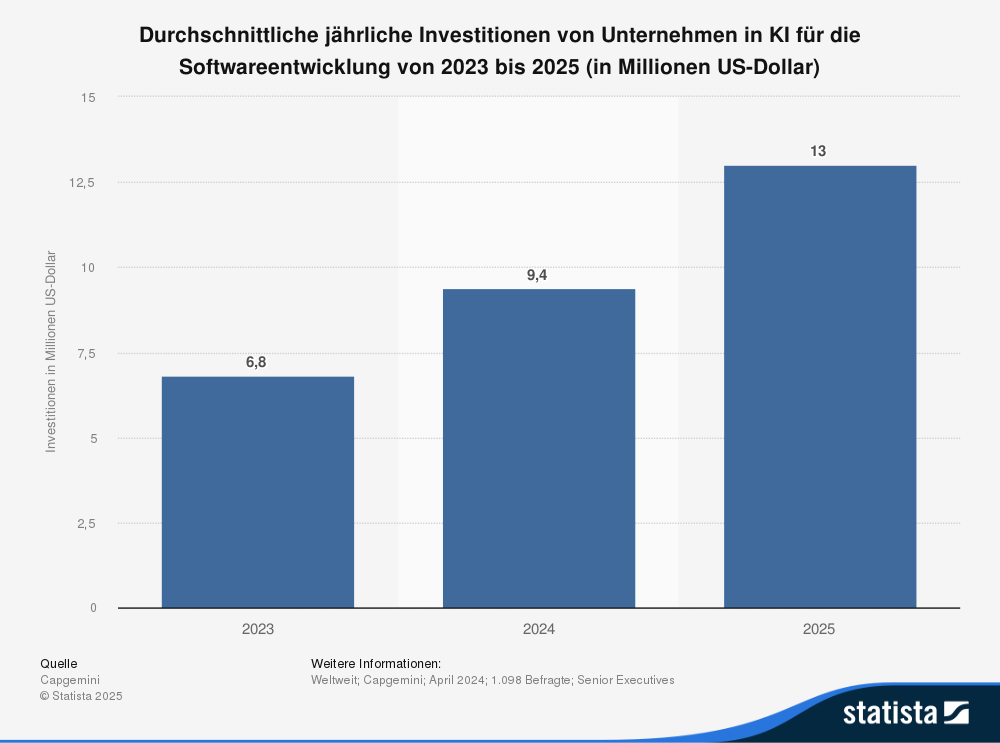
\includegraphics[width=0.7\textwidth]{images/abbildungen/statistic_id1481131_jaehrliche-investitionen-von-unternehmen-in-ki-fuer-softwareentwicklung-bis-2025.png}
    \caption{Jährliche Investitionen von Unternehmen in KI für Softwareentwicklung 2023–2025. Quelle: Capgemini~\cite{statista_ki_investitionen_2025}.}
    \label{fig:ki-investitionen}
\end{figure}

Allerdings werfen diese Entwicklungen auch kontroverse Fragen auf: In welchem
Maße verändert die zunehmende Abhängigkeit von KI-Tools die Rollen und
Kompetenzen von Softwareentwickler:innen? Wie kann sichergestellt werden, dass
durch KI-gestützte Automatisierung weiterhin qualitativ hochwertige, wartbare
und sichere Software entsteht~\cite{siebert_generative_2024}? Hinzu kommt, dass
die Softwareentwicklung durch agile Methoden wie Scrum oder Kanban bereits
stark dynamisiert ist. Die zusätzliche Integration von KI als Tool oder
„Co-Entwickler“ erhöht die Anforderungen an Prozessgestaltung, Rollenverteilung
und Qualitätsmanagement weiter.



\section{Zielsetzung und Fragestellungen}
Das Ziel dieser Arbeit ist es, die Auswirkungen von KI auf die Softwareentwicklung zu analysieren und praxisnahe Handlungsempfehlungen für Unternehmen und Entwickler abzuleiten. Dabei werden insbesondere folgende Forschungsfragen untersucht:

\begin{itemize}
    \item[FF-1] Wie verändert generative KI traditionelle Entwicklungspraktiken in der Softwareentwicklung?
    \item[FF-2] Welche spezifischen Herausforderungen entstehen durch KI-gestützte Softwareentwicklung hinsichtlich Sicherheit, Ethik und Code-Qualität?
    \item[FF-3] Wie kann Generative KI Softwareentwickler in einem agilen Entwicklungsprozess unterstützen? 
    \item[FF-4] Wie lassen sich bestehende generative KI-Tools (Cursor, GitHub Copilot, v0 etc.) in den Entwicklungsprozess einer React-Native-App integrieren, und welchen Einfluss hat das auf Entwicklungszeit und Code-Qualität?
    % \item[FF-4] Welche langfristigen Implikationen hat die Nutzung von KI auf die Rolle und Qualifikation von Softwareentwicklern?
    % \item[FF-5] Welche wirtschaftlichen und organisatorischen Auswirkungen hat die Integration von KI auf Softwareunternehmen und den Arbeitsmarkt?
\end{itemize}

Darüber hinaus wird ein praktisches Beispiel in Form einer React Native-App (Locals) angeführt, um zu untersuchen, wie bestehende generative KI-Tools (etwa Cursor, GitHub Copilot etc.) in einen realen Entwicklungsprozess integriert werden können.

\section{Methodik}

Die Arbeit folgt einem literaturbasierten, qualitativen Ansatz, um ein
umfassendes Bild der Potenziale und Herausforderungen generativer KI in der
Softwareentwicklung zu zeichnen. Ziel ist es, die aktuelle Forschungslage
systematisch zu erfassen, zu bewerten und praxisrelevante Schlüsse zu ziehen.
Die Methodik gliedert sich in folgende Schritte:

\begin{enumerate}
    % 1. punkt überprüfen: springer link & weiter quellen?
    \item \textbf{Literaturrecherche:} Umfassende Analyse wissenschaftlicher Publikationen aus IEEE Xplore, arXiv, SpringerLink sowie den in der Literaturdatenbank dieser Arbeit aufgeführten Fachquellen mit Fokus auf aktuelle Entwicklungen in der KI-gestützten Softwareentwicklung.
    \item \textbf{Kategorisierung der Forschungsthemen:} Strukturierte Erfassung und Gruppierung zentraler Themenfelder wie Automatisierung, Produktivität, Sicherheit und ethische Fragestellungen.
    \item \textbf{Vergleichende Analyse:} Systematischer Vergleich und Gegenüberstellung der Chancen und Herausforderungen auf Basis ausgewählter Studien und Fachbeiträge.
    \item \textbf{Synthese und Ableitung von Schlussfolgerungen:} Entwicklung praxisorientierter Empfehlungen für Unternehmen und Entwickler:innen zur Integration von KI in der Softwareentwicklung.
    \item \textbf{Praktische Demonstration:} Ergänzend zur Literaturauswertung wird ein Map-Screen (interaktive Kartenansicht) in der React Native-App „Locals“ exemplarisch implementiert. Dabei kommen verschiedene generative KI-Tools (u.a. Cursor, v0, GitHub Copilot) zum Einsatz, um die Unterstützung bei Code-Generierung, Testing und Qualitätsverbesserung zu evaluieren. Die gewonnenen Erkenntnisse aus diesem praktischen Teil werden systematisch mit den theoretischen Ergebnissen abgeglichen.
\end{enumerate}

Dieses methodische Vorgehen ermöglicht es, den aktuellen Forschungsstand
kritisch einzuordnen, praxisnahe Einblicke zu gewinnen und fundierte
Empfehlungen für die erfolgreiche Nutzung generativer KI in der
Softwareentwicklung abzuleiten.


% \section{Aufbau der Arbeit}
% Die Arbeit gliedert sich in folgende Kapitel:


\begin{itemize}
    \item \textbf{Kapitel 2:} Theoretische Grundlagen, in denen relevante Definitionen und Technologien der Künstlichen Intelligenz sowie Beispiele für generative KI-Tools vorgestellt werden.
    \item \textbf{Kapitel 3:} Chancen durch KI, mit einem Fokus auf Effizienzsteigerung und neuen Werkzeugen.
    \item \textbf{Kapitel 4:} Herausforderungen, einschließlich Sicherheits- und Datenschutzaspekten sowie ethischen Fragen.
    \item \textbf{Kapitel 5:} Fazit und Ausblick, mit einer Zusammenfassung der Ergebnisse und Handlungsempfehlungen.
\end{itemize}

\section{Abgrenzung}
Die Arbeit konzentriert sich auf die theoretische Analyse der Chancen und Herausforderungen von KI in der Softwareentwicklung. Folgende Aspekte werden bewusst ausgeklammert:

\begin{itemize}
    \item \textbf{Technische Implementierungen:} Es werden keine neuen KI-Modelle oder Algorithmen entwickelt.
    \item  \textbf{Empirische Studien:} Die Arbeit basiert auf einer literaturgestützten Analyse und führt keine Befragungen oder Experimente durch.
    \item \textbf{Rechtliche Rahmenbedingungen:} Eine detaillierte Untersuchung rechtlicher oder regulatorischer Aspekte wird nicht vorgenommen.
\end{itemize}

Obwohl ein begrenzter praktischer Teil in Form einer Funktionsimplementierung gezeigt wird, dient dieser in erster Linie als Proof of Concept. Eine umfassende empirische Evaluierung oder die Entwicklung eigener KI-Modelle findet nicht statt.

% Die Softwareentwicklung erlebt durch den Einsatz Künstlicher Intelligenz (KI) einen tiefgreifenden Wandel. Insbesondere generative KI-Modelle wie Large Language Models (LLMs) verändern etablierte Entwicklungspraktiken, indem sie Code generieren, automatisierte Tests durchführen und Entwicklungsprozesse effizienter gestalten. Diese Fortschritte werfen jedoch auch zentrale Fragen zur Sicherheit, zu ethischen Implikationen und zur langfristigen Rolle von Entwicklern auf.
%
% Erste Studien zeigen, dass KI-gestützte Tools signifikante Produktivitätssteigerungen ermöglichen, aber auch potenzielle Risiken wie Sicherheitslücken oder algorithmische Verzerrungen mit sich bringen. Daher ist es essenziell, eine fundierte wissenschaftliche Analyse durchzuführen, um Chancen und Herausforderungen umfassend zu bewerten.
%
% Diese Arbeit untersucht, wie KI-gestützte Softwareentwicklung die Produktivität und Qualität von Software beeinflusst, welche Herausforderungen sich daraus ergeben und welche praxisorientierten Anwendungen sich bereits abzeichnen. Dabei werden sowohl technologische als auch wirtschaftliche und gesellschaftliche Aspekte beleuchtet.

\chapter{Theoretische Grundlagen}
Leitfragen:

1. Was ist (generative) Künstliche Intelligenz (KI)?

2. Welche Unterscheidungen gibt es (z.B. schwache/starke KI, klassische/generative KI)?

3. Welche Basistechnologien, Modelle und Algorithmen sind relevant für die Softwareentwicklung?

\section{Künstliche Intelligenz: Definitionen und Technologien}
\input{content/Grundlagen/02_01_Künstliche_Intelligenz.tex}

\subsection{Beispiele für generative KI-Tools in der Praxis}
Generative KI-Tools sind heute in der Softwareentwicklung weit verbreitet und
decken ein breites Spektrum an Aufgaben ab -- von der Code-Vervollständigung
über automatische Testgenerierung bis hin zur Unterstützung ganzer
Entwicklungsprojekte. Im Folgenden werden vier prominente Tools vorgestellt,
die in der Praxis besonders relevant sind: \textbf{GitHub Copilot},
\textbf{TabNine}, \textbf{Cursor AI} und \textbf{Devin AI}.

\paragraph{GitHub Copilot}
GitHub Copilot ist ein KI-basierter Codeassistent, der Entwicklern direkt im
IDE-Kontext Vorschläge für Code-Snippets, ganze Funktionen und sogar Tests
macht. Die Integration erfolgt beispielsweise in Visual Studio Code, IntelliJ
oder Eclipse. Copilot basiert auf dem OpenAI Codex-Modell und kann mit
Kommentaren oder natürlicher Sprache gesteuert werden. Typische Einsatzfelder
sind das schnelle Prototyping, die Generierung von Boilerplate-Code, aber auch
die Hilfestellung für Einsteiger und Onboarding-Prozesse.

\begin{quote}
    \enquote{GitHub Copilot can assist in quick prototyping of code by generating foundational code structure based on natural language description of the feature. It can assist in boilerplate code generation by providing the class and interface definition generation, API and Database Schema creation. Both of these features combined improve the developer efficiency and enhanced code quality.}
    \cite[S.~8]{donvir_role_2024}
\end{quote}

Praxiserfahrung zeigt, dass GitHub Copilot die Entwicklung etwa einer
React-Anwendung deutlich beschleunigen kann, indem es Codevorschläge für
Authentifizierung, Routing und Formularvalidierung generiert und Fehlerbehebung
unterstützt. Entwickler betonen, dass der Review und die Überprüfung der
generierten Vorschläge dennoch unerlässlich bleiben \cite{kerr_github_nodate}.

\paragraph{TabNine}
TabNine ist ein weiteres KI-gestütztes Tool zur Code-Vervollständigung, das
ursprünglich auf GPT-2 basierte und heute ein eigenes Modell nutzt. Es kann
Codevorschläge in Echtzeit für verschiedene Sprachen machen und passt sich über
die Zeit an den Coding-Stil des jeweiligen Entwicklers an. TabNine unterstützt
alle gängigen IDEs und bietet eine Chat-Funktion, um gezielt Code-Fragen zu
stellen. Besonders geschätzt wird die Flexibilität durch lokale und
cloudbasierte Modelle sowie die Anpassung an unterschiedliche
Datenschutzanforderungen \cite[S.~9]{donvir_role_2024}.

\paragraph{Cursor AI}
Cursor AI repräsentiert die nächste Generation von KI-Entwicklungstools. Es ist
in der Lage, auf Basis natürlicher Sprache ganze Applikationen zu generieren,
nutzt Techniken wie Retrieval-Augmented Generation (RAG) und Agentic AI und
kann selbstständig Code verfeinern und Projekte strukturieren. Der Fokus liegt
auf End-to-End-Entwicklung und vollständiger Projektgenerierung, was
insbesondere für Prototyping oder den schnellen Aufbau komplexer
Softwarelösungen geeignet ist.

\begin{quote}
    \enquote{Cursor AI can generate the entire codebase of the application from the feature description of the project provided in natural language. It uses advanced AI concepts such as Retrieval Augmented Generation (RAG), Agentic AI, and prompt chaining to achieve its objectives and provides a high degree of automation in software development.}
    \cite[S.~10]{donvir_role_2024}
\end{quote}

\paragraph{Devin AI}
Devin AI geht noch einen Schritt weiter und bezeichnet sich selbst als
\enquote{AI Software Engineer}. Devin kann komplette Softwareprojekte auf Basis
von Anforderungen in natürlicher Sprache umsetzen, das Projekt in einzelne
Aufgaben herunterbrechen, automatisiert testen und sogar Deployment-Skripte
erstellen. Ein wesentliches Merkmal ist die Fähigkeit zur langfristigen Planung
und zur kontinuierlichen Anpassung an neue Anforderungen
\cite[S.~11]{donvir_role_2024}.

\vspace{1em}
\noindent
\textbf{Typische Einsatzszenarien}

Die beschriebenen Tools werden in der Praxis in unterschiedlichen Bereichen
eingesetzt:
\begin{itemize}
    \item \textbf{Code-Generierung und Vervollständigung:} Automatisiertes Schreiben von Code, Vorschläge für Funktionen, Klassen, API-Integration etc.
    \item \textbf{Test- und Debugging-Unterstützung:} Generierung von Unit- und Integrationstests, Identifikation von Fehlern und Vorschläge für Bugfixes.
    \item \textbf{Projekt-Scaffolding und Boilerplate:} Automatisches Erstellen von Grundstrukturen für neue Projekte.
    \item \textbf{End-to-End-Entwicklung:} Vollständige Umsetzung von Projektanforderungen inklusive Deployment-Skripten und CI/CD-Konfiguration \cite[S.~11]{donvir_role_2024}.
\end{itemize}

\vspace{1em}
\noindent
\textbf{Vorteile und Grenzen in der Praxis}

Die Integration generativer KI-Tools führt zu Zeitersparnis, konsistenterem
Code und einer schnelleren Einarbeitung neuer Entwickler. Gleichzeitig sind
Review-Prozesse und ein kritischer Umgang mit den generierten Vorschlägen
unerlässlich, um Qualitäts- und Sicherheitsrisiken zu minimieren.
Fortgeschrittene Tools wie Cursor AI oder Devin AI bieten ein hohes Maß an
Automatisierung, sind aber oft kostenintensiv und noch nicht für alle
Anwendungsfälle ausgereift \cite[S.~13]{donvir_role_2024}.

% \vspace{1em}
% \noindent
% \textbf{Quellen:}
% \begin{itemize}
%     \item Donvir, A. et al. (2024): \textit{The Role of Generative AI Tools in
%               Application Development: A Comprehensive Review of Current Technologies and
%               Practices} \cite{donvir_role_2024}
%     \item Kerr, K. (2025): \textit{GitHub for Beginners: Building a React App with GitHub
%               Copilot - The GitHub Blog} \cite{kerr_github_nodate}
% \end{itemize}


\subsection{Wichtige Algorithmen und Modelle in der Softwareentwicklung}
Die Integration generativer Künstlicher Intelligenz (KI) in der
Softwareentwicklung basiert maßgeblich auf fortschrittlichen Modellen und
Algorithmen. Im Zentrum stehen insbesondere Large Language Models (LLMs) und
Transformer-Architekturen, die als Grundlage moderner Coding-Tools wie GitHub
Copilot, Cursor oder v0 dienen. Im Folgenden werden die wichtigsten Modelle,
deren Funktionsweise und deren Bedeutung für typische
Softwareentwicklungsaufgaben erläutert.

\paragraph{Grundprinzipien und Funktionsweise moderner KI-Modelle}

Large Language Models (LLMs), wie beispielsweise GPT-4 oder Code Llama, sind
tiefenlernende neuronale Netze, die auf sehr großen Mengen von Quellcode und
natürlicher Sprache trainiert wurden. Sie nutzen Transformer-Architekturen, die
durch sogenannte Self-Attention-Mechanismen Kontextinformationen über lange
Sequenzen hinweg erfassen können. Dies ermöglicht es ihnen, sowohl syntaktisch
als auch semantisch komplexe Strukturen – wie etwa Code-Logik oder Designmuster
– zu erkennen und zu generieren~\cite{nguyen-duc_generative_2023,
    esposito_generative_2025}.

Diffusionsmodelle spielen hingegen vor allem in der Bild- und Grafikgenerierung
eine Rolle und sind für den textbasierten Softwareentwicklungsprozess bislang
von untergeordneter Bedeutung. Für Aufgaben wie Codegenerierung und
Architektur-Design sind LLMs und Transformer-Modelle
maßgeblich~\cite{weisz_design_2024}.

\paragraph{Beispiele für KI-Modelle in Coding-Tools}

Moderne Coding-Assistenzsysteme wie \textit{GitHub Copilot}, \textit{Cursor}
und \textit{v0} basieren auf Varianten großer Sprachmodelle, meist speziell auf
Programmcode vortrainiert (z.\,B. OpenAI Codex, Code Llama, StarCoder). Diese
Modelle können anhand des jeweiligen Kontexts (z.\,B. bestehender Code,
Kommentare, Projekthistorie) automatisiert neue Code-Abschnitte generieren,
Vorschläge zur Fehlerbehebung machen oder Testfälle
entwerfen~\cite{coutinho_role_2024, esposito_generative_2025}.

Typische Anwendungsbereiche sind:
\begin{itemize}
    \item \textbf{Code-Generierung}: Erstellung neuer Funktionen, Methoden oder ganzer Module auf Basis von Kurzbeschreibungen oder natürlicher Sprache.
    \item \textbf{Testing und Qualitätssicherung}: Automatisierte Generierung von Unit-Tests und Testdaten, Unterstützung beim Review durch Erkennung von Anomalien oder Schwachstellen.
    \item \textbf{Architekturvorschläge}: Unterstützung bei der Auswahl geeigneter Softwarearchitekturen oder Design Patterns, teilweise mit Bezug auf bestehende Anforderungen oder Projektdaten~\cite{esposito_generative_2025}.
\end{itemize}

\paragraph{Rolle dieser Modelle für spezifische Aufgaben}

\begin{itemize}
    \item \textbf{Codegenerierung:} LLMs können auf Grundlage von Prompts oder bestehenden Code-Fragmente eigenständig funktionsfähigen Quellcode erzeugen. Dies umfasst Routineaufgaben (z.\,B. Boilerplate-Code) ebenso wie komplexere Algorithmen.
    \item \textbf{Testing:} Modelle wie GPT-4 sind in der Lage, automatisiert Tests zu erzeugen, Testdaten zu variieren und gängige Fehlerbilder zu erkennen.
    \item \textbf{Architekturvorschläge:} Moderne LLMs unterstützen zunehmend beim Entwurf und bei der Dokumentation von Softwarearchitekturen, indem sie z.\,B. Requirements in Design-Vorschläge oder Diagramme übersetzen~\cite{esposito_generative_2025, nguyen-duc_generative_2023}.
\end{itemize}

\paragraph{Herausforderungen und Grenzen}

Trotz des enormen Potenzials bestehen aktuelle Herausforderungen:
\begin{itemize}
    \item \textbf{Halluzinationen und Fehleranfälligkeit}: Generative Modelle können syntaktisch korrekten, aber fachlich unpassenden oder sogar gefährlichen Code erzeugen.
    \item \textbf{Erklärbarkeit und Transparenz}: Die Nachvollziehbarkeit, wie ein Modell zu bestimmten Ergebnissen kommt, ist oft eingeschränkt~\cite{esposito_generative_2025, nguyen-duc_generative_2023}.
    \item \textbf{Domänenspezifisches Wissen}: Ohne Anpassung (Fine-Tuning) auf projektspezifische Daten sind die Modelle oft auf allgemeines Wissen beschränkt und berücksichtigen spezifische Anforderungen nur begrenzt.
\end{itemize}

\paragraph{Bezug zu den im Praxisteil genutzten Tools}

Die im Praxisteil eingesetzten Tools (\textit{GitHub Copilot, Cursor, v0})
nutzen genau diese Algorithmen, um Entwickler:innen bei alltäglichen
Entwicklungsaufgaben zu unterstützen. Sie liefern damit nicht nur klassische
Code-Vervollständigungen, sondern wirken zunehmend als kollaborative Partner im
gesamten Entwicklungsprozess – von Architektur über Implementierung bis zum
Test~\cite{esposito_generative_2025, nguyen-duc_generative_2023}.



\section{Generative KI-Tools: Funktion und Anwendung}
\label{sec:generative-ki-tools}

Generative KI-Tools wie GitHub Copilot, Cursor oder v0 prägen den modernen
Softwareentwicklungsprozess entscheidend. Ihre Hauptfunktion besteht darin,
natürliche Sprache (Prompts) in ausführbaren Code, Testfälle oder
Dokumentationen umzusetzen. Damit verändern sie nicht nur technische Workflows,
sondern auch die Zusammenarbeit in Entwicklungsteams und die Anforderungen an
Kompetenzen der Beteiligten \cite{weisz_design_2024}.

\subsubsection{Grundfunktion generativer KI-Tools}

Die zugrundeliegenden Large Language Models (LLMs) ermöglichen das sogenannte
Prompt-basiertes Entwicklungsparadigma: Entwickler:innen beschreiben eine
Aufgabe in natürlicher Sprache – das Tool generiert dazu passende Vorschläge.
Diese erscheinen als Code Completion direkt beim Tippen oder als komplette
Funktionsblöcke \cite{kerr_github_nodate, weisz_design_2024}. Neuere Ansätze
wie SENAI integrieren generative KI von Anfang an in den
Software-Engineering-Prozess und erlauben eine hochautomatisierte,
KI-zentrierte Entwicklung \cite{saad_senai_2025}.

Systematische Literaturübersichten zeigen, dass die Integration generativer KI
in Entwicklungsumgebungen das Nutzererlebnis, die Akzeptanz und den praktischen
Nutzen maßgeblich beeinflusst. Insbesondere Aspekte wie Transparenz, Usability
und Feedbackmechanismen entscheiden über den Erfolg im Alltag
\cite{sergeyuk_human-ai_2025}.

\subsubsection{Schnittstellen und Integration in Entwicklungsumgebungen}

Die praktische Nutzung generativer KI erfolgt meist über Plugins (z. B. für
Visual Studio Code oder JetBrains IDEs) oder via API. Typischerweise
interagieren Entwickler:innen mit dem KI-Tool im Kontext der gewohnten
Umgebung, wodurch Aufgaben wie Refactoring, Testing oder Dokumentation direkt
integriert werden können \cite{kerr_github_nodate, shi_ai-assisted_2023,
    weisz_design_2024}.

Besonderes Augenmerk liegt inzwischen auch auf Barrierefreiheit: KI-gestützte
Assistenzsysteme eröffnen etwa Entwickelnden mit Sehbeeinträchtigung neue
Teilhabemöglichkeiten, vorausgesetzt die Tools sind entsprechend gestaltet
\cite{flores-saviaga_impact_2025}.

\subsubsection{Beispielhafte Workflows: Pair Programming mit Copilot}

Beim Pair Programming mit Copilot werden Aufgaben in Form von Prompts gestellt,
Copilot generiert daraufhin Codevorschläge, die geprüft, angepasst oder
verworfen werden können. So unterstützt Copilot u. a. die Testautomatisierung,
das Refactoring und die Dokumentation in allen Phasen des
Entwicklungsprozesses. Studien belegen signifikante Beschleunigungseffekte bei
Routineaufgaben \cite{kerr_github_nodate, weisz_design_2024,
    shi_ai-assisted_2023}. In agilen Teams kann generative KI zudem zur
Qualitätsbewertung und Dokumentation von Anforderungen beitragen
\cite{geyer_case_2025}.

\subsubsection{Vorteile und Optimierungspotenziale}

Der Einsatz generativer KI bietet zahlreiche Vorteile:
\begin{itemize}
    \item \textbf{Zeitersparnis:} Automatisierung von Routineaufgaben, Verkürzung von Entwicklungszyklen.
    \item \textbf{Verbesserte Codequalität:} Erkennung häufiger Fehler, Empfehlungen für Best Practices.
    \item \textbf{Niedrigere Einstiegshürden:} Unterstützung auch für weniger erfahrene Entwickler:innen durch kontextbasierte Vorschläge.
\end{itemize}
KI-gestützte Code Reviews fördern die Kollaboration zwischen Mensch und Maschine und erhöhen die Transparenz im Entwicklungsprozess \cite{alami_human_2025}. Kontinuierliche Modellverbesserung und flexible Integration in unterschiedliche Projekte steigern das Optimierungspotenzial weiter \cite{kerr_github_nodate, weisz_design_2024}.

\subsubsection{Grenzen und typische Fehlerquellen}

Zu den zentralen Herausforderungen zählen:
\begin{itemize}
    \item \textbf{Halluzinationen:} Syntaktisch korrekter, aber inhaltlich fehlerhafter oder unsicherer Code, vor allem bei vagen Prompts \cite{shi_ai-assisted_2023}.
    \item \textbf{Bias und Kontextdefizite:} Übernahme von Vorurteilen oder Nichtbeachtung spezifischer Projektregeln.
    \item \textbf{Sicherheitsrisiken:} Vorschläge für unsicheren Code (z. B. Hardcoded Credentials), die explizit überprüft werden müssen \cite{shi_ai-assisted_2023}.
    \item \textbf{Übermäßiges Vertrauen:} Unkritische Übernahme von KI-Vorschlägen ohne Review durch erfahrene Entwickler:innen \cite{weisz_design_2024}.
\end{itemize}

\subsubsection{Designprinzipien für den produktiven und sicheren Einsatz}

Für die sichere Nutzung generativer KI-Tools werden in der Literatur folgende
Designprinzipien empfohlen \cite{weisz_design_2024}:
\begin{itemize}
    \item \textbf{Design for Mental Models:} Nutzer:innen sollen die Funktionsweise und Grenzen nachvollziehen können.
    \item \textbf{Design for Appropriate Trust \& Reliance:} Feedbackmechanismen müssen sowohl Vertrauen fördern als auch zur kritischen Prüfung anregen.
    \item \textbf{Design for Imperfection:} Aktive Hinweise auf mögliche Fehler und die Befähigung zur Korrektur sind essenziell.
\end{itemize}

Die Gestaltung generativer GUIs und Entwicklungsprozesse muss diese Prinzipien
berücksichtigen, um eine nachhaltige und verantwortungsvolle Integration zu
ermöglichen \cite{lee_towards_2025, chen_genui_2025, gill_agile_2025}.
Flexibilität, Feedback und kontinuierliche Anpassung sind Schlüssel zum Erfolg.

% Optional: Kurzbezug auf Kapitel 3 (Praxisbeispiel), falls erwünscht
% Wie in Kapitel 3 praktisch demonstriert, lassen sich diese Prinzipien in der Entwicklung von React Native-Anwendungen mit KI-Tools exemplarisch umsetzen.




\chapter{Praktische Demonstration}
Die bisherigen Kapitel haben die grundlegenden Technologien, Chancen und
Herausforderungen generativer KI in der Softwareentwicklung theoretisch
beleuchtet. Im folgenden Kapitel wird dieses Wissen nun praktisch angewendet.
Anhand der exemplarischen Implementierung einer interaktiven Kartenansicht
(„Map-Screen“) in der React Native-App \textit{Locals} wird demonstriert, wie
verschiedene generative KI-Tools (z.\,B. GitHub Copilot, Cursor, Bolt) den
Entwicklungsprozess konkret unterstützen können. Ziel ist es, die praktische
Integration, Arbeitsweise sowie Vor- und Nachteile der Tools unter
realistischen Bedingungen zu untersuchen.
\section{Zielsetzung und Vorgehen}
\label{sec:zielsetzung-vorgehen}

Am Beispiel der exemplarischen Implementierung einer interaktiven Kartenansicht
(„Map-Screen“) in der mobilen App „Locals“ wird untersucht, wie moderne
KI-gestützte Tools den Entwicklungsprozess unterstützen, in welchen Bereichen
sie ihre Stärken ausspielen können und wo ihre Grenzen sichtbar werden.
Aufbauend auf den zuvor beschriebenen theoretischen Grundlagen bietet dieses
Praxisbeispiel die Gelegenheit, zentrale Konzepte und Annahmen empirisch zu
überprüfen und kritisch zu reflektieren.

Die Entscheidung, den Fokus auf die Entwicklung einer interaktiven
Kartenansicht zu legen, ist aus mehreren Gründen besonders sinnvoll. Erstens
handelt es sich bei Map-Views um zentrale und technisch anspruchsvolle Features
in Event- und Social-Apps, da sie die Integration verschiedener Technologien
wie Geolocation, Datenmanagement, UI/UX-Design und Filterfunktionen erfordern.
Zweitens vereint diese Aufgabe klassische Frontend-Herausforderungen,
beispielsweise im Bereich State-Management und UI-Logik, mit der Integration
externer Libraries wie \texttt{react-native-maps} oder der Google Maps API.
Gerade durch diese Vielschichtigkeit eignet sich die Map-View besonders gut, um
die Leistungsfähigkeit generativer KI-Tools im realen Entwicklungsprozess
kritisch zu beleuchten. Nicht zuletzt unterstreicht auch der unmittelbare
Nutzen für die Anwender:innen die hohe Praxisrelevanz des gewählten Beispiels.

Für die Umsetzung wurden drei führende KI-basierte Entwicklungstools
ausgewählt, die aktuelle Trends und Methoden im Bereich der KI-gestützten
Softwareentwicklung abbilden. Zum einen kommt \textit{GitHub Copilot} zum
Einsatz, ein kontextsensitiver Code-Assistent mit Echtzeit-Vervollständigung,
der automatische Vorschläge für Funktionen, Tests und Dokumentation generiert
und sich direkt in gängige IDEs integriert~\cite{github_copilot_2025}.
Ergänzend wird \textit{Cursor} verwendet, ein KI-basierter Editor, der durch
Multi-Line-Edits, Prompt Chaining, Fehlerdiagnose und eine dialogorientierte
Benutzeroberfläche die Umsetzung komplexer Aufgaben unterstützt und
plattformübergreifend einsetzbar ist~\cite{cursor_welcome_2025}. Als drittes
Tool kommt \textit{Bolt} hinzu, eine cloudbasierte Entwicklungsumgebung, die
ohne lokale Installation auskommt und die Entwicklung sowie das Deployment
direkt aus Prompts heraus ermöglicht. Bolt unterstützt mehrere Plattformen,
bietet Live-Bearbeitung und Teamfunktionen~\cite{bolt_support_2025}.

Die vergleichende Analyse dieser drei Tools ermöglicht es, unterschiedliche
Formen der Interaktion zwischen Mensch und KI im realen Entwicklungsalltag zu
bewerten, von klassischen Code-Vervollständigern wie Copilot über
dialogorientierte Systeme wie Cursor bis hin zu agentenbasierten
Komplettumgebungen wie Bolt. Dadurch lassen sich Stärken, Schwächen und
bestmögliche Einsatzszenarien generativer KI-Tools in der Praxis gezielt
herausarbeiten.


\section{Vorstellung der App \glqq Locals\grqq}
\subsection{Architektur und Aufbau}

Die App \textit{Locals} ist eine mobile Anwendung, die Nutzer:innen dabei
unterstützt, lokale Events zu entdecken, zu erstellen und zu verwalten. Sie
richtet sich insbesondere an ein junges, urbanes Publikum und fördert soziale
Interaktionen im Kontext gemeinsamer Veranstaltungen.

% \begin{figure}[htbp]
%     \centering
%     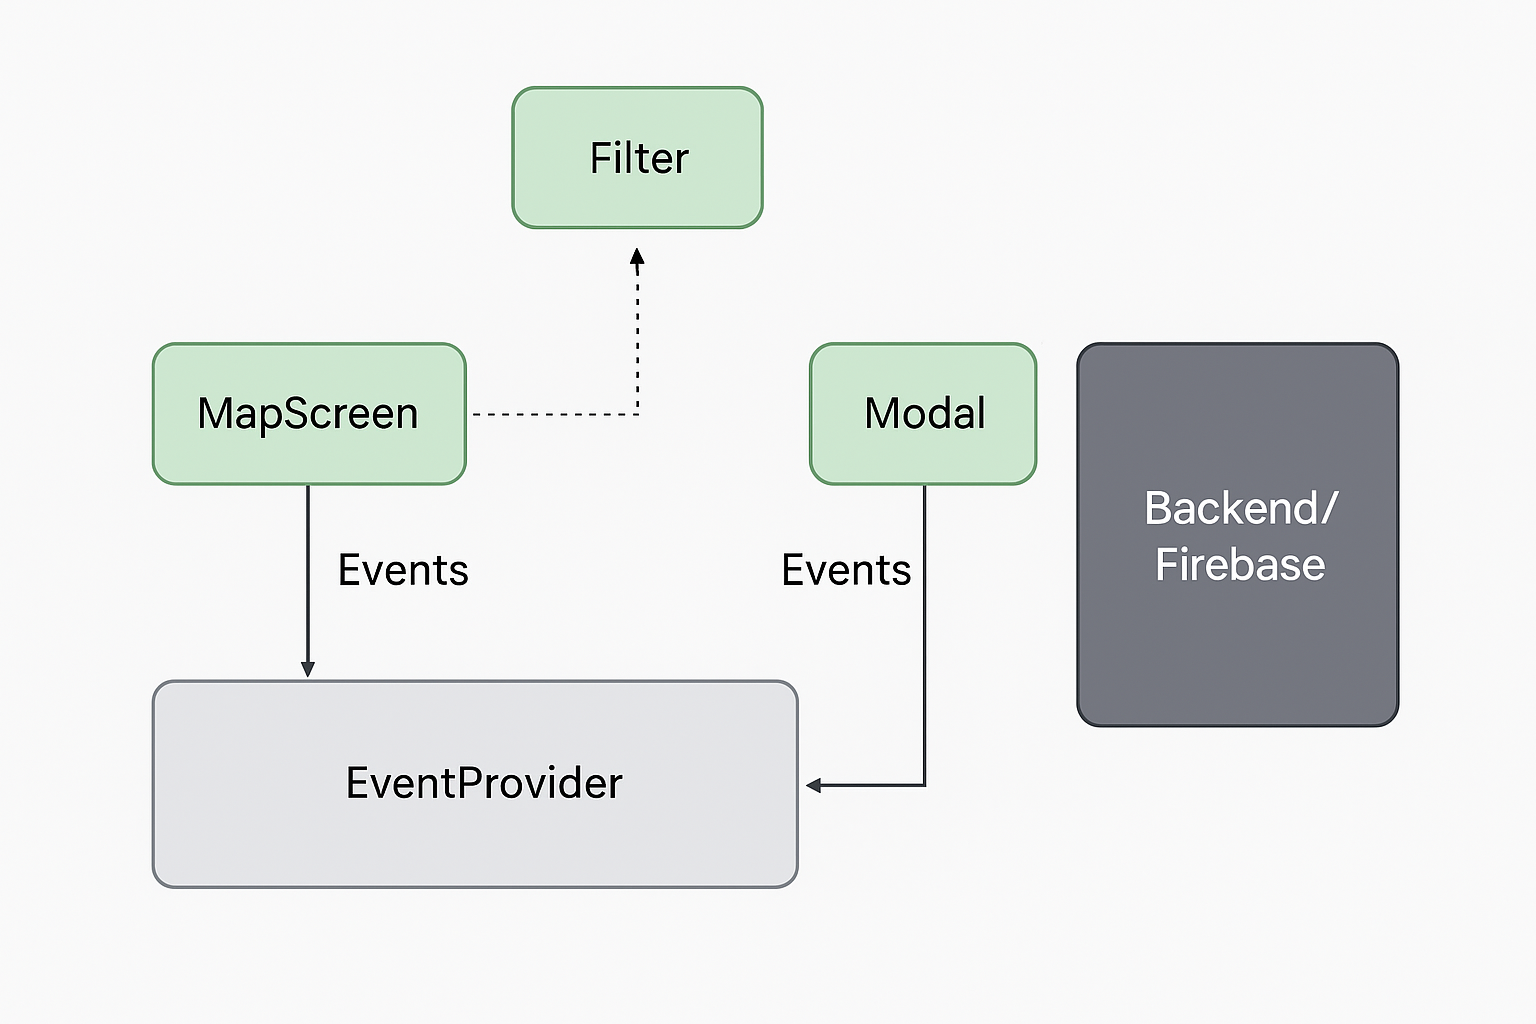
\includegraphics[width=0.95\textwidth]{images/architekturdiagramm_locals.png}
%     \caption{Architektur der App „Locals“: Darstellung der Hauptkomponenten (MapScreen, Filter, Modal, EventProvider, Backend/Firebase) und deren Datenflüsse.}
%     \label{fig:architektur-locals}
% \end{figure}

\subsubsection{Technologischer Stack und Architektur}

Der technologische Stack von \textit{Locals} wurde gezielt so ausgewählt, dass
eine moderne, plattformübergreifende Entwicklung und eine reibungslose User
Experience möglich sind:
\begin{itemize}
    \item \textbf{Frontend:} Entwicklung mit React Native, TypeScript und Expo für eine performante Bereitstellung auf iOS und Android.
    \item \textbf{Backend:} Verwendung von Firebase zur Authentifizierung, Datenhaltung und Synchronisation.
    \item \textbf{Navigation:} Einsatz von \texttt{@react-navigation/native} und \texttt{expo-router} für ein modernes, tab-basiertes Navigationskonzept.
    \item \textbf{State-Management:} Implementierung eigener Context-Provider (\texttt{AuthProvider}, \texttt{EventsProvider}) für Authentifizierungs- und Eventdaten.
    \item \textbf{UI-Komponenten:} Nutzung von \texttt{@expo/vector-icons} und \texttt{lucide-react-native} für ein ansprechendes und konsistentes User Interface.
    \item \textbf{Maps \& Location:} Integration von \texttt{react-native-maps} und \texttt{expo-location} für eine interaktive Kartenansicht, die sowohl den Nutzerstandort als auch Events auf einer Karte visualisiert.
\end{itemize}

Die App ist modular aufgebaut und besteht aus drei zentralen Bereichen:
\begin{itemize}
    \item \textbf{Explore-Screen:} Zeigt einen Event-Feed, der sich nach Interessen und aktuellem Standort richtet.
    \item \textbf{Map-Screen:} Bietet eine interaktive Kartenansicht mit Event-Markern und Filterfunktion.
    \item \textbf{Profil-Screen:} Ermöglicht die Übersicht und Verwaltung eigener Events und Profildaten.
\end{itemize}

Während Explore- und Profil-Screen bereits Grundfunktionen aufweisen, wird der
Map-Screen im Rahmen dieser Arbeit als prototypisches Demonstrationsbeispiel
gezielt entwickelt und evaluiert. Die praktische Realisierung dieses Features
erfolgt unter Einsatz generativer KI-Tools und steht im Mittelpunkt der
folgenden Kapitel.

\subsubsection{Struktur der Haupteinstiegskomponente (\texttt{RootLayout})}

Die zentrale Einstiegskomponente der App ist das \texttt{RootLayout}. Diese
übernimmt das Laden benutzerdefinierter Fonts, die Einbindung von
Authentifizierungs- und Events-Kontexten sowie eine durchgängige Nutzerführung
nach dem Login. Die Navigation wird dabei strikt vom Authentifizierungsstatus
gesteuert, sodass nicht eingeloggte Nutzer:innen automatisch zur Login-Ansicht
weitergeleitet werden. Für die technische Umsetzung werden Hooks wie
\texttt{useAuth}, \texttt{useSegments} und \texttt{useRouter} eingesetzt.

\subsection{Bestehende Funktionalitäten}

Bereits implementierte Kernfunktionen von \textit{Locals} sind:
\begin{itemize}
    \item \textbf{Benutzerauthentifizierung:} Sichere Registrierung und Anmeldung über Firebase Authentication.
    \item \textbf{Profilverwaltung:} Verwaltung persönlicher Daten sowie Übersicht über besuchte und selbst erstellte Events.
    \item \textbf{Eventverwaltung:} Anlegen, Bearbeiten und Löschen von Events.
    \item \textbf{Tab-Navigation:} Ermöglicht den nahtlosen Wechsel zwischen den drei Hauptbereichen „Explore“, „Map“ und „Profil“.
    \item \textbf{Responsives Design:} Konsistente Darstellung auf verschiedenen Endgeräten durch Nutzung von \texttt{react-native-safe-area-context} und Expo UI-Komponenten.
\end{itemize}

Der Map-Screen ist als zentrales, innovatives Feature der App konzipiert. Die
Implementierung und Weiterentwicklung dieses Moduls wird im weiteren Verlauf
dieser Arbeit als praktisches Beispiel für den Einsatz generativer KI in der
Softwareentwicklung detailliert analysiert.


\section{Implementierung der interaktiven Kartenansicht mit KI-Unterstützung}
% TODO: stichpunkte als fließtext soweit möglich (reflexion & fazit). vielleicht auch in anderen abschnitten (kapitel 2, ab seite 10).

\subsection{Prompt-Setup: Einheitliche Aufgabenstellung für alle Tools}
\label{sec:prompt-setup}

Um eine objektive und vergleichbare Bewertung zu ermöglichen, wurde für die
Implementierung des Map-Screens in allen drei Tools (\textit{GitHub Copilot},
\textit{Cursor}, \textit{Bolt.new}) derselbe, detaillierte Prompt verwendet,
der die funktionalen und technischen Anforderungen klar definierte:

\begin{lstlisting}[]
    Create a Map Screen with Event Markers and Filter in React Native
    
    Create a React Native component called `MapScreen` that displays event markers on a map using event data from the `EventsProvider` context.
    
    ## Requirements
    
    ### Functionality
    - Use the list of events from the `EventsProvider` context.  
      (Access: `const { events, loading, error, refreshEvents } = useEvents();`)
    - Each event contains:
      - `docId: string`
      - `title: string`
      - `category: string`
      - `date: string`
      - `geoPoint: { latitude: number; longitude: number }`
    - Example Context Usage: const { events, loading, error, refreshEvents } = useEvents();
    - Display all events as markers on a map (`react-native-maps` or Expo MapView).
    - When a marker is tapped, show a callout or modal with event details (`title`, `time`, `category`, optional image/avatar).
    - Add filter options above the map (e.g. by category, date, distance).  
      Only display events that match active filters.
    - Handle loading and error states appropriately.
    
    ### UI/UX
    - Modern mobile UI with a clean filter bar on top, responsive marker popups, and a loading spinner.
    - Use functional components and React hooks (TypeScript).
    - Styling should be clean and minimal (simple css with StyleSheet prefered).
    - Map should fit all visible markers and allow user zoom/pan.
    - Compatible with Expo.
    
    ### File Structure
    - Main screen in `map.tsx`.
    - Optional: Reusable `EventMarker` component.
    
    ### Additional
    - Keep code modular, clean, and well-commented.
    - Focus on maintainability and clarity.
    - Use the attached layout (filter bar on top, map below, details as bottom sheet/callout) as a visual reference.
    
    ### Example Event Type (TypeScript)
    interface Event {
      docId: string;
      title: string;
      category: string;
      date: string;
      geoPoint: { latitude: number; longitude: number };
      // ...more fields possible
    }

    ## Goal
    A fully functional, modern React Native map screen with event markers, filter bar, marker popups, and proper handling of loading/error states -- ready to integrate into an Expo app.

    
    \end{lstlisting}

\noindent
\textbf{Hinweis:} Diese Aufgabenstellung wurde in allen Demonstrationen identisch genutzt, um die Unterschiede in Lösungsstrategie und Codequalität der Tools direkt vergleichbar zu machen.

\subsection{Demonstration mit GitHub Copilot}

\subsubsection{Setup und Vorgehen}
Die Entwicklung des Map-Screens wurde exemplarisch mit \textbf{GitHub Copilot}
in Visual Studio Code durchgeführt. Für größtmögliche Vergleichbarkeit kamen
ausschließlich die Copilot-Funktionen zum Einsatz, keine weiteren KI-Plugins.

\begin{figure}[htbp]
      \centering
      \vspace{1em}
      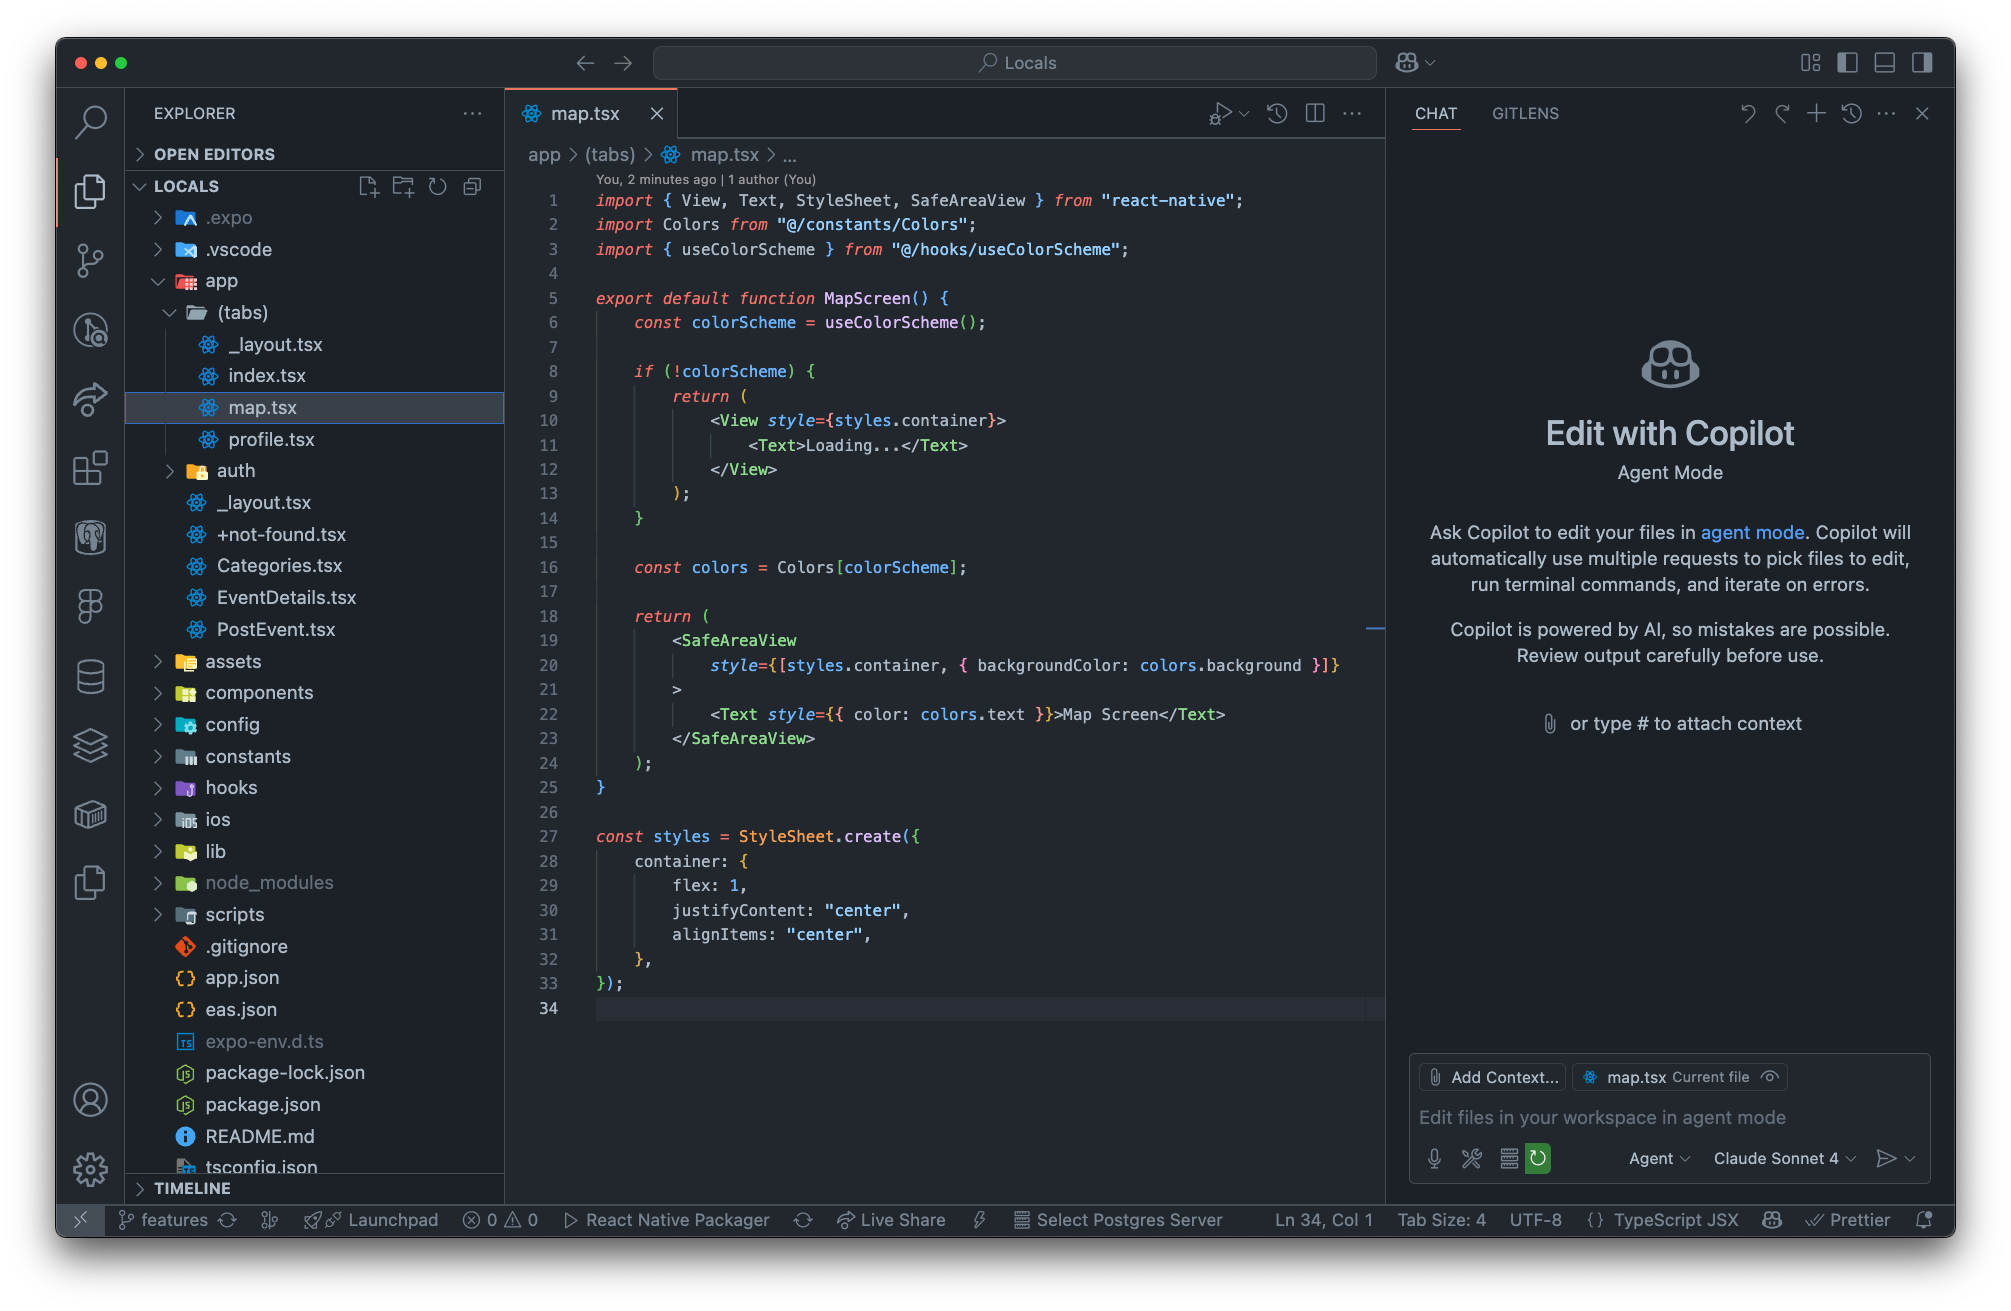
\includegraphics[width=1\textwidth]{images/copilot_screenshots/Screenshots Ist-Zustand-copilot.png}
      \caption{Ausgangszustand der Anwendung vor dem Einsatz von Copilot. \textit{Copilot-Demo}}
      \label{fig:copilot-istzustand}
\end{figure}

% TODO: muss ich alles aufzählen nicht nur z.b.?
Zu Beginn wurde die Entwicklungsumgebung vorbereitet (z.~B.\ Installation von
\texttt{react-native-maps} und \texttt{expo-location}). Die Aufgabenstellung
wurde als Kommentar oder Docstring auf Englisch eingefügt (\emph{siehe
      Abschnitt~\ref{sec:prompt-setup}}).

\subsubsection{Schrittweise Umsetzung und Reflexion}
Die Entwicklung erfolgte nach folgendem Muster:
\begin{enumerate}
      \item \textbf{Prompt definieren:} Pro Feature (z.\,B. Marker, Filter, Event-Details) wurde ein spezifischer Kommentar als Arbeitsanweisung eingefügt.
      \item \textbf{Vorschläge von Copilot akzeptieren oder anpassen:} Vorschläge wurden übernommen, angepasst oder verworfen.
      \item \textbf{Test und Dokumentation:} Nach jeder Änderung wurde der Code getestet und die Funktionsweise reflektiert.
      \item \textbf{Fehlersuche und Nacharbeit:} Fehlerhafte Vorschläge oder Bugs wurden durch Rücksprache mit Copilot, Recherche oder manuelle Nacharbeit behoben.
\end{enumerate}

\begin{figure}[htbp]
      \centering
      \vspace{1em}
      \begin{minipage}{0.48\textwidth}
            \centering
            \includegraphics[width=0.98\textwidth]{images/copilot_screenshots/implementation-rückmeldung-copilot-1.png}
      \end{minipage}
      \hfill
      \begin{minipage}{0.48\textwidth}
            \centering
            \includegraphics[width=0.98\textwidth]{images/copilot_screenshots/implementation-rückmeldung-copilot-2.png}
      \end{minipage}
      \caption{Rückmeldung und Hinweise von Copilot während der Implementierung. \textit{Copilot-Demo}}
      \label{fig:copilot-impl-pair}
\end{figure}

\noindent Die technische Umsetzung umfasste:
\begin{itemize}
      \item Anzeige aller Events als Marker (mit Kategorie und Titel) auf der Karte.
      \item Filterleiste zur Auswahl nach Kategorie und Datum.
      \item Darstellung von Event-Details beim Tippen auf einen Marker.
      \item Responsives Layout, modernes UI-Design, Fehler- und Ladezustände.
\end{itemize}

\begin{figure}[htbp]
      \centering
      \vspace{1em}
      \begin{minipage}{0.48\textwidth}
            \centering
            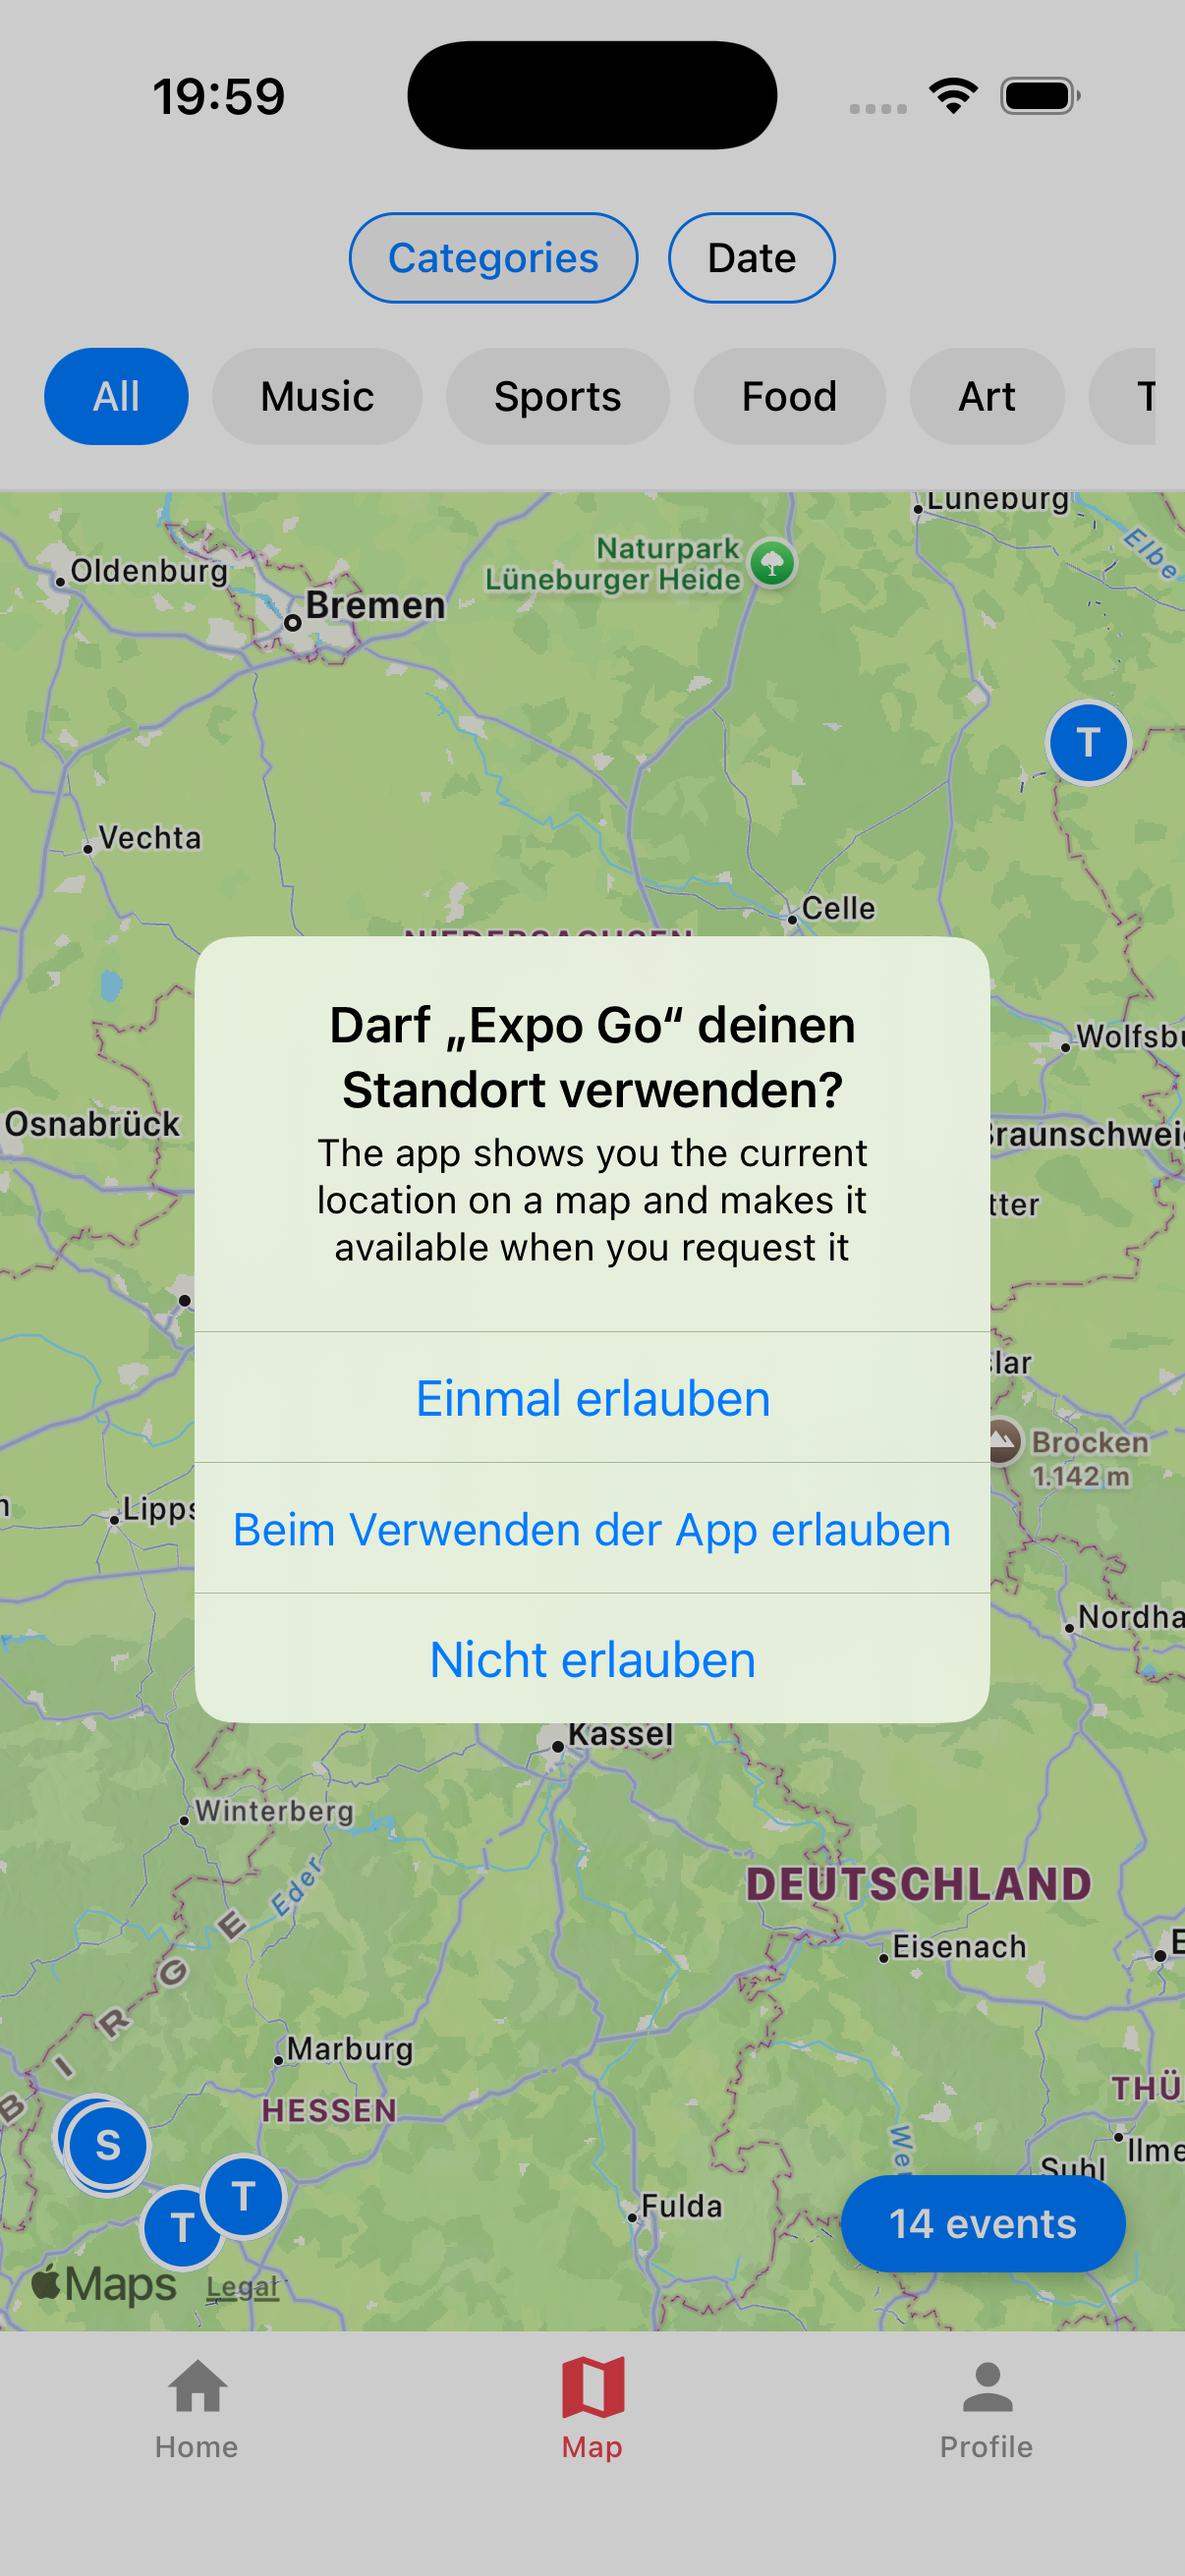
\includegraphics[width=\textwidth]{images/copilot_screenshots/6. 1. Version das MapScreens - Screenshot-copilot.png}
            \caption{Erste lauffähige Version des MapScreens nach KI-gestützter Entwicklung. \textit{Copilot-Demo}}
      \end{minipage}
      \hfill
      \begin{minipage}{0.48\textwidth}
            \centering
            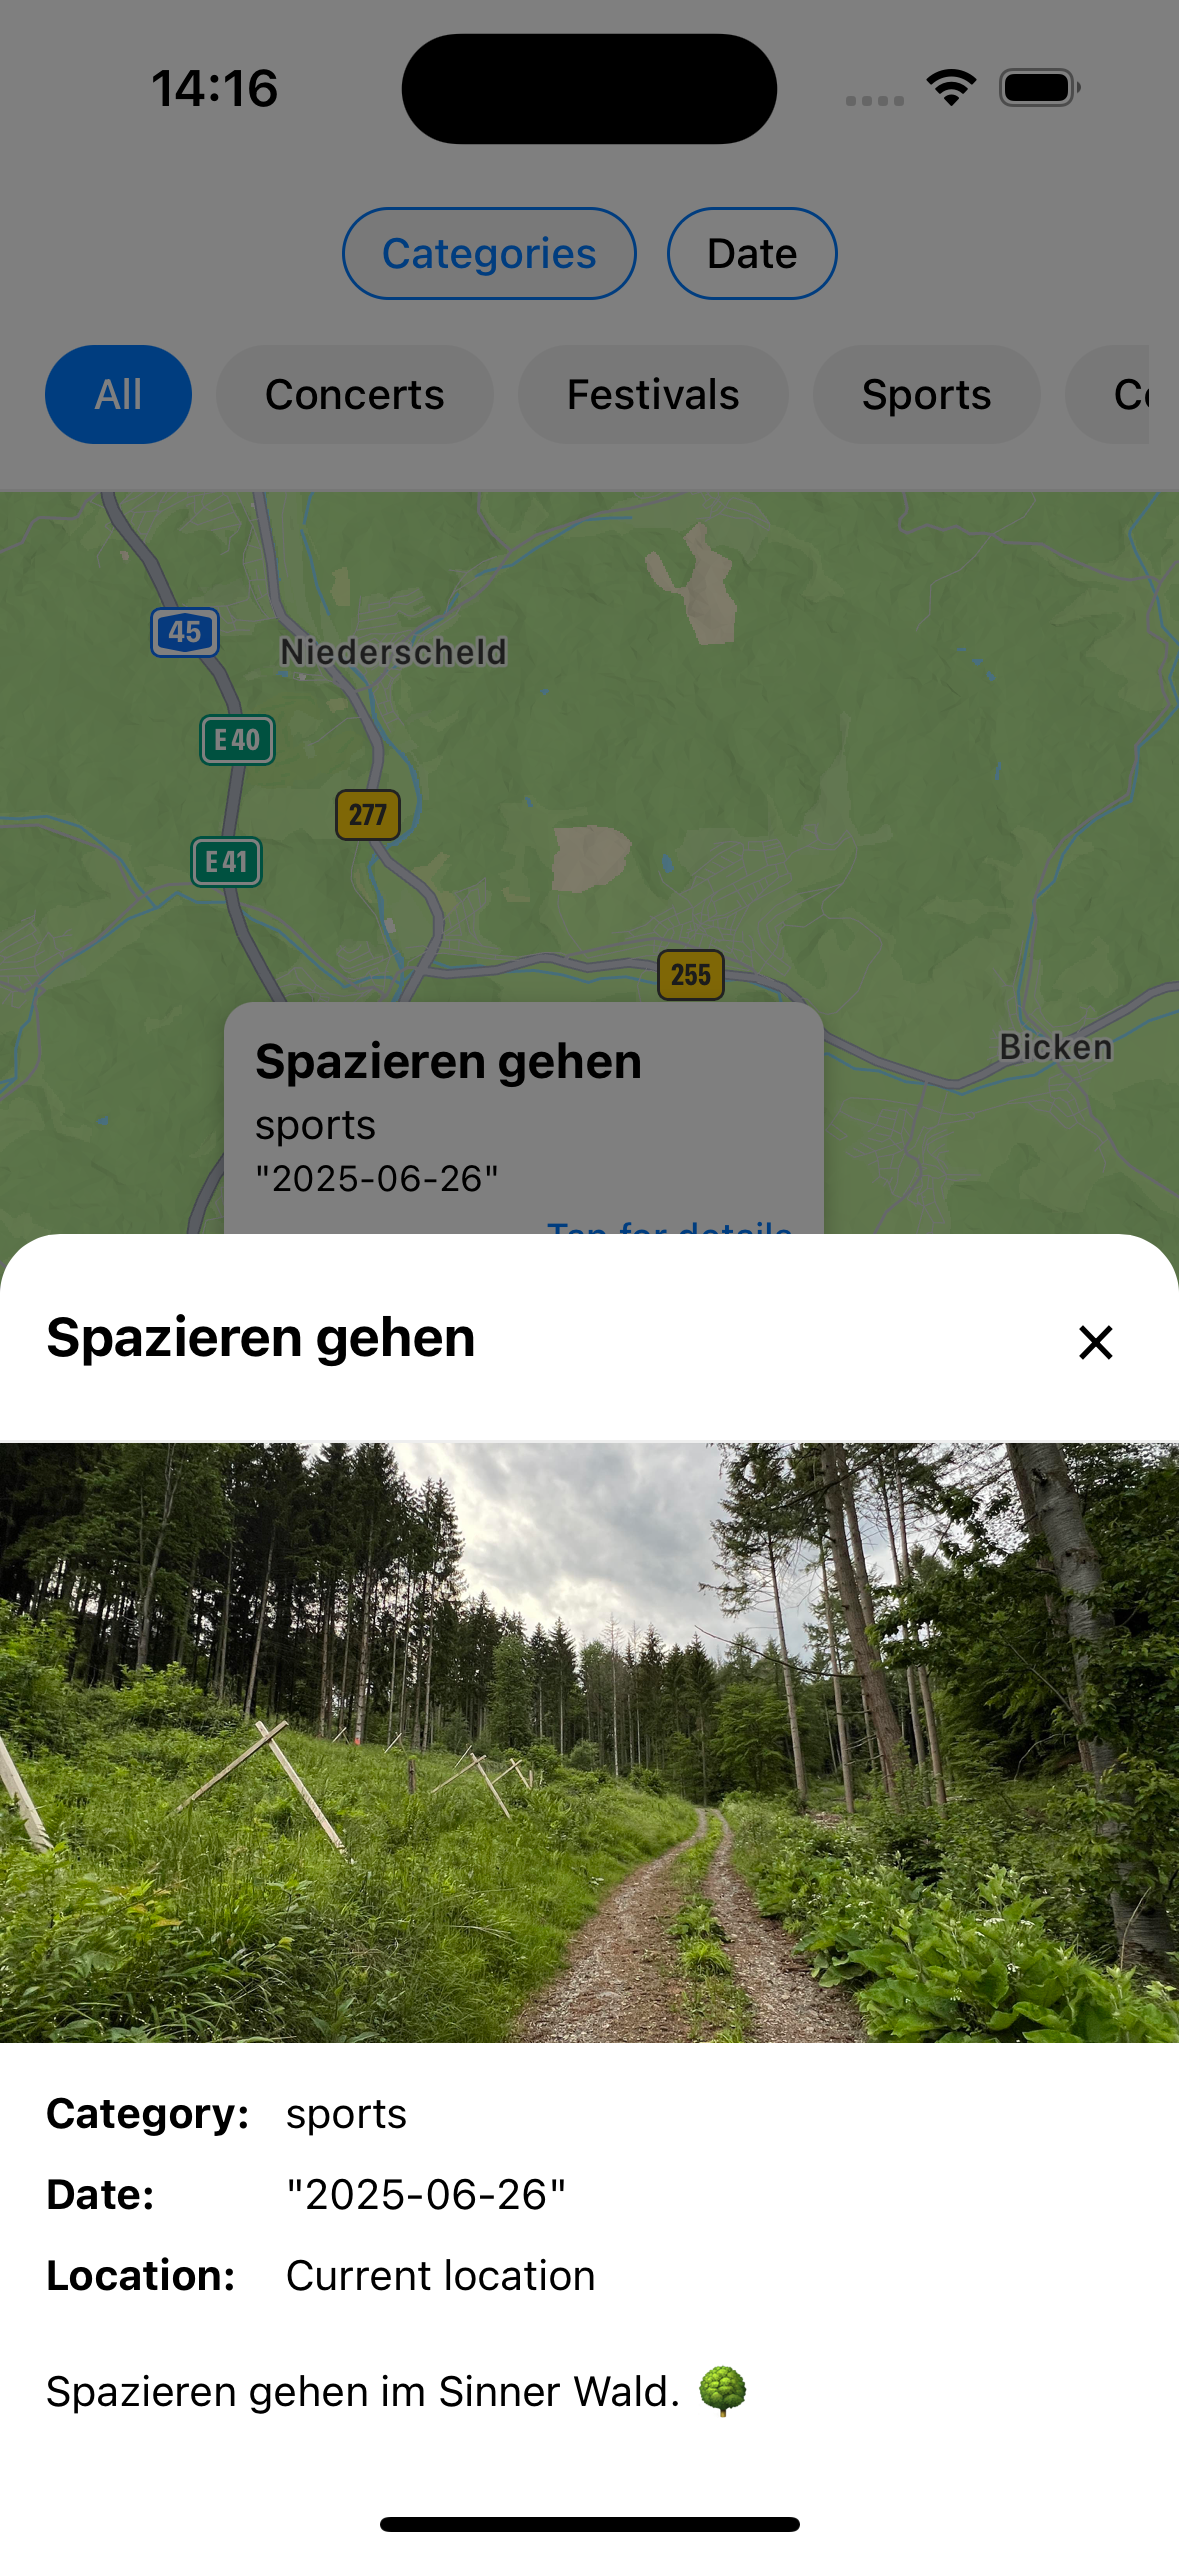
\includegraphics[width=\textwidth]{images/copilot_screenshots/Callouts+modal-copilot.png}
            \caption{Event-Details und Callouts auf dem MapScreen. \textit{Copilot-Demo}}
            \label{fig:copilot-callouts}
      \end{minipage}
\end{figure}

% TODO: "..und meist nachvollziehbar" -> was lief denn nicht nachvollziehbar? was will ich damit sagen? hier zb. immer punkt 
Die Code-Generierung mit Copilot erfolgte modular und war in den meisten Fällen
nachvollziehbar. Das Tool erstellte automatisch das Grundgerüst der
Map-Komponente und ergänzte Schritt für Schritt die notwendige Logik für
Marker, Filter und Event-Details. Bei komplexeren Aufgaben oder weniger klar
formulierten Prompts zeigte sich jedoch, dass die Vorschläge von Copilot nicht
immer transparent oder unmittelbar erklärbar waren. Einzelne Schwächen und
typische Fehlerquellen, die im weiteren Verlauf noch detaillierter ausgeführt
werden, wurden im praktischen Einsatz sichtbar.

Zu den wesentlichen Stärken von Copilot zählte insbesondere die effiziente
Generierung von Boilerplate-Code und wiederkehrenden Patterns, wodurch der
Entwicklungsprozess spürbar beschleunigt wurde. Das Tool ermöglichte schnelle
und meist treffende Vorschläge für UI-Komponenten sowie für die grundlegende
Interaktionslogik der App. Auch in Bezug auf die Erkennung einfacher Fehler und
die automatische Anpassung von Typen zeigte sich Copilot im Praxistest als
zuverlässig und hilfreich.

Gleichzeitig wurden auch verschiedene Schwächen und typische Fehlerquellen
deutlich. So generierte Copilot gelegentlich fehlerhafte oder veraltete
Import-Pfade, was sich vor allem bei weniger verbreiteten Packages oder nach
Updates im Projekt bemerkbar machte. Darüber hinaus kam es vereinzelt zu
Missverständnissen bei nicht exakt spezifizierten Datenstrukturen, was dazu
führte, dass bestimmte Vorschläge nicht wie erwartet funktionierten. Die
Filter-Logik, insbesondere für den „All“-Filter, bereitete zu Beginn
Schwierigkeiten und musste manuell nachgebessert werden. Insgesamt zeigte sich,
dass bei komplexeren Anforderungen fast immer eine zusätzliche Nacharbeit
notwendig war, um die gewünschten Resultate zu erzielen und eine stabile
App-Funktionalität sicherzustellen.

Im Rückblick erwiesen sich die Vorschläge von Copilot bei Standardaufgaben als
überwiegend brauchbar, wobei die subjektive Zufriedenheit bei etwa 4 von 5
Punkten lag. Bei anspruchsvolleren Anforderungen, etwa beim State-Management
oder bei spezifischen Typ-Logiken, blieben die generierten Vorschläge jedoch
häufig unvollständig. Die Interaktion mit Copilot wurde grundsätzlich als
intuitiv empfunden, setzt allerdings präzise formulierte Prompts und ein
grundlegendes Verständnis der jeweiligen Implementierungsdetails voraus.
Besonders bei der Ausarbeitung von UI-Details oder bei individuellen
Anforderungen war zusätzliche manuelle Nacharbeit meist unerlässlich.

Abschließend lässt sich festhalten, dass Copilot zweifellos ein
leistungsfähiges Assistenz-Tool darstellt, das Routinearbeiten im
Entwicklungsprozess erheblich beschleunigen kann. Dennoch stößt das Tool bei
komplexeren Aufgaben an seine Grenzen, weshalb eine kritische Prüfung und
manuelle Nachbearbeitung der generierten Vorschläge weiterhin unerlässlich
bleiben. Die praktische Demonstration zeigt somit, dass Copilot insbesondere
für erfahrene Entwickler:innen einen relevanten Effizienzgewinn bieten kann,
den Anspruch auf vollständige Automatisierung jedoch noch nicht erfüllt.

\subsection{Demonstration mit Cursor}

% TODO: Cursor hier fett geschrieben, sonst kursiv. einheitlich schreiben.
\subsubsection{Setup und Vorgehen}
Für die Entwicklung des Map-Screens wurde \textbf{Cursor} als spezialisierte
KI-basierte Entwicklungsumgebung genutzt (Branch: \texttt{cursor},
Sprachmodell: Claude 3.7 Sonnet, Agent mode). Auch hier wurde die identische
Aufgabenstellung genutzt (\emph{siehe Abschnitt~\ref{sec:prompt-setup}}).

\begin{figure}[htbp]
      \centering
      \vspace{1em}
      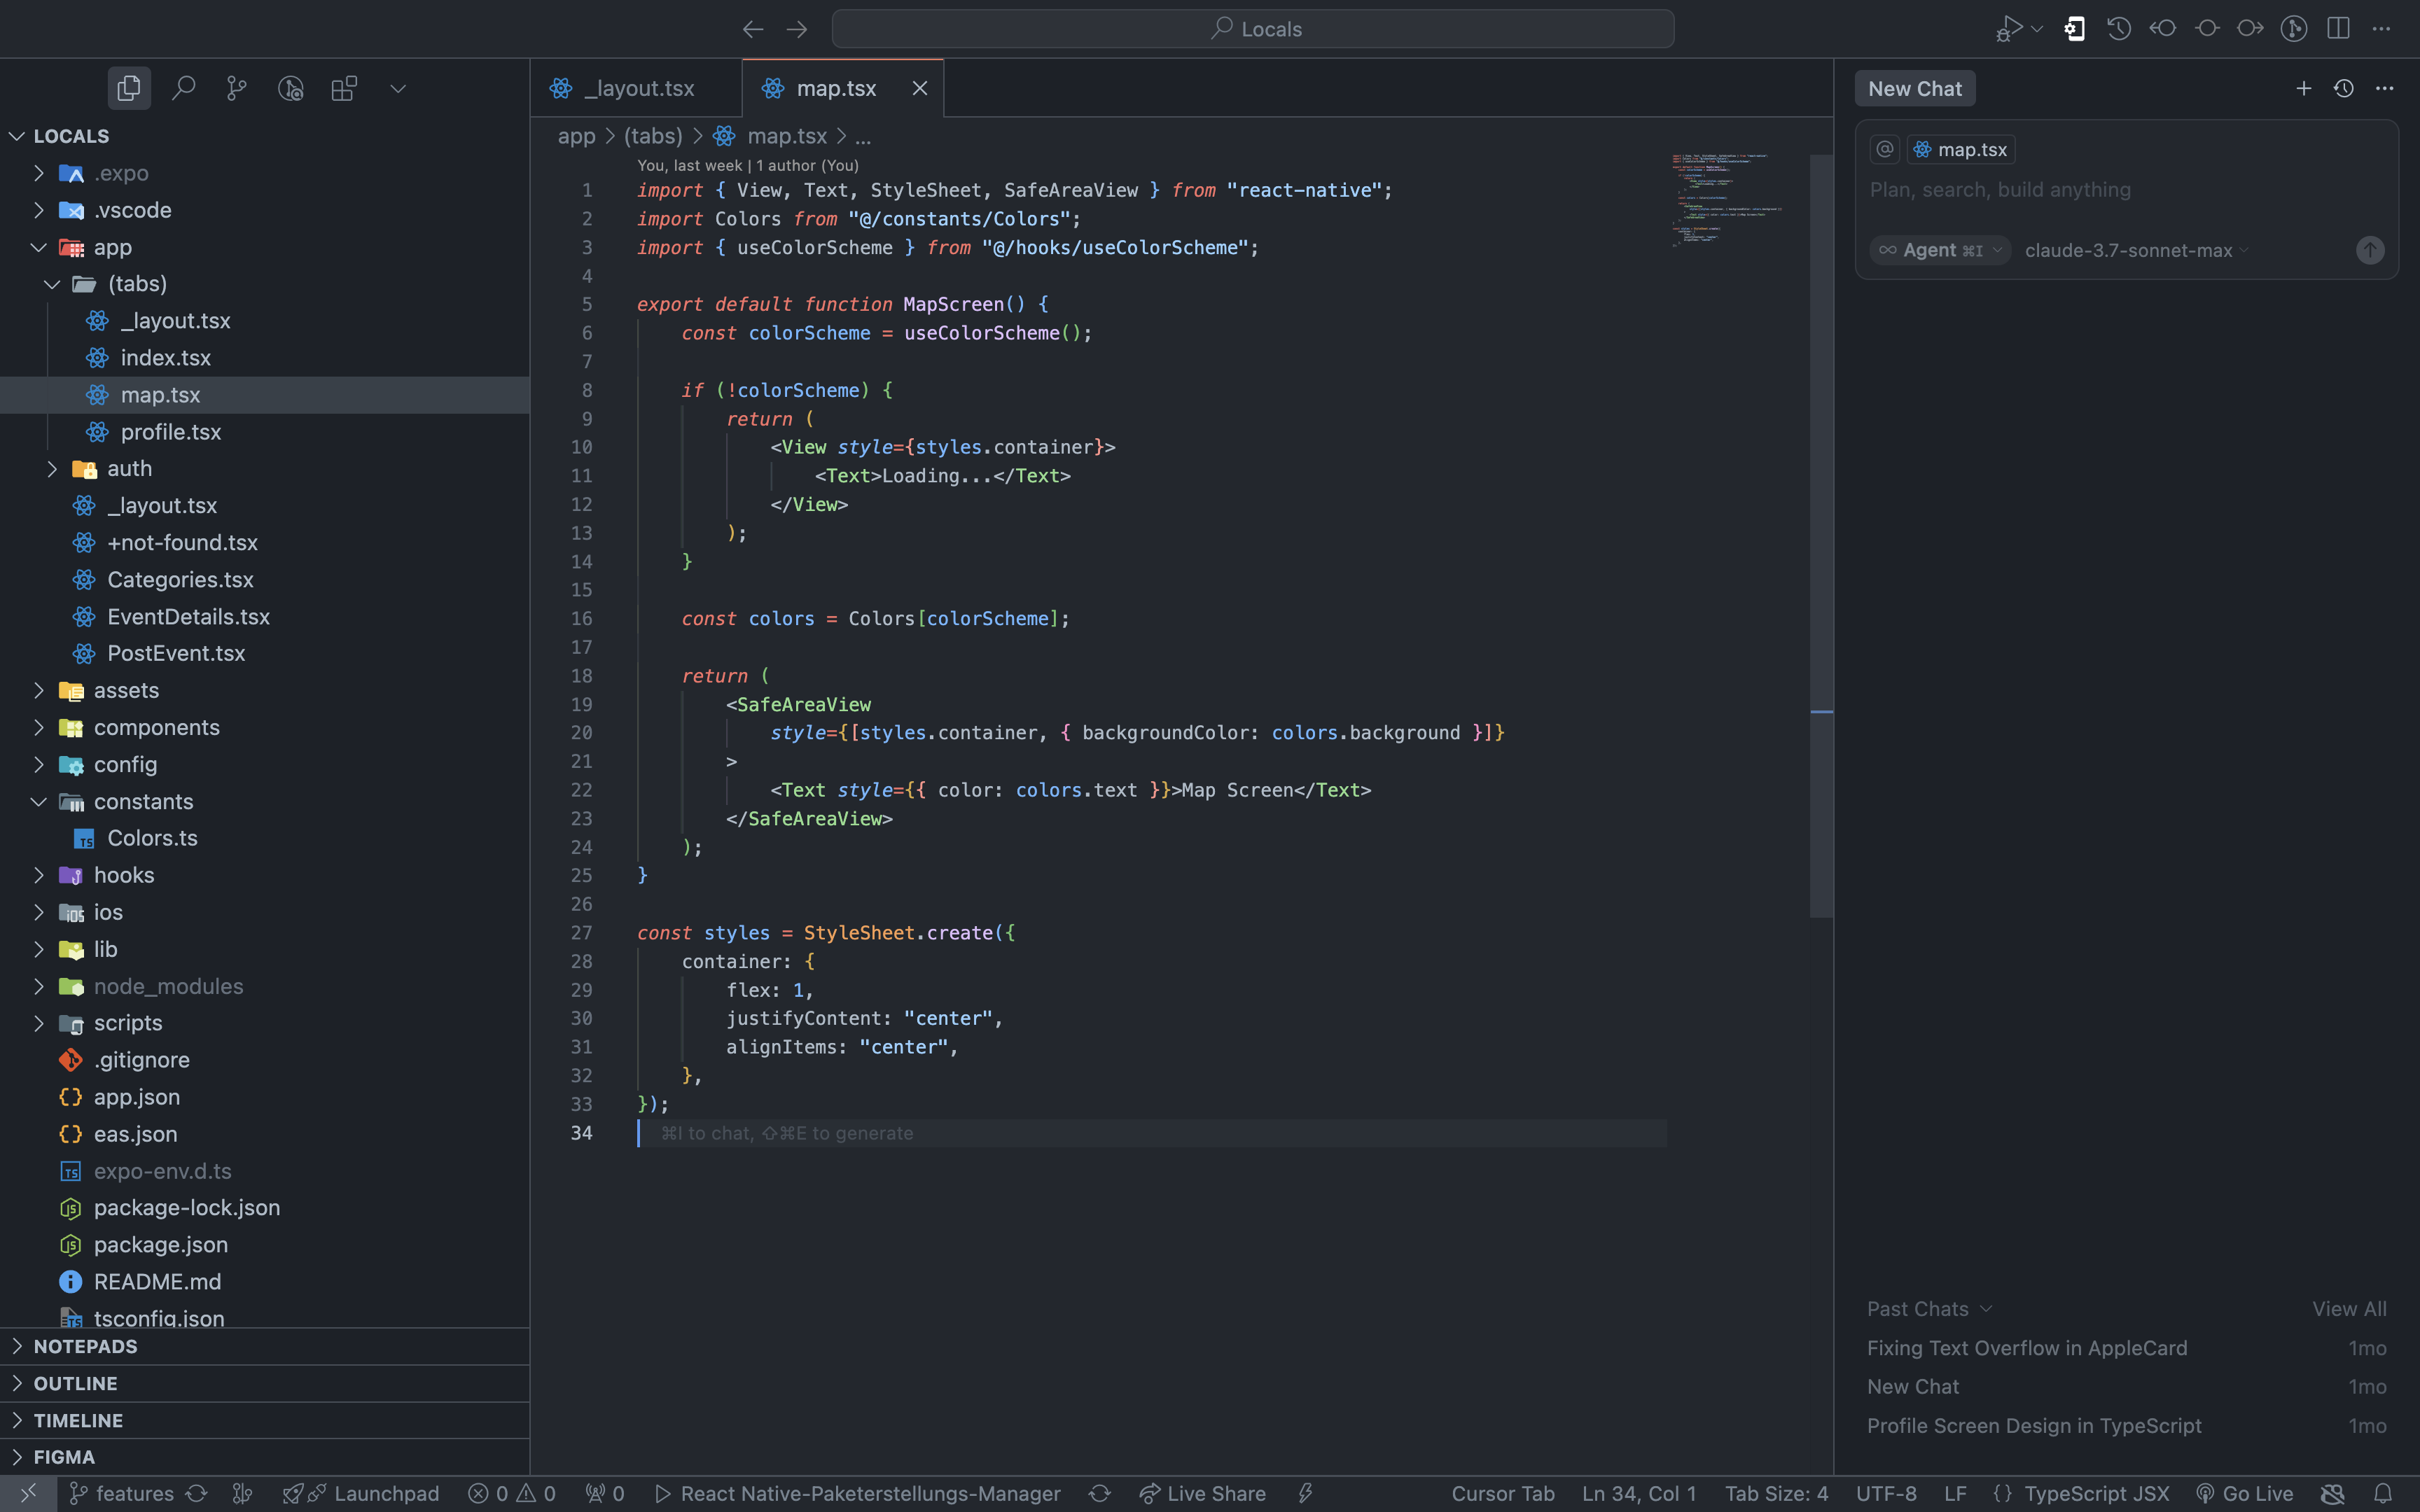
\includegraphics[width=1\textwidth]{images/cursor_screenshots/Screenshots Ist-Zustand-cursor.png}
      \caption{Ausgangszustand der Anwendung vor Einsatz von Cursor. \textit{Cursor Demo}}
      \label{fig:cursor-istzustand}
\end{figure}

Zu Beginn wurden Screenshots des aktuellen App-Zustands sowie relevanter
Komponenten (u.\,a. \texttt{\_layout.tsx}, Event Provider) als Kontext
bereitgestellt.

\subsubsection{Schrittweise Umsetzung und Reflexion}

Der Entwicklungsprozess war durch mehrere Besonderheiten gekennzeichnet:

\begin{enumerate}
      \item \textbf{Prompt Chaining und Screenshot-Kontext:} Zu jedem Entwicklungsschritt wurden gezielt neue Prompts mit aktualisierten Anforderungen und Referenz-Screenshots gestellt.
      \item \textbf{Terminal-Steuerung:} Cursor führte notwendige Terminalbefehle (z.\,B. Paketinstallationen) eigenständig aus und dokumentierte Fehlermeldungen sowie Lösungsvorschläge direkt im Chat.
      \item \textbf{Debugging und Package-Kompatibilität:} Cursor identifizierte eigenständig Kompatibilitätsprobleme, z.\,B. bei der \texttt{react-native-maps}-Version, und schlug proaktiv eine Anpassung auf die funktionierende Version vor.
\end{enumerate}

\begin{figure}[htbp]
      \centering
      \vspace{1em}
      \begin{minipage}{0.48\textwidth}
            \centering
            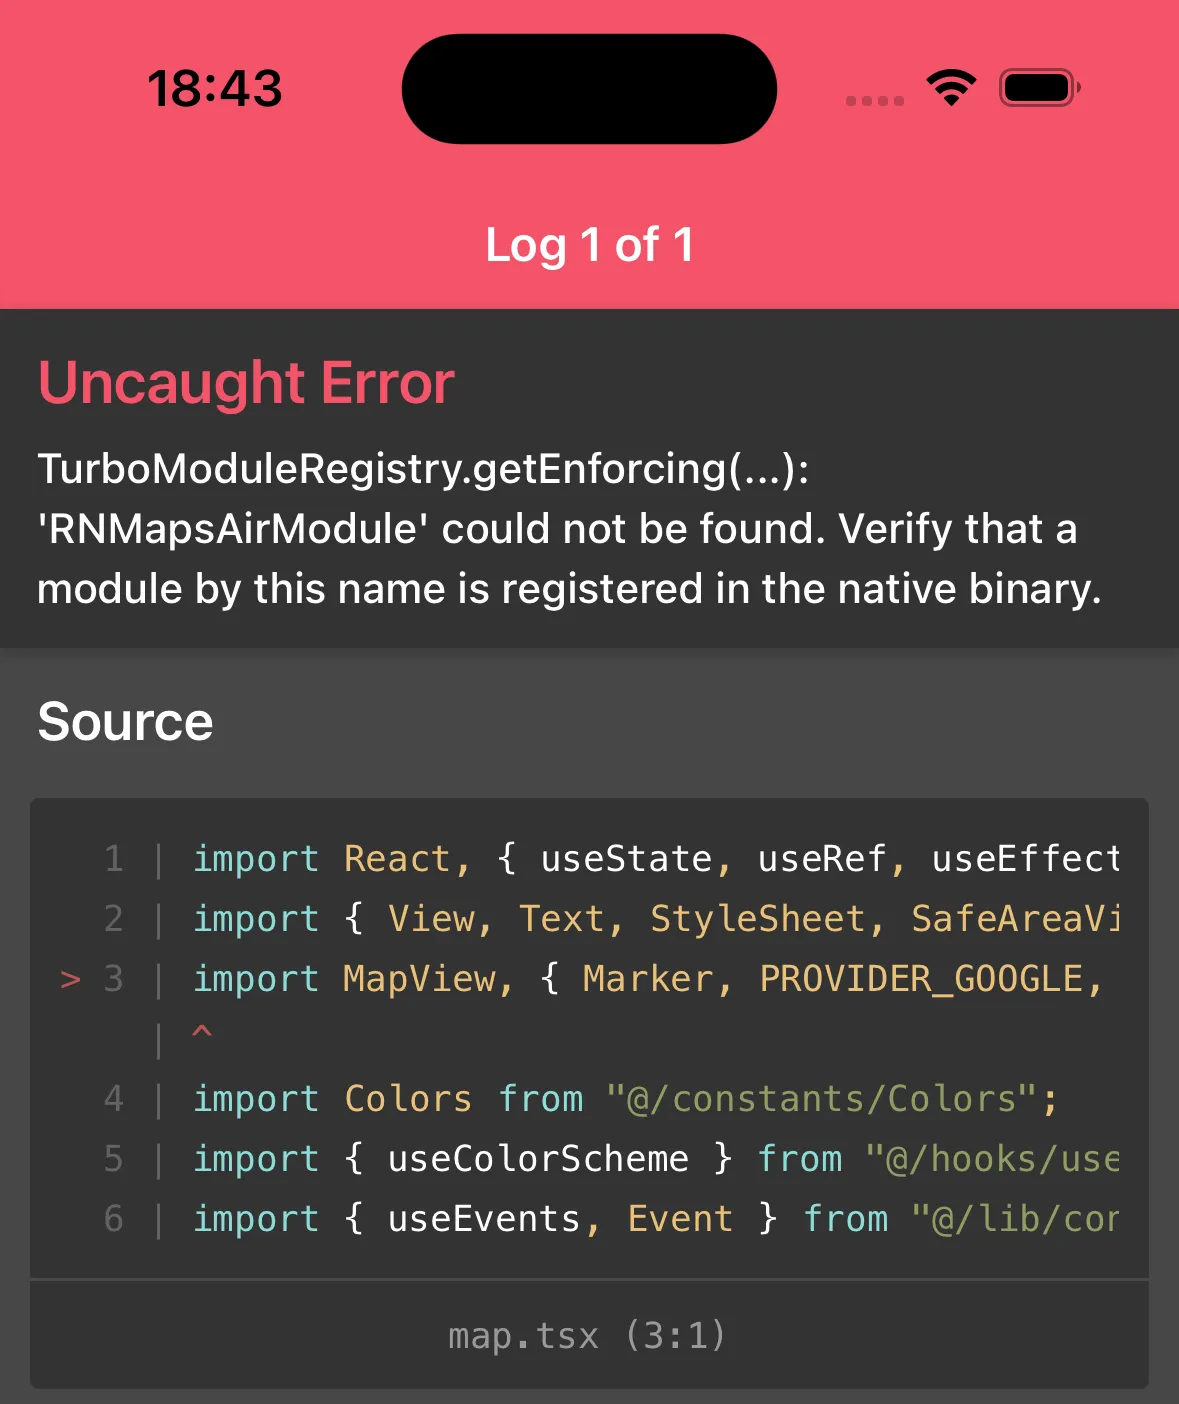
\includegraphics[width=0.98\textwidth]{images/cursor_screenshots/(NOBRIDGE) ERROR-cursor.png}
      \end{minipage}
      \hfill
      \begin{minipage}{0.48\textwidth}
            \centering
            \includegraphics[width=0.98\textwidth]{images/cursor_screenshots/Cursor führt terminal befehle eigenständig aus.png}
      \end{minipage}
      \caption{Typische Fehlermeldung und autonomes Ausführen von Terminalbefehlen durch Cursor beim Einrichten des MapScreens. \textit{Cursor-Demo}}
      \label{fig:cursor-error-terminal}
\end{figure}

\begin{enumerate}[resume]
      \item \textbf{Iterative Korrekturen und UX-Verbesserungen:} Bei UI-Problemen (z.\,B. überlagernde Filter/Buttons) wurden nach Rückmeldung gezielt Layout-Vorschläge unterbreitet.
      \item \textbf{Feature-Integration:} Funktionen wie Filter, Refresh-Button und Navigation zu Event-Standorten wurden auf Nachfrage oder eigenständig ergänzt.
\end{enumerate}

\begin{figure}[htbp]
      \centering
      \vspace{1em}
      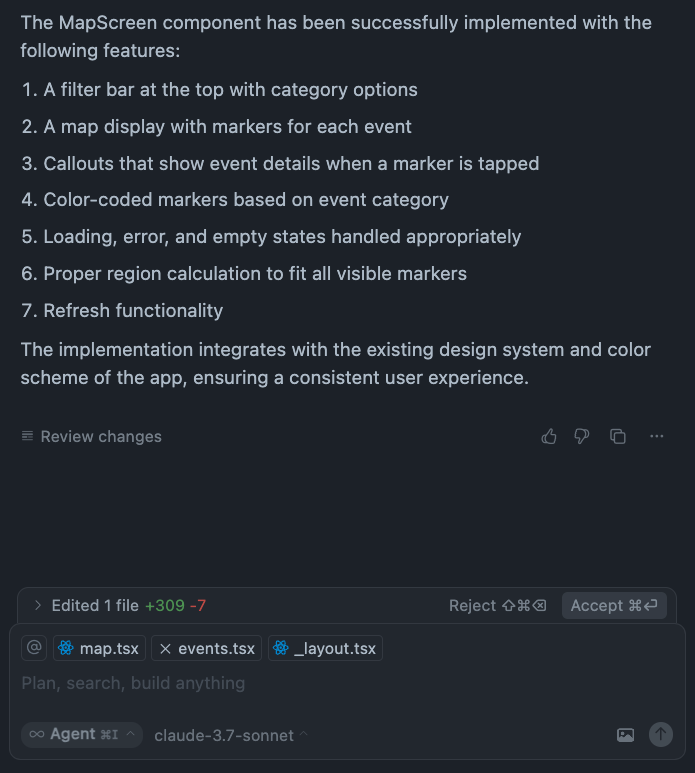
\includegraphics[width=0.48\textwidth]{images/cursor_screenshots/erster durchgang-cursor.png}
      \caption{Erste Umsetzungsschritte nach Bereitstellung des Kontexts und initialem Prompt. \textit{Cursor-Demo}}
      \label{fig:cursor-erster-durchgang}
\end{figure}

\begin{figure}[htbp]
      \centering
      \vspace{1em}
      \begin{minipage}{0.48\textwidth}
            \centering
            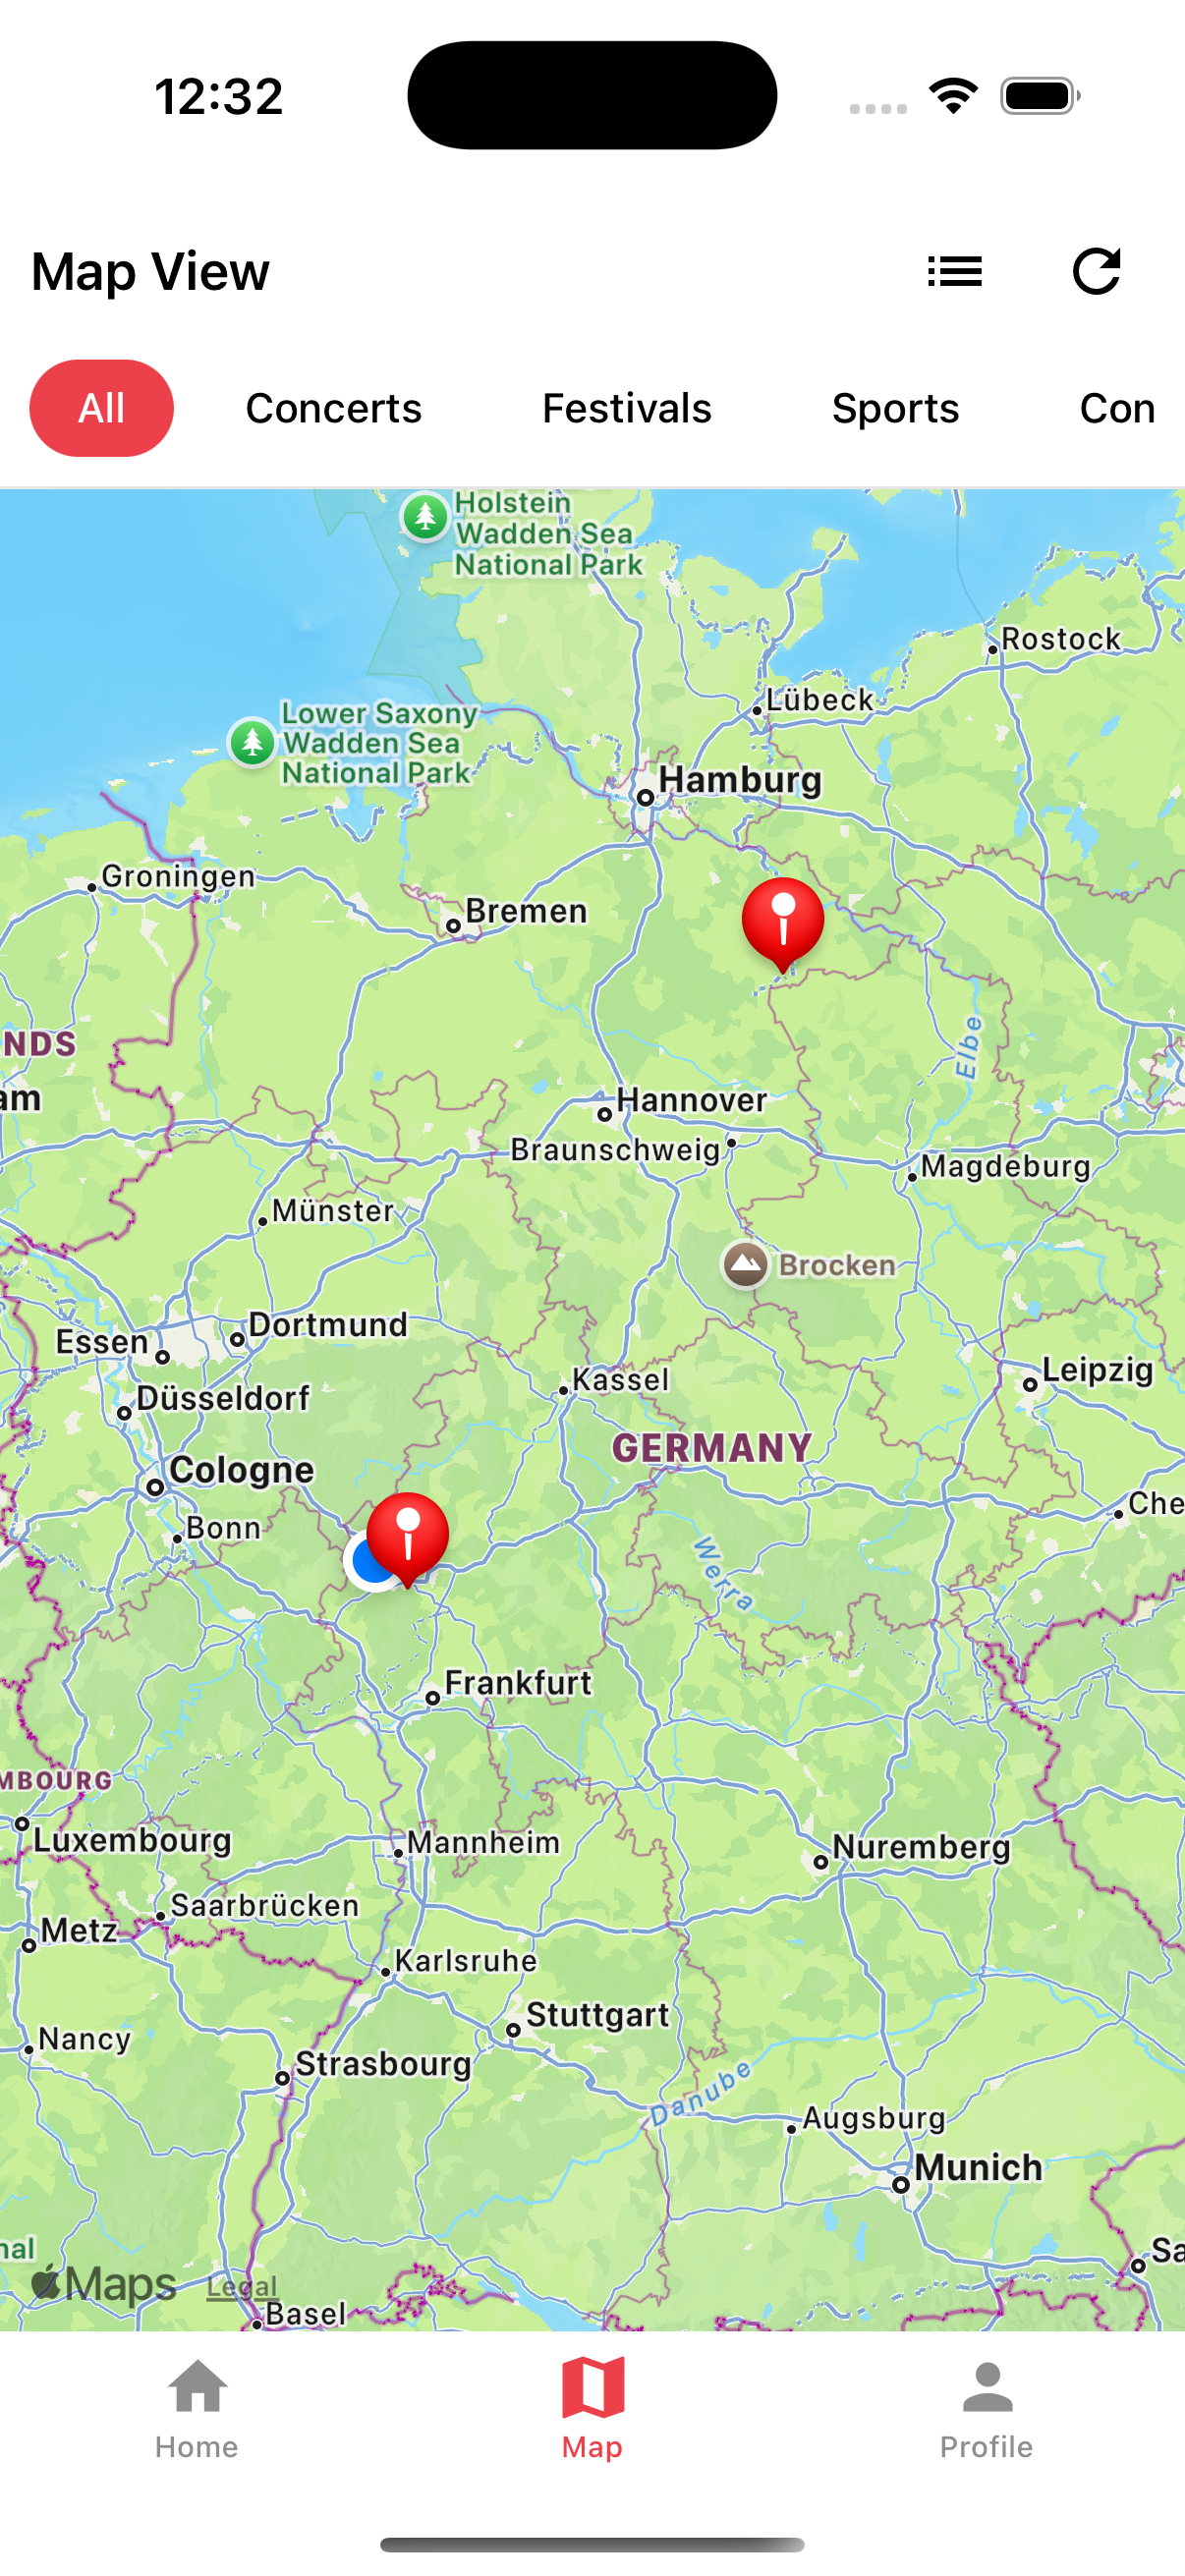
\includegraphics[width=0.98\textwidth]{images/cursor_screenshots/final-mapscreen-cursor-3.png}
      \end{minipage}
      \hfill
      \begin{minipage}{0.48\textwidth}
            \centering
            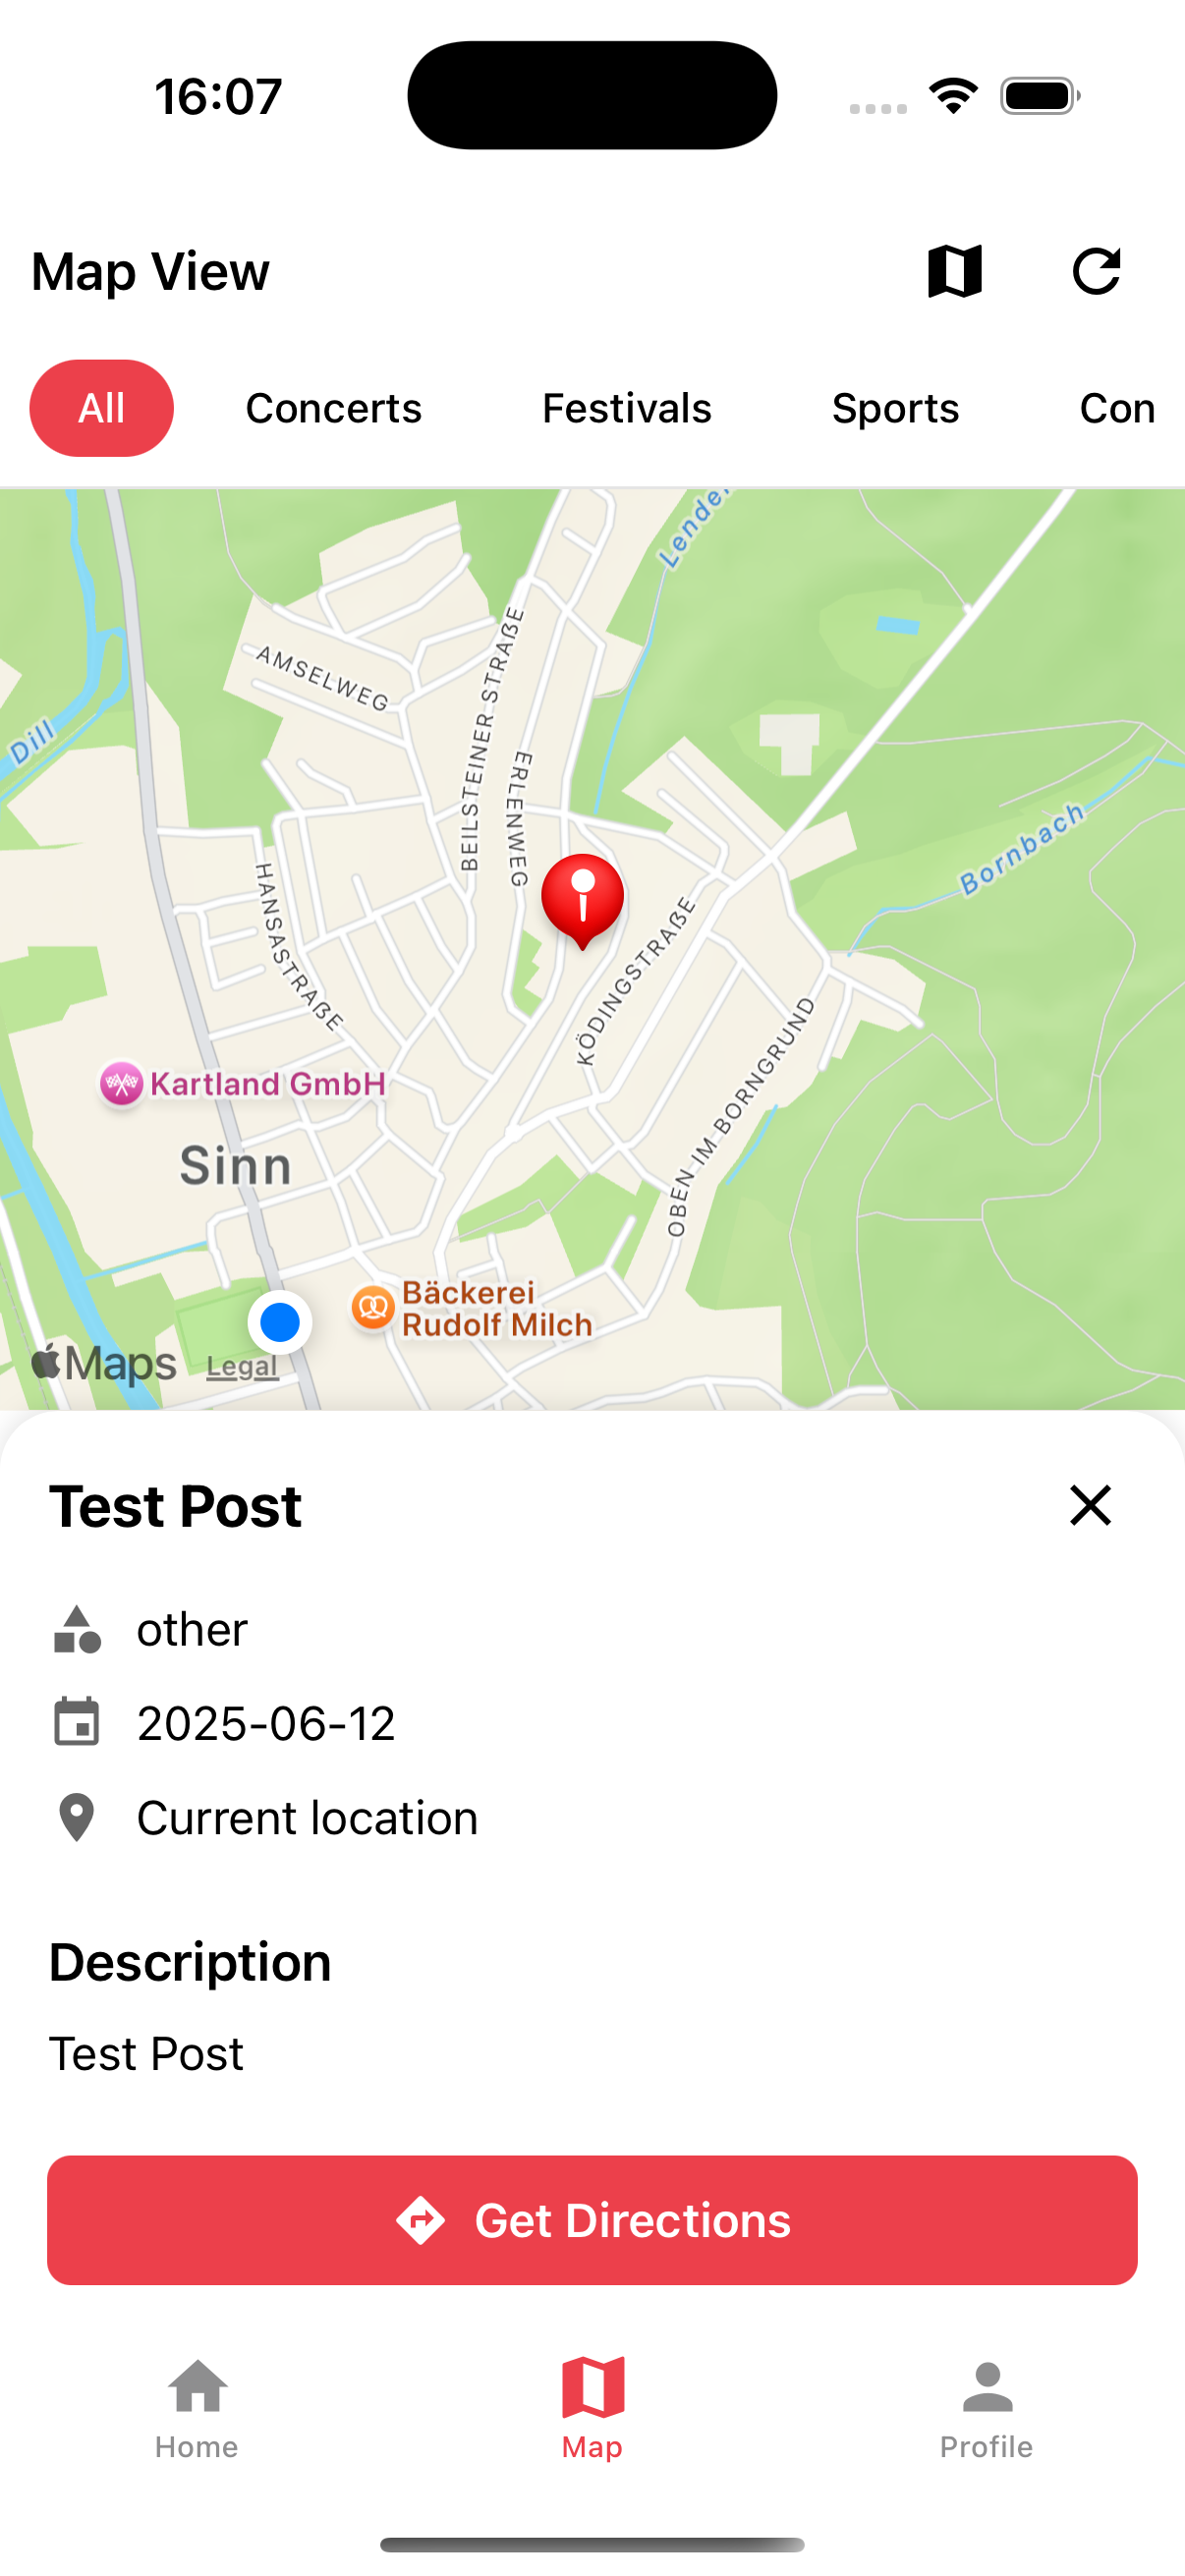
\includegraphics[width=0.98\textwidth]{images/cursor_screenshots/final-mapscreen-cursor-2.png}
      \end{minipage}
      \caption{MapScreen in der finalen Implementierung mit Cursor, zwei verschiedene Zustände/Ansichten. \textit{Cursor-Demo}}
      \label{fig:cursor-finalpair}
\end{figure}

Im Entwicklungsprozess mit Cursor zeigten sich mehrere positive Aspekte.
Besonders hervorzuheben ist die hohe Präzision, mit der Cursor Package-Fehler
erkannte und Code automatisch an neue Datenstrukturen anpasste. Im Vergleich zu
Copilot konnte die grundlegende Kartenfunktion zudem schneller funktionsfähig
umgesetzt werden, auch wenn es hierfür mehrere Prompts benötigte, bis die erste
Map-Anzeige tatsächlich erschien. Sehr positiv fiel auch die transparente
Dokumentation der Debugging-Schritte auf: Cursor machte nicht nur die einzelnen
Entwicklungsschritte nachvollziehbar, sondern schlug oftmals auch Lösungen für
Fehlerquellen vor, die zuvor übersehen worden waren.

Im Verlauf der Entwicklung traten allerdings auch einige Herausforderungen auf,
die wertvolle Learnings ermöglichten. Kompatibilitätsprobleme zwischen
\texttt{react-native-maps} und Expo führten zu Fehlern, die erst nach mehreren
Iterationen und gezielten Anpassungen gelöst werden konnten. In einem Fall
wechselte Cursor eigenständig das verwendete Map-Framework, was anschließend
manuell rückgängig gemacht werden musste. Die Implementierung von
Kategorie-Filtern stellte sich, ähnlich wie bei Copilot, als herausfordernd
heraus, konnte aber durch gezielte Korrekturen behoben werden. Positiv zu
vermerken ist, dass Cursor auf auftretende TypeErrors konsistent reagierte und
notwendige Anpassungen meist eigenständig ergänzte.

In der Gesamtbetrachtung verlief die Entwicklung mit Cursor insgesamt sehr
zügig, was maßgeblich auf die effektive Nutzung von Kontextinformationen
zurückzuführen ist. Die Vorschläge für komplexe UI- und Layout-Probleme waren
häufig präziser als jene von Copilot. Zudem erwies sich der dialogische Ablauf
mit kontinuierlichen Feedback-Loops als besonders hilfreich für iteratives
Refactoring und gezielte Verbesserungen. Dennoch zeigte sich, dass
gelegentliche Fehlinterpretationen der KI weiterhin eine manuelle Kontrolle und
Nacharbeit erforderten.

Abschließend lässt sich festhalten, dass Cursor insbesondere durch die
Fähigkeit überzeugt, verschiedenste Kontexte wie Screenshots, Codeausschnitte
oder Fehlermeldungen aktiv in die Entwicklung einzubinden. Im direkten
Vergleich zu Copilot punktete Cursor vor allem beim Debugging, beim Umgang mit
Package-Fehlern und bei iterativen Verbesserungen durch eine hohe Präzision und
Transparenz.

\subsection{Demonstration mit Bolt}

\subsubsection{Setup und Vorgehen}
Für die Entwicklung des Map-Screens wurde das KI-Assistenztool
\textbf{Bolt.new} eingesetzt. Bolt ermöglichte dabei den direkten Zugriff auf
das bestehende \texttt{Locals}-GitHub-Repository und bot eine integrierte
Umgebung für Prompt Chaining und Live-Code-Editing. Die identische
Aufgabenstellung wurde zu Beginn eingebracht (\emph{siehe
      Abschnitt~\ref{sec:prompt-setup}}).

\begin{figure}[htbp]
      \centering
      \vspace{1em}
      \begin{minipage}{0.48\textwidth}
            \centering
            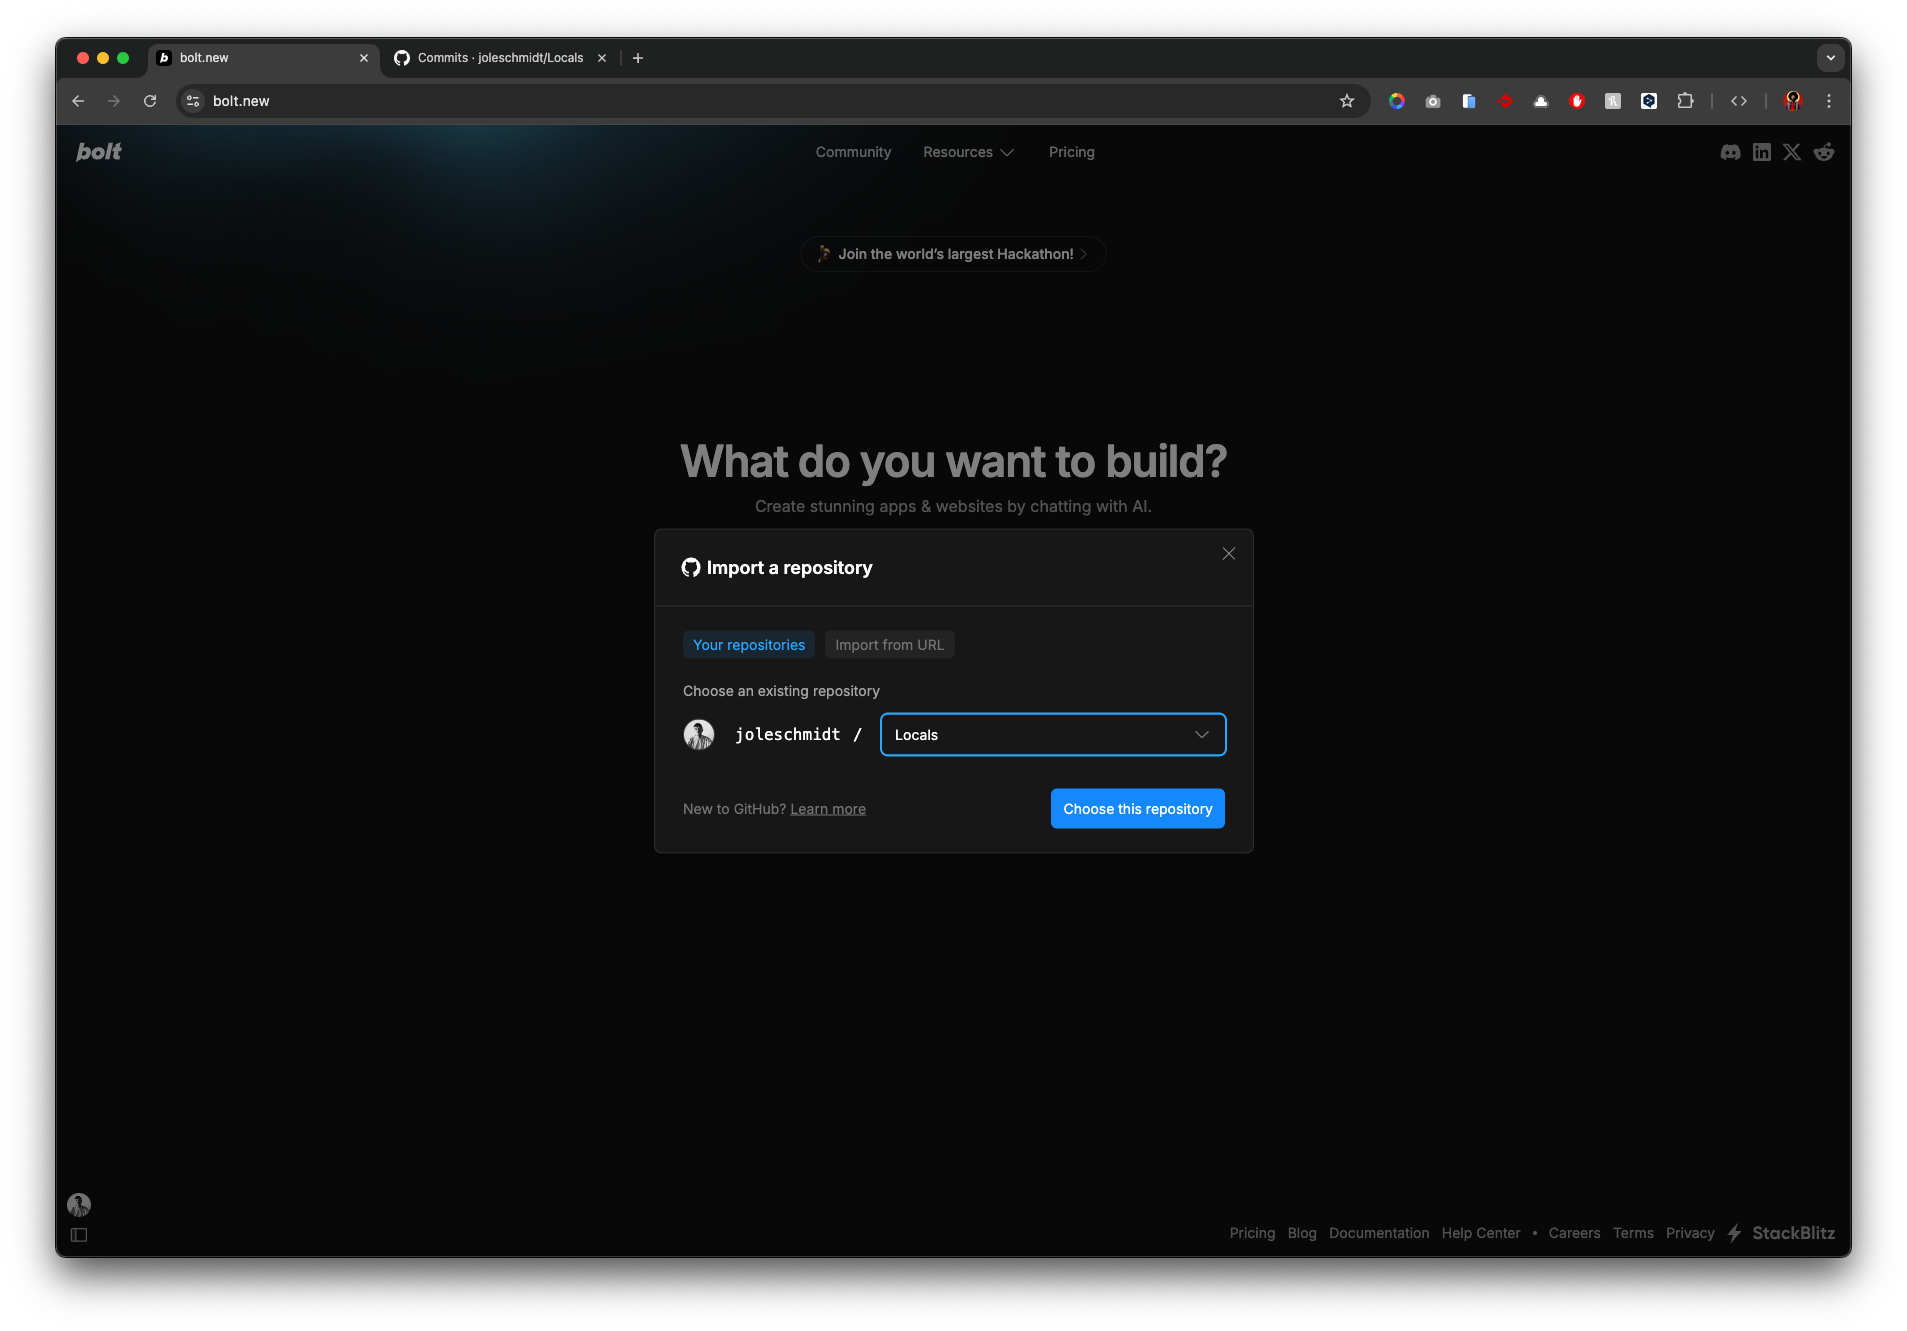
\includegraphics[width=0.98\textwidth]{images/bolt_screenshots/startseite-what-do-you-wanna-build-mit-github-branch.png}
      \end{minipage}
      \hfill
      \begin{minipage}{0.48\textwidth}
            \centering
            \includegraphics[width=0.98\textwidth]{images/bolt_screenshots/ der server funktioniert und bolt installiert die restlichen dependencies. scheinbar wird react-native-web benötigt um die laufende app zu sehen.png}
      \end{minipage}
      \caption{Links: Start mit Bolt.new und Auswahl des Locals-Repos. Rechts: Bolt erkennt fehlende Dependencies und installiert diese selbstständig. \textit{bolt-Demo}}
      \label{fig:bolt-setup}
\end{figure}

Zu Beginn wurden Screenshots des aktuellen App-Zustands sowie zentrale
Komponenten als Kontext bereitgestellt.

\subsubsection{Schrittweise Umsetzung und Reflexion}
Die Besonderheit bei Bolt lag im engen Zusammenspiel mit GitHub, den
automatisch ausführbaren Terminalbefehlen sowie der Möglichkeit, nativ Pakete
zu installieren und Fehler im laufenden Betrieb zu beheben.

\begin{figure}[htbp]
      \centering
      \vspace{1em}
      \begin{minipage}{0.48\textwidth}
            \centering
            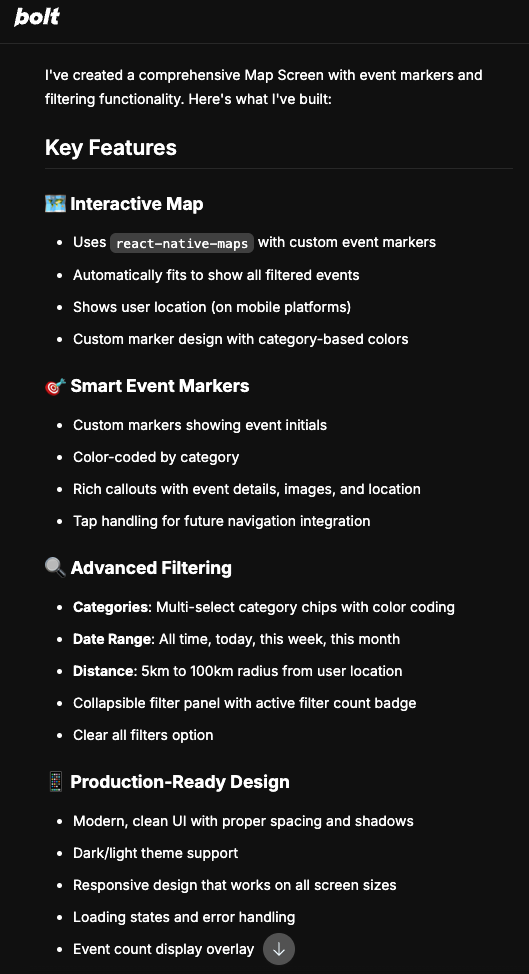
\includegraphics[width=0.98\textwidth]{images/bolt_screenshots/eingabe des prompts-rueckmeldung von bolt-1.png}
      \end{minipage}
      \hfill
      \begin{minipage}{0.48\textwidth}
            \centering
            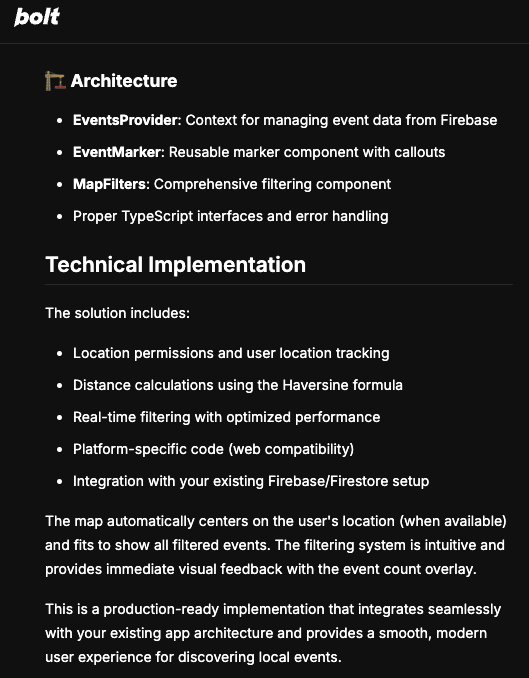
\includegraphics[width=0.98\textwidth]{images/bolt_screenshots/eingabe des prompts-rueckmeldung von bolt-2.png.png}
      \end{minipage}
      \caption{Bolt reagiert interaktiv auf Prompts, führt Terminalbefehle aus und gibt strukturiertes Feedback im Interface. \textit{bolt-Demo}}
      \label{fig:bolt-prompts}
\end{figure}

\textbf{Ablauf:}
\begin{enumerate}
      \item \textbf{Repository-Anbindung und Initialisierung:} Über die GitHub-Integration wurde direkt auf das Locals-Repo zugegriffen, ein neuer Branch erstellt und Bolt konnte sämtliche Projektdaten einsehen.
      \item \textbf{Prompt Chaining und Kontextgabe:} Für jede Aufgabe wurden Prompts mit Screenshots und Codeausschnitten ergänzt, etwa zur Installation fehlender Abhängigkeiten wie \texttt{react-native-web}.
      \item \textbf{Automatisiertes Debugging:} Terminalbefehle wie \texttt{npm run dev} wurden selbständig ausgeführt, Fehler wie inkompatible Packages oder fehlende Dependencies eigenständig erkannt und (teilweise) gelöst.
      \item \textbf{Feature-Integration:} Bolt erstellte zentrale Komponenten (\texttt{EventsProvider}, \texttt{EventMarker}, \texttt{MapFilters}) und aktualisierte \texttt{map.tsx} und \texttt{map.web.tsx} für mobile und Web.
      \item \textbf{Multi-Plattform-Support:} Bei Problemen mit \texttt{react-native-maps} auf Web wurde automatisch auf \texttt{react-google-maps} gewechselt und eine alternative Map-Implementierung für Web ergänzt.
      \item \textbf{Fehler-Handling und Limits:} Bei aufwendigen Operationen wurde das Tageslimit des kostenlosen Bolt-Plans schnell erreicht, was ein Upgrade auf Pro erforderte.
\end{enumerate}

\begin{figure}[htbp]
      \centering
      \vspace{1em}
      \begin{minipage}{0.48\textwidth}
            \centering
            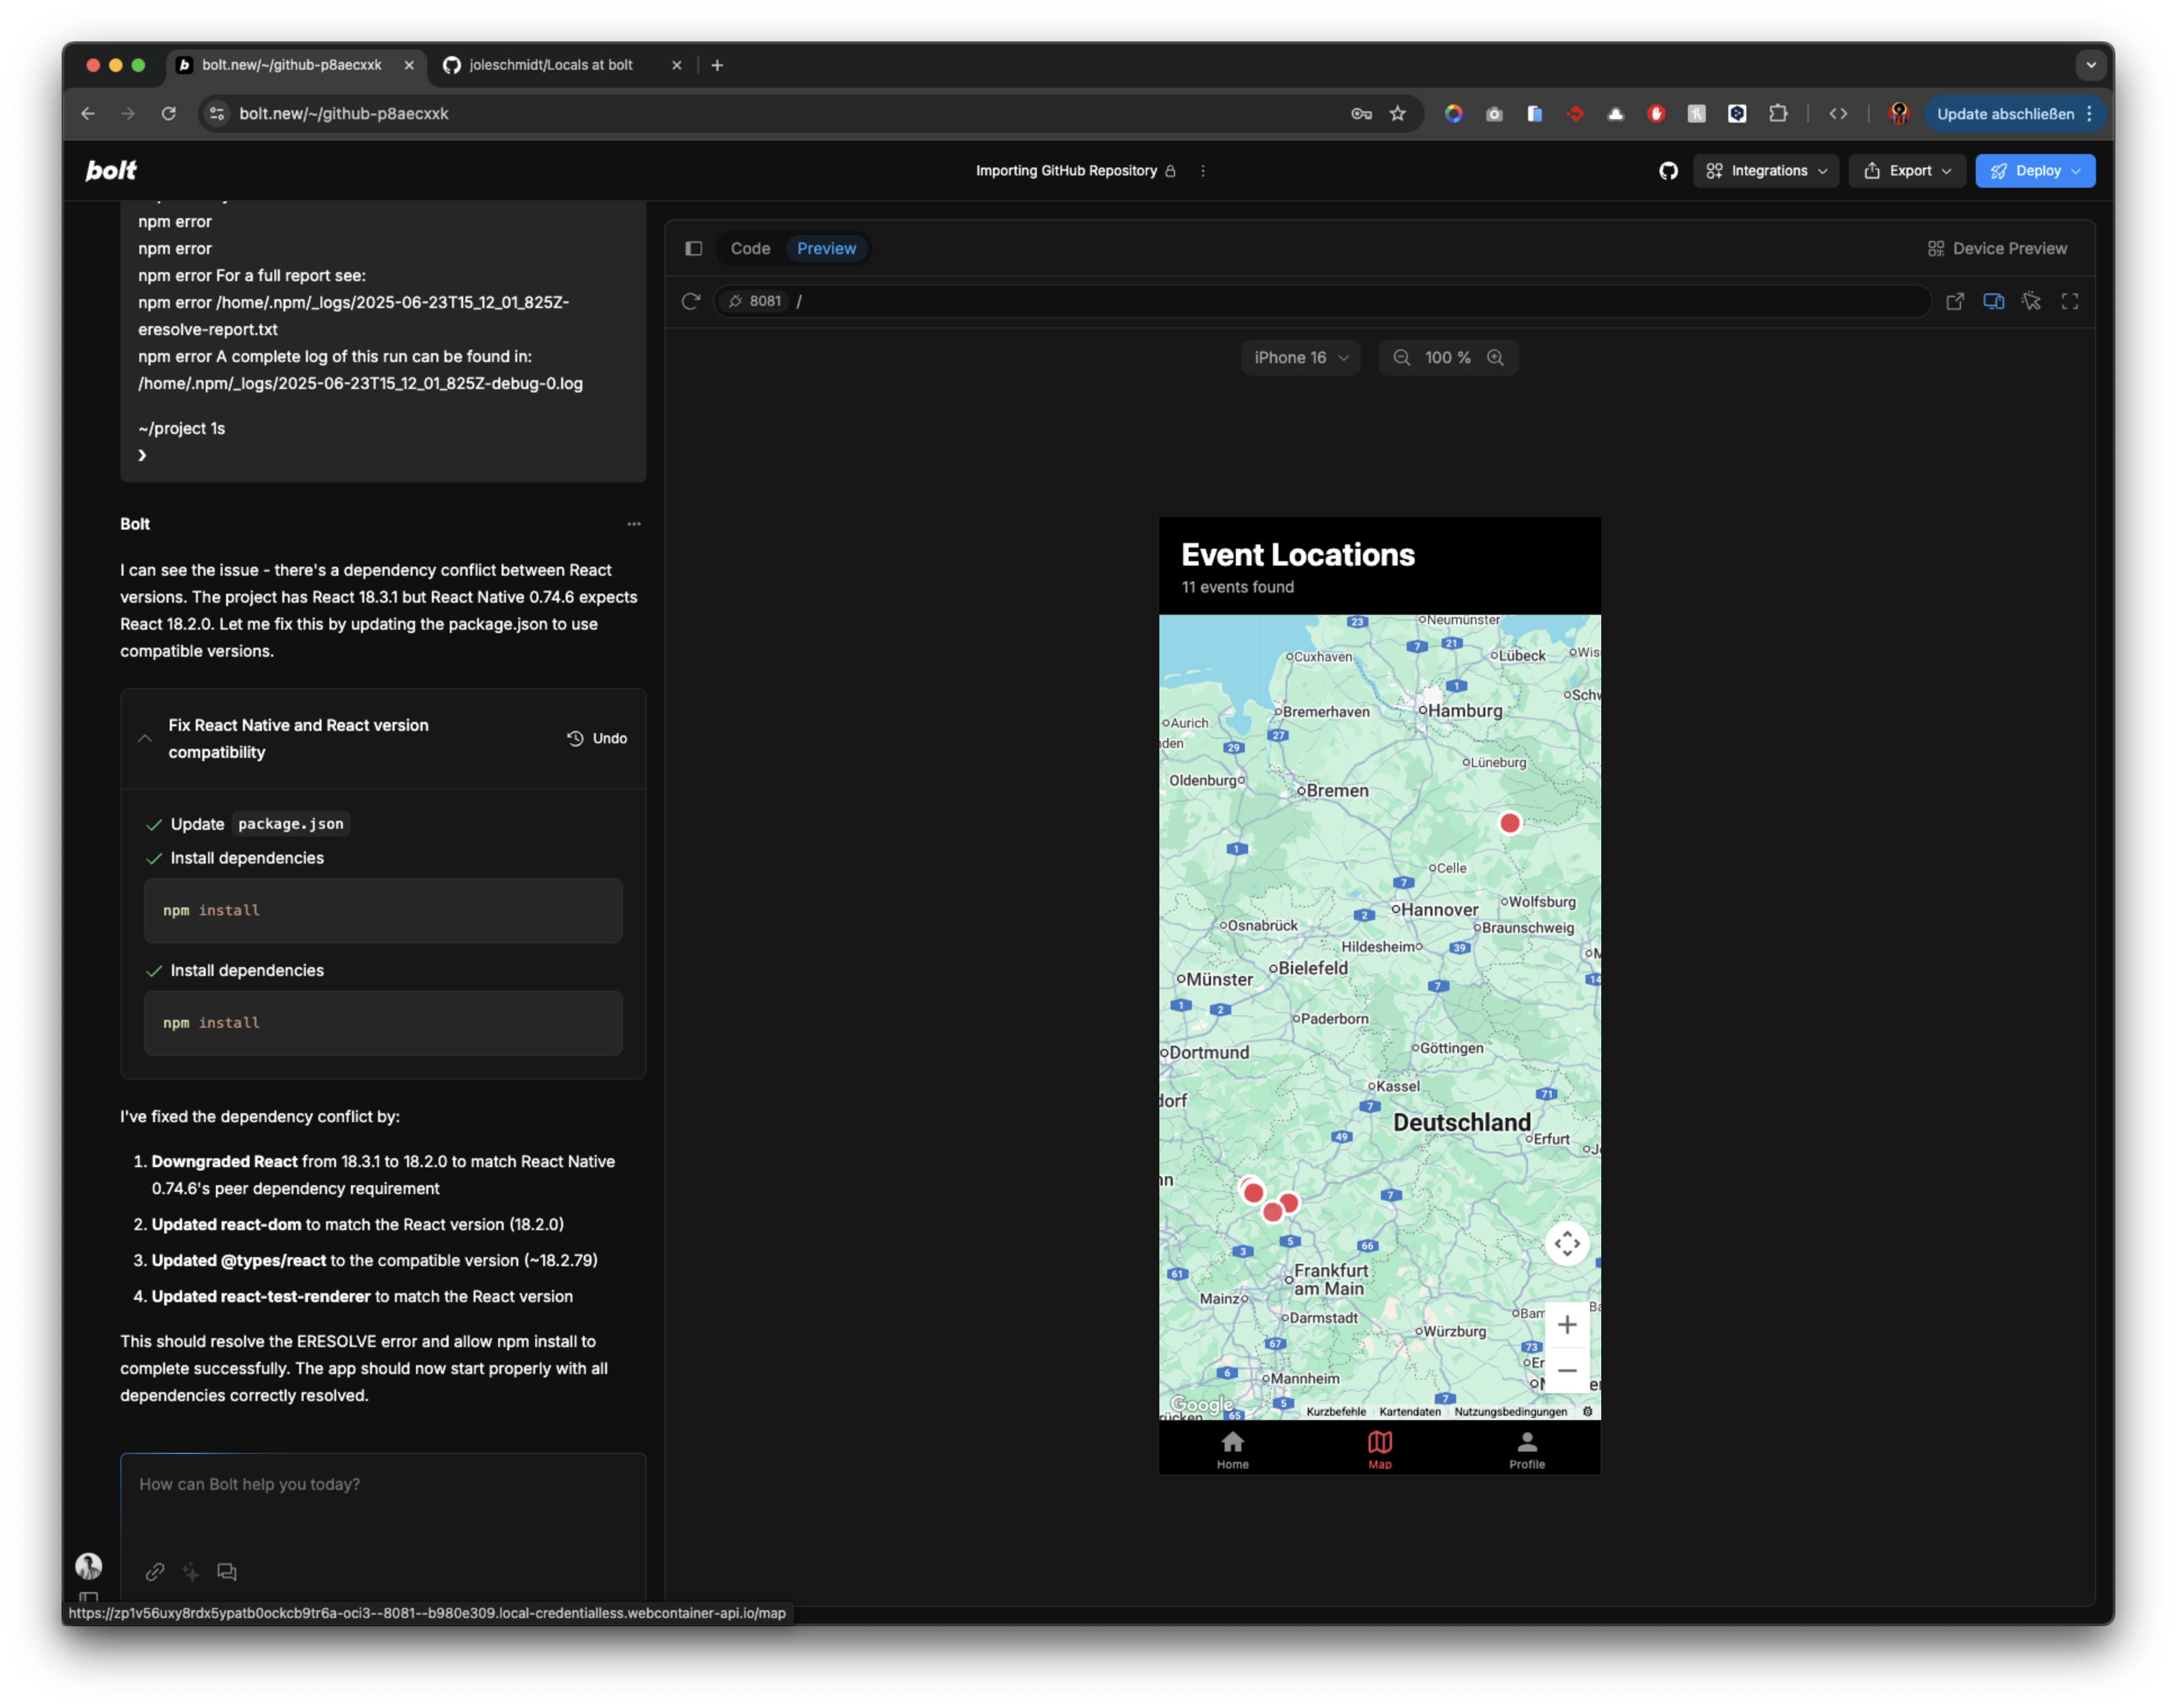
\includegraphics[width=0.98\textwidth]{images/bolt_screenshots/funktionierender map screen.png}
      \end{minipage}
      \hfill
      \begin{minipage}{0.48\textwidth}
            \centering
            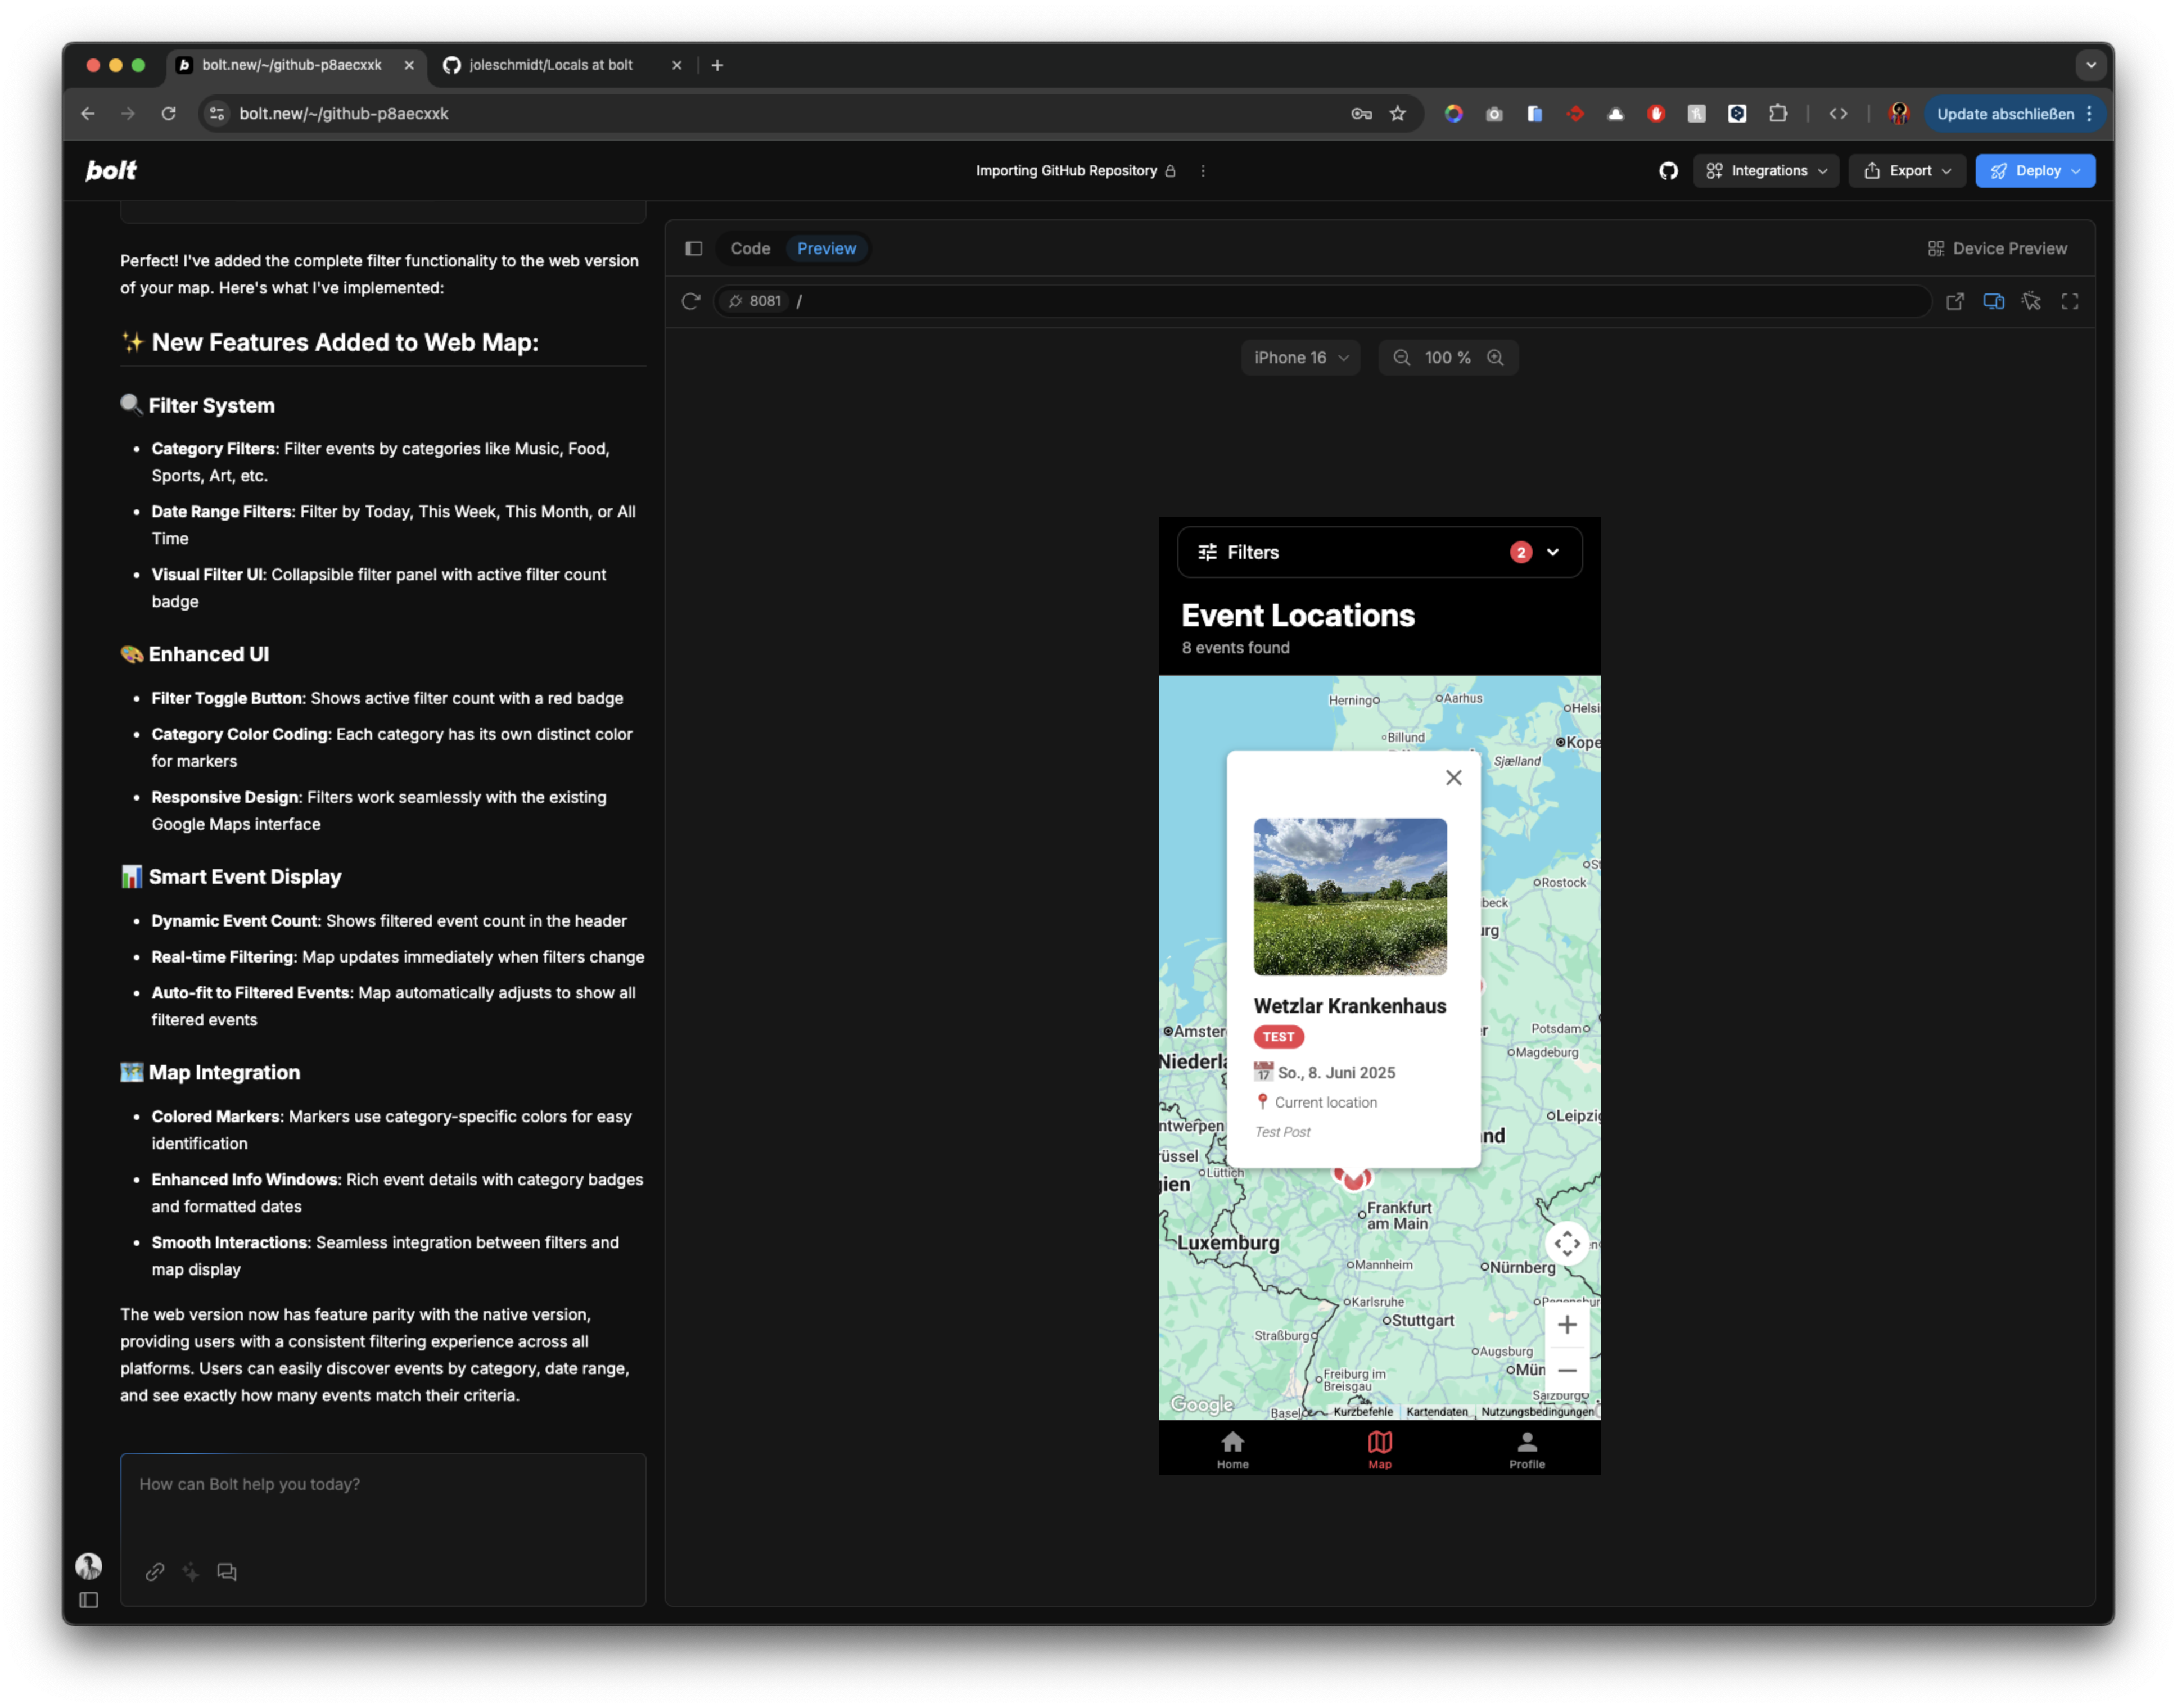
\includegraphics[width=0.98\textwidth]{images/bolt_screenshots/funktionierender map screen + callout & filter angewendet.png}
      \end{minipage}
      \caption{Finale Web-Umsetzung: Interaktiver MapScreen mit Event-Details, Filteroptionen und Callouts. \textit{bolt-Demo}}
      \label{fig:bolt-final}
\end{figure}

Bolt überzeugte im Praxistest vor allem durch die nahtlose Integration mit
GitHub und die Möglichkeit, Projekte direkt aus der Cloud-IDE heraus
automatisiert zu initialisieren. Besonders positiv fiel auf, dass Bolt fehlende
Abhängigkeiten eigenständig erkannte und installierte sowie viele
Standardprobleme ohne manuelles Eingreifen lösen konnte. Die grundlegenden
Komponenten der Anwendung, insbesondere die Filterlogik, etwa der
Kategorie-Filter, wurden als einziges Tool im Vergleich auf Anhieb korrekt
umgesetzt. Auch die schnelle Bereitstellung einer funktionierenden Web-Version
sowie das moderne und übersichtliche Interface unterstützten einen effizienten
und zügigen Entwicklungsprozess.

Trotz dieser Stärken traten im Verlauf der Entwicklung auch einige
Herausforderungen auf. Bolt war in der Lage, das Setup und zahlreiche
Standardprobleme eigenständig zu lösen und ermöglichte zudem ein intuitives
Web-Deployment. Allerdings zeigten sich bei komplexeren Fehlern, wie etwa
inkompatiblen nativen Packages bei mobilen Builds oder spezifischen Problemen
mit Firebase auf iOS, die Grenzen des Tools: Zwar wurden diese Probleme von
Bolt erkannt, konnten aber nicht immer nachhaltig und automatisiert gelöst
werden. Die parallele Unterstützung für mobile und Web-Plattformen führte zudem
zu umfangreichen Anpassungen und wiederkehrenden Fehlern, insbesondere bei der
Koordination von Abhängigkeiten. Hinzu kam, dass das Token- und Tageslimit der
kostenfreien Version durch wiederholte Fehlersuche und Build-Versuche schnell
ausgereizt wurde.

In der Reflexion zeigte sich Bolt insbesondere als sehr hilfreich für
sogenannte „grüne Wiese“-Projekte, kleinere neue Repositories oder zur
Unterstützung bei der Initialisierung und Standardisierung von Projekten.
Besonders vorteilhaft war die direkte Integration mit GitHub, Stripe und
Supabase sowie die unkomplizierte Möglichkeit, Web-Deployments durchzuführen.
In größeren, bereits bestehenden Projekten stieß Bolt jedoch an seine Grenzen:
Während ein funktionierender Map-Screen für die Web-Version erstellt werden
konnte, blieben bei mobilen Builds weiterhin Fehler bestehen. Die
Fehlererkennung und automatische Problemlösung waren insgesamt überzeugend,
doch bei komplexeren, nicht-trivialen Projekten erwiesen sich manuelle
Nacharbeit und ein kritisches Review weiterhin als unerlässlich. Positiv
hervorzuheben ist, dass die mit Bolt umgesetzte Web-App insgesamt modern und
sehr intuitiv gestaltet war.

Abschließend lässt sich festhalten, dass Bolt den Entwicklungsprozess,
insbesondere bei neuen Projekten, signifikant beschleunigen und standardisieren
kann. Bei komplexeren Setups oder plattformübergreifenden Anforderungen treten
jedoch noch Limitierungen auf, die sich nicht ohne weiteres automatisch beheben
lassen.

% ----------- Vergleich und Bewertung
\subsection{Vergleich und Bewertung der eingesetzten KI-Tools}
\label{sec:vergleich-bewertung}

Nach der Durchführung der Demonstrationen mit Copilot, Cursor und Bolt wurden
deutliche Unterschiede und Gemeinsamkeiten im Hinblick auf Funktionalität,
Effizienz, Entwicklererlebnis und Ergebnisqualität sichtbar. Copilot überzeugte
besonders bei Standardaufgaben und bewährten Patterns in der Codegenerierung:
Hier sorgte das Tool für eine erhebliche Effizienzsteigerung bei
Routinearbeiten, erforderte jedoch bei komplexeren Anforderungen weiterhin
manuelle Nacharbeit. Cursor ermöglichte durch den aktiven Bezug auf
Kontextinformationen, etwa Screenshots, Code oder Fehlermeldungen, sowie durch
dialogisches Prompt Chaining eine zielgerichtete und schnelle Entwicklung. Die
Fehlerdiagnose und Lösungsvorschläge erwiesen sich häufig als präziser als bei
Copilot, wenngleich auch hier bei Spezialfällen eine aktive Begleitung durch
die Entwickler:innen notwendig blieb. Bolt punktete vor allem durch die
umfassende Plattformintegration (z.\,B. GitHub, Web, App Store) und die
Möglichkeit, Projekte direkt aus der Cloud-IDE zu initialisieren und zu
deployen. Besonders im Web-Kontext zeigte Bolt große Stärken, während bei der
mobilen Entwicklung und beim Refactoring bestehender Projekte Grenzen sichtbar
wurden.

Diese Ergebnisse stehen im Einklang mit aktuellen Studien, die Effizienzgewinne
und Qualitätsverbesserungen durch generative KI-Tools nachweisen. So berichten
Coutinho et~al.~\cite{coutinho_role_2024} von deutlicher Zeitersparnis bei
Standardaufgaben, während Braun~\cite{braun_ki_2024} und
Sulabh~\cite{s_future_2024} auf die weiterhin bestehende Notwendigkeit
manueller Kontrolle und Überprüfung hinweisen. Schmitt
et~al.~\cite{schmitt_generative_2024} betonen darüber hinaus, dass der Einsatz
von KI-Tools auch soziale und identitätsbezogene Veränderungen im Alltag von
Softwareentwickler:innen mit sich bringen kann.

Im Rahmen der Lessons Learned zeigte die praktische Evaluation, dass generative
KI-Tools bei richtiger Anwendung eine wertvolle Unterstützung im
Entwicklungsprozess bieten. Sie führen zu Effizienzgewinnen, einer höheren
Codequalität und einem insgesamt gesteigerten Entwicklererlebnis. Wesentliche
Empfehlungen lassen sich ableiten: Präzise und kontextreiche Prompts sind
essenziell, da sie maßgeblich zur Passgenauigkeit der Ergebnisse beitragen.
Trotz hoher Automatisierung bleibt die manuelle Kontrolle aller KI-generierten
Änderungen unerlässlich. Tools wie Cursor, die Kontextinformationen aktiv
nutzen und Feedback-Loops ermöglichen, bieten deutliche Vorteile bei
komplexeren Aufgaben. Die Auswahl des passenden Tools sollte sich nach dem
Projekttyp richten: Für neue Projekte oder Prototypen eignet sich Bolt, während
Copilot bei Routinearbeiten und Cursor bei dialogischen, komplexeren Abläufen
in bestehenden Projekten überzeugen. Zudem zeigt sich, dass
plattformübergreifende Entwicklung häufig zusätzliche Anpassungen erfordert,
die von den Tools unterschiedlich gut unterstützt werden.

Die qualitative Bewertung der eingesetzten Tools unterstreicht diese
Differenzierung: Copilot sorgt für spürbare Zeitersparnis und eine solide
Codequalität bei Standardaufgaben, erfordert aber bei individueller Logik oft
Nacharbeit. Cursor ermöglicht ein schnelles Debugging und eine zielgerichtete
Entwicklung durch die Integration von Kontextinformationen, was zu hoher
Zeiteffizienz und verbesserter Wartbarkeit führt. Bolt wiederum zeigt seine
größten Stärken bei der Projektinitialisierung und dem Multi-Plattform-Support,
ermöglicht eine deutliche Zeiteinsparung insbesondere beim Setup, stößt jedoch
im laufenden Betrieb immer wieder auf Kompatibilitätsprobleme.

\subsection{Zwischenfazit}

Die praktische Demonstration liefert zentrale Erkenntnisse: Generative KI-Tools
ermöglichen signifikante Effizienzsteigerungen bei Routineaufgaben und bieten
ein hohes Potenzial für bessere Codequalität und Wartbarkeit. Gleichzeitig
treten Herausforderungen bei Fehlerbehebung, Tool-Integration und
plattformübergreifender Entwicklung auf. Diese Erfahrungen bilden die Grundlage
für die systematische Bewertung der Chancen und Risiken generativer KI in der
Softwareentwicklung in den folgenden Kapiteln.

Aktuelle Forschungsergebnisse bestätigen diese Beobachtungen: Aspekte wie
Barrierefreiheit und Usability sollten laut Flores-Saviaga
et~al.~\cite{flores-saviaga_impact_2025} künftig stärker berücksichtigt werden.
Geyer et~al.~\cite{geyer_case_2025} zeigen zudem, dass die Integration
generativer KI-Tools positive Effekte auf Teamarbeit und Qualitätssicherung in
agilen Entwicklungsprojekten haben kann.



% \section{Erste Evaluierung}
% \subsection{Erfolge und Herausforderungen}
Die praktische Implementierung hat gezeigt...

\subsection{Qualitative Bewertung}
Die Analyse der Entwicklung fokussiert sich auf:
\begin{itemize}
    \item Zeiteffizienz
    \item Code-Qualität
    \item Wartbarkeit
\end{itemize} 

% \section{Zwischenfazit}
% Die praktische Demonstration hat wichtige Erkenntnisse für die weitere Analyse geliefert:
\begin{itemize}
    \item Kernerkenntnisse...
    \item Überleitung zu folgenden Kapiteln...
\end{itemize} 
\chapter{Chancen}
Die Integration generativer KI-Technologien eröffnet der modernen
Softwareentwicklung zahlreiche neue Möglichkeiten. Neben der Automatisierung
repetitiver Aufgaben bieten KI-Tools erhebliche Potenziale zur Steigerung der
Effizienz, zur Verbesserung der Codequalität und zur Einführung innovativer
Entwicklungspraktiken. Wie die praktische Demonstration in Kapitel~3 gezeigt
hat, führt der gezielte Einsatz generativer KI-Tools nicht nur zu einer
spürbaren Zeitersparnis, sondern kann auch die Wartbarkeit und Zuverlässigkeit
von Software nachhaltig erhöhen.

\section{Effizienzsteigerung und Automatisierung}
Zahlreiche Studien und Fallanalysen bescheinigen generativen KI-Tools das
Potenzial, die Effizienz im Entwicklungsprozess maßgeblich zu
steigern~\cite{donvir_role_2024,coutinho_role_2024,s_future_2024,esposito_generative_2025,braun_ki_2024,siebert_generative_2024}.
In der eigenen praktischen Demonstration (vgl. Kapitel~3) zeigte sich
beispielsweise, dass Tools wie GitHub Copilot oder Cursor repetitive Aufgaben
wie das Erstellen von Boilerplate-Code, Standardkomponenten oder einfachen
UI-Logiken erheblich beschleunigen können. So wurde das Grundgerüst des
Map-Screens in der Locals-App mit Unterstützung von Copilot innerhalb weniger
Minuten generiert, wohingegen für vergleichbare Aufgaben ohne KI deutlich mehr
Zeit einzuplanen wäre.

\begin{quote}
    \enquote{GitHub Copilot can assist in quick prototyping of code by generating foundational code structure based on natural language description of the feature. It can assist in boilerplate code generation by providing the class and interface definition generation, API and Database Schema creation. Both of these features combined improve the developer efficiency and enhanced code quality.}
    \cite[S.~8]{donvir_role_2024}
\end{quote}

Auch komplexere Aufgaben wie das Debugging oder die automatische Anpassung von
Datenstrukturen wurden durch KI-gestützte Tools unterstützt, wie insbesondere
im Vergleich zwischen Copilot und Cursor deutlich wurde. Die Literatur verweist
auf Effizienzsteigerungen von bis zu 50\,\% bei
Routinetätigkeiten~\cite{s_future_2024}. Dies deckt sich mit den im Praxisteil
beobachteten Zeitersparnissen und der damit verbundenen Steigerung der
Produktivität.

Trotz dieser Potenziale bleibt die Qualität der Automatisierung stark abhängig
von der Präzision der Prompts und der Kontextintegration der eingesetzten
Tools. Wie die Arbeit mit Cursor zeigte, ist insbesondere bei komplexeren
Aufgaben ein dialogischer Ansatz mit Feedback-Loops und manueller Kontrolle
weiterhin unverzichtbar. Dennoch zeigen sowohl Forschung als auch Praxis, dass
generative KI einen spürbaren Effizienzgewinn im Entwicklungsalltag ermöglicht.



\section{Neue Werkzeuge und Methoden}
Der verstärkte Einsatz generativer KI hat in den letzten Jahren eine Vielzahl
neuer Werkzeuge und Methoden in der Softwareentwicklung etabliert. Besonders
die Integration von Large Language Models (LLMs) in Entwicklungsumgebungen hat
die Art, wie Entwickler*innen arbeiten, maßgeblich verändert.

Zu den wichtigsten Werkzeugen zählen unter anderem \textbf{GitHub Copilot},
\textbf{Cursor AI}, \textbf{Amazon CodeWhisperer} und \textbf{Devin AI}. Diese
Tools werden in der Literatur umfassend dargestellt und spielen laut Esposito
et al.~\cite{esposito_generative_2025} sowie Nguyen-Duc et
al.~\cite{duc_generative_2023} eine zentrale Rolle in der aktuellen
Entwicklungspraxis.

GitHub Copilot wird besonders häufig eingesetzt und unterstützt
Entwickler*innen bei der automatischen Codegenerierung und Vervollständigung
direkt in der IDE. Esposito et al.~\cite[S.~2]{esposito_generative_2025}
beschreiben, dass solche Werkzeuge zunehmend in frühen Phasen des
Entwicklungsprozesses verwendet werden, etwa beim Übergang von Anforderungen zu
Architektur oder bei der Erstellung von Code aus natürlichsprachigen
Beschreibungen.

Cursor AI und ähnliche Tools ermöglichen einen dialogorientierten Workflow, bei
dem nicht nur einzelne Codezeilen, sondern ganze Features, Module oder sogar
Projekte automatisch erstellt und verfeinert werden können. Dabei kommen
Methoden wie Prompt Engineering, Retrieval-Augmented Generation (RAG) und
agentenbasierte Ansätze zum Einsatz (vgl. Esposito et
al.,~\cite[S.~3--4]{esposito_generative_2025}). Karhu
et~al.~\cite{karhu_expectations_2025} verweisen in ihrer Übersicht auf die
Diskrepanz zwischen den hohen Erwartungen an KI-gestützte Testautomatisierung
und den realen Herausforderungen bei deren Einführung in der industriellen
Praxis. Aktuelle Ansätze wie von Islam und
Sandborn~\cite{islam_multimodal_2025} demonstrieren, dass multimodale
generative KI zunehmend auch in der agilen Aufwandsschätzung, beispielsweise
bei der automatischen Ermittlung von Story Points, eingesetzt wird.

Die Entwicklung neuer Werkzeuge und Methoden wird in der aktuellen Literatur
ausführlich beschrieben. So erläutert Kerr~\cite{kerr_github_nodate} anhand von
Praxisbeispielen die Integration von Copilot in moderne Entwicklungsprozesse.
Nguyen-Duc et~al.~\cite{nguyen-duc_generative_2023} betonen die wachsende
Bedeutung von Prompt Engineering und dialogbasierten Workflows. Weisz
et~al.~\cite{weisz_design_2024} formulieren Designprinzipien für die
erfolgreiche Nutzung generativer KI-Tools, während Geyer
et~al.~\cite{geyer_case_2025} den Einfluss auf die agile Qualitätssicherung
untersuchen. Gill~\cite{gill_agile_2025} unterstreicht die Bedeutung von
speziell angepassten, agilen Entwicklungsprozessen für KI-basierte Projekte.
Die Erfahrungen aus der Praxis - wie sie etwa von
Rogachev~\cite{rogachev_my_nodate} beschrieben werden - bestätigen, dass sich
durch die Kombination dieser Ansätze sowohl Produktivität als auch Codequalität
nachhaltig verbessern lassen.

KI-Systeme werden dabei nicht mehr nur als Automatisierungstools verstanden,
sondern zunehmend als kreative Partner, die neue Formen der kollaborativen
Ideenfindung und Gestaltung ermöglichen \cite{khan_beyond_2025}.

Im praktischen Teil dieser Arbeit (vgl. Kapitel~3) zeigte sich, dass die
Kombination dieser Werkzeuge erhebliche Produktivitätsgewinne ermöglicht, vor
allem beim schnellen Prototyping, bei Standardaufgaben (Boilerplate) und bei
der automatischen Generierung von Tests. Cursor AI konnte darüber hinaus durch
die Möglichkeit, Kontext wie Screenshots oder Fehlermeldungen einzubinden, bei
der Fehlersuche und dem Debugging zusätzliche Mehrwerte bieten.

Neben den Werkzeugen haben sich auch neue Methoden etabliert:
\begin{itemize}
    \item \textbf{Prompt Engineering:} Entwickler*innen formulieren Anforderungen in natürlicher Sprache, die direkt von der KI interpretiert werden (vgl. Esposito et al.,~\cite[S.~2--3]{esposito_generative_2025}).
    \item \textbf{Retrieval-Augmented Generation (RAG):} KI-Tools kombinieren projektspezifische Kontextdaten (z.\,B. Dokumentation, vorhandener Code) mit aktuellen Benutzeranfragen, um passgenaue Lösungen zu generieren (vgl. Esposito et al.,~\cite[S.~4]{esposito_generative_2025}).
    \item \textbf{Human-in-the-Loop und Pair Programming:} Laut Nguyen-Duc et al.~\cite[S.~8]{nguyen-duc_generative_2023} und Fraunhofer IESE~\cite{siebert_generative_2024} wird die Zusammenarbeit von Mensch und KI (z.\,B. durch Feedback-Loops) immer wichtiger, um Qualität und Anpassungsfähigkeit der Entwicklung zu sichern. J et al. \cite{j_integration_2023} zeigen, dass insbesondere bei der Automatisierung von Routineaufgaben KI-Tools signifikante Vorteile bieten und zunehmend als Standardwerkzeuge in agilen Teams akzeptiert werden.
\end{itemize}

Im Blog von Fraunhofer IESE~\cite{siebert_generative_2024} wird betont, dass
diese neuen Tools nicht nur als Autovervollständigung dienen, sondern immer
mehr Aufgaben im gesamten Entwicklungsprozess übernehmen – bis hin zur
automatischen Erstellung von Tests und zum Refactoring.

% \begin{itemize}
%     \item Innovative Ansätze für die Softwareentwicklung
% \end{itemize}
% ... Hier kommt der Text für die Subsektion Optimierung der Kollaboration durch KI ... 

% \chapter{Chancen}
% Der Einsatz von KI in der Softwareentwicklung bietet eine Vielzahl an Vorteilen. Besonders hervorzuheben sind Effizienzsteigerungen durch Automatisierung, die Entwickler:innen von repetitiven Aufgaben entlasten und ihnen mehr Zeit für kreative und konzeptionelle Arbeit geben. Dieses Kapitel untersucht die wichtigsten Potenziale, die KI-Technologien für den Softwareentwicklungsprozess mit sich bringen.

% Im praktischen Teil dieser Arbeit wird zudem untersucht, wie sich durch KI-Tools Entwicklungsaufgaben für eine interaktive Kartenansicht automatisieren lassen und welche konkreten Effizienzsteigerungen hier auftreten können.
% \section{Effizienzsteigerung und Automatisierung}
% Zahlreiche Studien und Fallanalysen bescheinigen generativen KI-Tools das
Potenzial, die Effizienz im Entwicklungsprozess maßgeblich zu
steigern~\cite{donvir_role_2024,coutinho_role_2024,s_future_2024,esposito_generative_2025,braun_ki_2024,siebert_generative_2024}.
In der eigenen praktischen Demonstration (vgl. Kapitel~3) zeigte sich
beispielsweise, dass Tools wie GitHub Copilot oder Cursor repetitive Aufgaben
wie das Erstellen von Boilerplate-Code, Standardkomponenten oder einfachen
UI-Logiken erheblich beschleunigen können. So wurde das Grundgerüst des
Map-Screens in der Locals-App mit Unterstützung von Copilot innerhalb weniger
Minuten generiert, wohingegen für vergleichbare Aufgaben ohne KI deutlich mehr
Zeit einzuplanen wäre.

\begin{quote}
    \enquote{GitHub Copilot can assist in quick prototyping of code by generating foundational code structure based on natural language description of the feature. It can assist in boilerplate code generation by providing the class and interface definition generation, API and Database Schema creation. Both of these features combined improve the developer efficiency and enhanced code quality.}
    \cite[S.~8]{donvir_role_2024}
\end{quote}

Auch komplexere Aufgaben wie das Debugging oder die automatische Anpassung von
Datenstrukturen wurden durch KI-gestützte Tools unterstützt, wie insbesondere
im Vergleich zwischen Copilot und Cursor deutlich wurde. Die Literatur verweist
auf Effizienzsteigerungen von bis zu 50\,\% bei
Routinetätigkeiten~\cite{s_future_2024}. Dies deckt sich mit den im Praxisteil
beobachteten Zeitersparnissen und der damit verbundenen Steigerung der
Produktivität.

Trotz dieser Potenziale bleibt die Qualität der Automatisierung stark abhängig
von der Präzision der Prompts und der Kontextintegration der eingesetzten
Tools. Wie die Arbeit mit Cursor zeigte, ist insbesondere bei komplexeren
Aufgaben ein dialogischer Ansatz mit Feedback-Loops und manueller Kontrolle
weiterhin unverzichtbar. Dennoch zeigen sowohl Forschung als auch Praxis, dass
generative KI einen spürbaren Effizienzgewinn im Entwicklungsalltag ermöglicht.



% \section{Neue Werkzeuge und Methoden}
% Der verstärkte Einsatz generativer KI hat in den letzten Jahren eine Vielzahl
neuer Werkzeuge und Methoden in der Softwareentwicklung etabliert. Besonders
die Integration von Large Language Models (LLMs) in Entwicklungsumgebungen hat
die Art, wie Entwickler*innen arbeiten, maßgeblich verändert.

Zu den wichtigsten Werkzeugen zählen unter anderem \textbf{GitHub Copilot},
\textbf{Cursor AI}, \textbf{Amazon CodeWhisperer} und \textbf{Devin AI}. Diese
Tools werden in der Literatur umfassend dargestellt und spielen laut Esposito
et al.~\cite{esposito_generative_2025} sowie Nguyen-Duc et
al.~\cite{duc_generative_2023} eine zentrale Rolle in der aktuellen
Entwicklungspraxis.

GitHub Copilot wird besonders häufig eingesetzt und unterstützt
Entwickler*innen bei der automatischen Codegenerierung und Vervollständigung
direkt in der IDE. Esposito et al.~\cite[S.~2]{esposito_generative_2025}
beschreiben, dass solche Werkzeuge zunehmend in frühen Phasen des
Entwicklungsprozesses verwendet werden, etwa beim Übergang von Anforderungen zu
Architektur oder bei der Erstellung von Code aus natürlichsprachigen
Beschreibungen.

Cursor AI und ähnliche Tools ermöglichen einen dialogorientierten Workflow, bei
dem nicht nur einzelne Codezeilen, sondern ganze Features, Module oder sogar
Projekte automatisch erstellt und verfeinert werden können. Dabei kommen
Methoden wie Prompt Engineering, Retrieval-Augmented Generation (RAG) und
agentenbasierte Ansätze zum Einsatz (vgl. Esposito et
al.,~\cite[S.~3--4]{esposito_generative_2025}). Karhu
et~al.~\cite{karhu_expectations_2025} verweisen in ihrer Übersicht auf die
Diskrepanz zwischen den hohen Erwartungen an KI-gestützte Testautomatisierung
und den realen Herausforderungen bei deren Einführung in der industriellen
Praxis. Aktuelle Ansätze wie von Islam und
Sandborn~\cite{islam_multimodal_2025} demonstrieren, dass multimodale
generative KI zunehmend auch in der agilen Aufwandsschätzung, beispielsweise
bei der automatischen Ermittlung von Story Points, eingesetzt wird.

Die Entwicklung neuer Werkzeuge und Methoden wird in der aktuellen Literatur
ausführlich beschrieben. So erläutert Kerr~\cite{kerr_github_nodate} anhand von
Praxisbeispielen die Integration von Copilot in moderne Entwicklungsprozesse.
Nguyen-Duc et~al.~\cite{nguyen-duc_generative_2023} betonen die wachsende
Bedeutung von Prompt Engineering und dialogbasierten Workflows. Weisz
et~al.~\cite{weisz_design_2024} formulieren Designprinzipien für die
erfolgreiche Nutzung generativer KI-Tools, während Geyer
et~al.~\cite{geyer_case_2025} den Einfluss auf die agile Qualitätssicherung
untersuchen. Gill~\cite{gill_agile_2025} unterstreicht die Bedeutung von
speziell angepassten, agilen Entwicklungsprozessen für KI-basierte Projekte.
Die Erfahrungen aus der Praxis - wie sie etwa von
Rogachev~\cite{rogachev_my_nodate} beschrieben werden - bestätigen, dass sich
durch die Kombination dieser Ansätze sowohl Produktivität als auch Codequalität
nachhaltig verbessern lassen.

KI-Systeme werden dabei nicht mehr nur als Automatisierungstools verstanden,
sondern zunehmend als kreative Partner, die neue Formen der kollaborativen
Ideenfindung und Gestaltung ermöglichen \cite{khan_beyond_2025}.

Im praktischen Teil dieser Arbeit (vgl. Kapitel~3) zeigte sich, dass die
Kombination dieser Werkzeuge erhebliche Produktivitätsgewinne ermöglicht, vor
allem beim schnellen Prototyping, bei Standardaufgaben (Boilerplate) und bei
der automatischen Generierung von Tests. Cursor AI konnte darüber hinaus durch
die Möglichkeit, Kontext wie Screenshots oder Fehlermeldungen einzubinden, bei
der Fehlersuche und dem Debugging zusätzliche Mehrwerte bieten.

Neben den Werkzeugen haben sich auch neue Methoden etabliert:
\begin{itemize}
    \item \textbf{Prompt Engineering:} Entwickler*innen formulieren Anforderungen in natürlicher Sprache, die direkt von der KI interpretiert werden (vgl. Esposito et al.,~\cite[S.~2--3]{esposito_generative_2025}).
    \item \textbf{Retrieval-Augmented Generation (RAG):} KI-Tools kombinieren projektspezifische Kontextdaten (z.\,B. Dokumentation, vorhandener Code) mit aktuellen Benutzeranfragen, um passgenaue Lösungen zu generieren (vgl. Esposito et al.,~\cite[S.~4]{esposito_generative_2025}).
    \item \textbf{Human-in-the-Loop und Pair Programming:} Laut Nguyen-Duc et al.~\cite[S.~8]{nguyen-duc_generative_2023} und Fraunhofer IESE~\cite{siebert_generative_2024} wird die Zusammenarbeit von Mensch und KI (z.\,B. durch Feedback-Loops) immer wichtiger, um Qualität und Anpassungsfähigkeit der Entwicklung zu sichern. J et al. \cite{j_integration_2023} zeigen, dass insbesondere bei der Automatisierung von Routineaufgaben KI-Tools signifikante Vorteile bieten und zunehmend als Standardwerkzeuge in agilen Teams akzeptiert werden.
\end{itemize}

Im Blog von Fraunhofer IESE~\cite{siebert_generative_2024} wird betont, dass
diese neuen Tools nicht nur als Autovervollständigung dienen, sondern immer
mehr Aufgaben im gesamten Entwicklungsprozess übernehmen – bis hin zur
automatischen Erstellung von Tests und zum Refactoring.

% \begin{itemize}
%     \item Innovative Ansätze für die Softwareentwicklung
% \end{itemize}
% ... Hier kommt der Text für die Subsektion Optimierung der Kollaboration durch KI ... 


\chapter{Herausforderungen durch KI in der Softwareentwicklung}
Trotz der vielversprechenden Möglichkeiten von KI-gestützten Entwicklungsmethoden existieren Herausforderungen, die nicht vernachlässigt werden dürfen. Besonders Datenschutz- und Sicherheitsaspekte spielen eine zentrale Rolle, ebenso wie ethische Fragen zur Fairness und Transparenz von KI-Modellen. In diesem Kapitel werden die wesentlichen Problembereiche diskutiert, die mit der zunehmenden Integration von KI in die Softwareentwicklung verbunden sind. 
\section{Sicherheits- und Datenschutzaspekte}
Die Integration generativer KI-Tools in die Softwareentwicklung eröffnet nicht
nur neue Chancen, sondern schafft zugleich neue Risiken im Bereich der
IT-Sicherheit und des Datenschutzes. Shi et al.~\cite{shi_ai-assisted_2023}
zeigen, dass KI-gestützte Entwicklung sowohl zur Erkennung und Vermeidung von
Sicherheitslücken beitragen kann, aber auch neue Angriffsflächen entstehen,
insbesondere wenn unsichere oder fehlerhafte Codevorschläge ungeprüft
übernommen werden.

Alwageed und Khan~\cite{alwageed_role_nodate} betonen, dass generative
KI-Modelle wie LLMs dazu beitragen können, Best Practices im Bereich
Security-by-Design umzusetzen. Gleichzeitig weisen sie darauf hin, dass
\enquote{over-reliance on AI-generated code may lead to subtle vulnerabilities
    and propagate insecure coding patterns if not carefully validated by human
    experts}~\cite[S.~9]{alwageed_role_nodate}.

Auch Fragen des Datenschutzes stehen im Fokus: Bei der Nutzung externer
KI-Modelle (z.\,B. in Cloud-Umgebungen) können sensible Daten unbeabsichtigt an
Dritte weitergegeben werden. Shi et al.~\cite{shi_ai-assisted_2023} fordern
deshalb, dass Security-Reviews, Audit-Trails und eine konsequente Einbindung
menschlicher Expertise (\enquote{Human-in-the-Loop}) zentrale Bestandteile des
Entwicklungsprozesses bleiben müssen.

Weisz et~al.~\cite{weisz_design_2024} betonen, dass regelmäßige
Security-Reviews und der Einsatz von Human-in-the-Loop-Mechanismen zentrale
Bausteine für die sichere Nutzung generativer KI sind. Studien zeigen außerdem,
dass viele Angriffe darauf abzielen, gezielt das Verhalten generativer Modelle
zu manipulieren. Aus diesem Grund fordern Shi
et~al.~\cite{shi_ai-assisted_2023} und Alwageed
et~al.~\cite{alwageed_role_nodate} verstärkte Kontrollmechanismen und gezielte
Trainings, um die Robustheit der Systeme zu erhöhen.

Im Praxisteil dieser Arbeit zeigte sich, dass KI-Tools wie Copilot und Cursor
zwar potenziell sicherheitskritische Muster (z.\,B. hardcodierte Passwörter)
erkennen und warnen können, ihre Vorschläge jedoch stets von Entwickler*innen
geprüft und angepasst werden sollten.


\subsection{Sicherheitsrisiken durch generative Modelle}

Generative KI-Modelle bringen spezifische neue Bedrohungen mit sich. Zu den
wichtigsten Risiken zählen sogenannte \enquote{Prompt Injections}, bei denen
durch manipulierte Eingaben unsicherer oder schädlicher Code erzeugt werden
kann, sowie \enquote{adversarial attacks}, bei denen minimale Änderungen an den
Eingabedaten zu sicherheitskritischen Verhaltensweisen führen können
\cite{shi_ai-assisted_2023}.

Ein weiteres Risiko besteht im sogenannten \enquote{Model Poisoning}, bei dem
während des Trainings gezielt fehlerhafte oder bösartige Daten eingespeist
werden, um Schwachstellen in der KI zu platzieren. Besonders große generative
Modelle wie LLMs sind hierfür anfällig, da sie oft auf umfangreiche und
öffentlich verfügbare Datenquellen zurückgreifen \cite{alwageed_role_nodate}.

Auch im Bereich der Software-Supply-Chain entstehen neue Risiken: Unzureichend
geprüfter oder von Dritten generierter Code kann unbemerkt Schwachstellen in
den Entwicklungsprozess einschleusen. Entlang der gesamten Kette, von der
Entwicklung bis zur Bereitstellung, muss daher auf Sicherheit und regelmäßige
Überprüfung geachtet werden \cite{siebert_generative_2024}.

Die Literatur empfiehlt, Sicherheitsmechanismen wie regelmäßige
Security-Reviews, Human-in-the-Loop-Prozesse und gezielte Trainingsmaßnahmen
gegen adversarielle Angriffe und Model Poisoning zu etablieren, um die
Robustheit generativer KI-Systeme zu erhöhen \cite{shi_ai-assisted_2023,
    alwageed_role_nodate, siebert_generative_2024}.


\section{Ethische und soziale Implikationen}

Die zunehmende Integration generativer KI in die Softwareentwicklung wirft
weitreichende ethische und soziale Fragen auf. Die Automatisierung von
Entwicklungsaufgaben macht es notwendig, Verantwortung und
Entscheidungsprozesse klar zu definieren. Insbesondere Nachvollziehbarkeit und
Transparenz von KI-generierten Lösungen sind zentrale Herausforderungen für
ethische Standards und die Überprüfbarkeit von Ergebnissen
\cite{weisz_design_2024}.

Ein wesentliches ethisches Problem besteht im sogenannten Bias. Generative
KI-Modelle übernehmen häufig bestehende Vorurteile oder Stereotypen aus den
Trainingsdaten und können diese unreflektiert reproduzieren. Um
Diskriminierung, Fehlinformationen und unfaire Vorschläge zu vermeiden, sind
technische und organisatorische Kontrollmechanismen erforderlich, wie etwa
Guardrails, kontrollierte Testdatensätze und Diversity-Checks
\cite{weisz_design_2024, schmitt_generative_2024}.

Ethische und soziale Fragestellungen gewinnen immer mehr an Bedeutung, da
Barrierefreiheit und Teilhabe bei der Entwicklung von KI-Systemen noch oft
unzureichend berücksichtigt werden, obwohl KI-Technologien neue Möglichkeiten
der Inklusion bieten könnten \cite{flores-saviaga_impact_2025}.

Gleichzeitig zeigt die Literatur, dass der Einsatz generativer KI die
berufliche Identität von Entwickler:innen beeinflusst. Es entstehen
Unsicherheiten hinsichtlich der eigenen Rolle und Wertschätzung, aber auch neue
Möglichkeiten zur Kompetenzentwicklung und Zusammenarbeit, wenn der Fokus auf
Mensch-KI-Kollaboration gelegt wird \cite{schmitt_generative_2024}.

Auch auf organisatorischer Ebene sind Unternehmen gefordert, klare Leitlinien
für die Nutzung von GenAI-Tools zu formulieren und Verantwortlichkeiten,
Qualitätsstandards sowie ethische Prinzipien verbindlich zu verankern
\cite{nguyen-duc_generative_2023}.


\subsection{Ethische Konflikte und Bias in KI-Systemen}

Beim Einsatz generativer KI in der Softwareentwicklung besteht eine zentrale
Herausforderung darin, dass große Sprachmodelle und generative Systeme
bestehende Vorurteile oder Stereotype aus ihren Trainingsdaten übernehmen und
unbewusst reproduzieren können. Dies führt zu unfairen, potenziell
diskriminierenden Ergebnissen und stellt ein erhebliches ethisches Risiko dar
\cite{weisz_design_2024}.

Um diesen Risiken zu begegnen, sind technische und organisatorische Maßnahmen
erforderlich. Dazu zählen regelmäßige Prüfungen auf Fairness und Transparenz,
der Einsatz von Diversity-Checks, kontrollierten Testdatensätzen sowie
spezialisierte Überwachungsmechanismen, um Verzerrungen zu erkennen und
abzumildern. Auch die Entwicklung und Durchsetzung von sogenannten Guardrails
in KI-Systemen wird als essenziell erachtet, um Diskriminierung und
Fehlinformationen zu verhindern \cite{weisz_design_2024,
    schmitt_generative_2024}.

Neben den technischen Aspekten hat Bias auch soziale und organisationale
Auswirkungen. Eine unkritische Nutzung von KI-Systemen kann im Team zu
Unsicherheiten, Vertrauensverlust und Spannungen führen, insbesondere dann,
wenn Vorschläge der KI als objektiv wahrgenommen werden, obwohl sie verzerrt
oder unvollständig sind \cite{schmitt_generative_2024}.

Insgesamt ist der verantwortungsvolle Umgang mit Bias und ethischen Konflikten
eine Grundvoraussetzung für den erfolgreichen und nachhaltigen Einsatz
generativer KI in der Softwareentwicklung.


\subsection{Langfristige Auswirkungen auf Entwicklerrollen}
Der verstärkte Einsatz generativer KI verändert nicht nur technische Prozesse,
sondern wirkt sich auch langfristig auf die Rolle von Entwickler:innen aus.
Schmitt et al.~\cite{schmitt_generative_2024} zeigen, dass der zunehmende
Einsatz von KI-Tools wie Copilot oder ChatGPT zu einem Wandel der beruflichen
Identität und des Selbstverständnisses von Softwareentwickler:innen führen
kann. Während einerseits Routinetätigkeiten und repetitive Aufgaben zunehmend
automatisiert werden, rücken Kompetenzen wie Prompt-Engineering,
Systembewertung und die kritische Reflexion von KI-Ergebnissen stärker in den
Vordergrund.

Die Studie von Schmitt et al.~\cite{schmitt_generative_2024} verdeutlicht
zudem, dass viele Entwickler:innen durch die Integration von GenAI neue
Möglichkeiten zur Kompetenzentwicklung sehen -- etwa im Bereich
Mensch-KI-Kollaboration oder im Aufbau von Schnittstellenkompetenzen zwischen
Entwicklung, Domänenwissen und KI-Nutzung. Gleichzeitig berichten die
Autor:innen aber auch von Verunsicherung und Identitätskonflikten, die durch
die Neuverteilung von Aufgaben und die wachsende Abhängigkeit von KI-Systemen
entstehen können.

Auch auf organisatorischer Ebene ergeben sich laut Nguyen-Duc et
al.~\cite{nguyen-duc_generative_2023} langfristige Veränderungen: Die
Einführung von GenAI-Tools erfordert nicht nur technisches, sondern auch
soziales Change Management, etwa durch die Entwicklung neuer Rollenprofile,
angepasster Schulungskonzepte und überarbeiteter Verantwortlichkeiten im Team.
Entscheidend ist laut beiden Quellen, dass Unternehmen und Entwickler:innen die
Veränderungen aktiv gestalten und sich auf eine kontinuierliche
Weiterentwicklung der beruflichen Rollen einlassen.

Im praktischen Teil dieser Arbeit zeigte sich dieser Wandel exemplarisch:
Während der Implementierung des Map-Screens in der Locals-App verlagerte sich
der Fokus zunehmend von der reinen Code-Implementierung hin zur Fähigkeit, die
richtigen Prompts zu formulieren, generierte Vorschläge kritisch zu prüfen und
die Zusammenarbeit mit KI-Tools aktiv zu gestalten. Anstelle von klassischen
Routinetätigkeiten dominierten Tätigkeiten wie das Feintuning von Prompts, die
Auswahl zwischen unterschiedlichen KI-generierten Lösungswegen und die
Integration von Feedback in den Entwicklungsprozess.

Diese Entwicklung bestätigt die Beobachtung von Schmitt et
al.~\cite{schmitt_generative_2024}, dass Entwickler:innen künftig vermehrt als
Schnittstelle zwischen Mensch und KI agieren und Kompetenzen wie
Systembewertung, Prompt-Engineering und kritische Reflexion an Bedeutung
gewinnen.


\subsection{Technische und organisatorische Hürden bei der Einführung von KI}

Die Einführung generativer KI ist mit zahlreichen technischen und
organisatorischen Herausforderungen verbunden. Zu den größten Hürden zählen der
Mangel an Standards, geeigneten Benchmarks und validen Testdaten
\cite{nguyen-duc_generative_2023}. Agile Entwicklungsprozesse müssen speziell
für KI-Projekte weiterentwickelt werden, um den Anforderungen neuer
Technologien gerecht zu werden \cite{gill_agile_2025}. Unsicherheiten im Team
und eine fehlende Akzeptanz der neuen Werkzeuge stellen weitere zentrale
Barrieren dar, wie auch das Fraunhofer IESE hervorhebt
\cite{siebert_generative_2024}.

Benutzerfreundlichkeit und UX-Design spielen bei der Integration von KI-Tools
eine immer größere Rolle. Häufig wird die subjektive Nutzererfahrung
unterschätzt, obwohl die Akzeptanz im Team maßgeblich von transparenter
Kommunikation, kontinuierlichem Feedback und einer benutzerzentrierten
Gestaltung der Tools abhängt \cite{sergeyuk_human-ai_2025, sifi_how_2025}.

Weitere technische Herausforderungen bestehen in der Qualitätssicherung der
generierten Ergebnisse. Es ist bislang schwierig, die Zuverlässigkeit,
Sicherheit und Wartbarkeit von KI-generiertem Code systematisch zu überprüfen.
Auch der Mangel an geeigneten Benchmarks, Testdaten und automatisierten
Validierungsverfahren erschwert die breite Einführung von GenAI im
Unternehmensumfeld \cite{nguyen-duc_generative_2023}. Mit der fortschreitenden
Integration von KI in die Softwareentwicklung entstehen zudem neue
Anforderungen an Sicherheit, Arbeitsorganisation und langfristige
Kollaborationsmodelle \cite{hazra_ai_2025}.

Auf organisatorischer Ebene wirken sich fehlende Akzeptanz und Unsicherheiten
im Team, unklare Verantwortlichkeiten sowie mangelnde Schulung als erhebliche
Implementierungsbarrieren aus \cite{nguyen-duc_generative_2023,
    schmitt_generative_2024}. Die Umstellung auf KI-gestützte Prozesse erfordert
häufig umfassendes Change Management, die Anpassung bestehender Arbeitsweisen
und neue Formen der Zusammenarbeit. Eine erfolgreiche Einführung von
GenAI-Tools setzt nicht nur technisches Know-how, sondern auch kulturelle
Offenheit und kontinuierliche Weiterbildung voraus
\cite{schmitt_generative_2024}.

Für den Erfolg conversationaler KI-Assistenzsysteme ist zudem eine enge
Zusammenarbeit von Human-Computer-Interaction- und KI-Forschung notwendig, um
praxisnahe Evaluationsmethoden zu etablieren \cite{richards_bridging_2025}.
 

\chapter{Wirtschaftliche und gesellschaftliche Auswirkungen}
\label{chap:wirtschaftliche_und_gesellschaftliche_auswirkungen}
Die Integration generativer KI in die Softwareentwicklung hat nicht nur technische Implikationen, sondern prägt zunehmend auch wirtschaftliche Strukturen und gesellschaftliche Prozesse. Die folgenden Abschnitte untersuchen, wie sich Unternehmen, Arbeitsmärkte und die Rolle von Softwareentwickler:innen durch die Einführung von KI verändern. Im Mittelpunkt stehen Fragen zu Produktivität, Wertschöpfung, Arbeitsplatzstruktur sowie Chancen und Risiken für Unternehmen und Gesellschaft.

\section{Veränderungen in Softwareunternehmen}
\input{content/Auswirkungen/06_01_Veränderungen_in_Softwareunternehmen.tex}

\section{Auswirkungen auf den Arbeitsmarkt und Entwickler:innen-Rollen}
Die Verbreitung generativer KI wirkt sich bereits heute spürbar auf den
Arbeitsmarkt für Softwareentwickler:innen aus.
Marguerit~\cite{marguerit_augmenting_2025} argumentiert, dass KI nicht nur
Automatisierung, sondern auch eine qualitative Veränderung von Arbeit mit sich
bringt: Während repetitive Tätigkeiten und Routinetasks zunehmend automatisiert
werden, entstehen neue Aufgabenfelder rund um die Steuerung, Überwachung und
das Feintuning von KI-basierten Systemen.

Ahmadi et al.~\cite{ahmadi_generative_2024} zeigen anhand von Analysen
aktueller Jobanzeigen, dass Kompetenzen im Umgang mit Tools wie ChatGPT,
Copilot und anderen generativen KI-Anwendungen zunehmend nachgefragt werden.
Dies deutet darauf hin, dass die Nachfrage nach klassischen
Programmierkenntnissen zwar bestehen bleibt, aber zunehmend durch Fähigkeiten
im Prompt-Engineering, KI-Management und in der Bewertung KI-generierter
Ergebnisse ergänzt wird.

Farach et al.~\cite{farach_evolving_2025} sehen in der digitalen Arbeit mit
KI-Tools einen neuen Produktionsfaktor, der es Unternehmen ermöglicht,
Entwicklungsleistungen flexibler und globaler zu organisieren. Zugleich betonen
sie, dass die Einführung generativer KI auch zu Unsicherheiten auf dem
Arbeitsmarkt führen kann, etwa durch die Verlagerung von Aufgaben,
Veränderungen im Qualifikationsprofil oder mögliche Substitutionseffekte bei
stark standardisierten Tätigkeiten.

Storey et al.~\cite{storey_generative_2025} machen darauf aufmerksam, dass der
Wandel nicht nur technische, sondern auch soziale Kompetenzen erfordert. Die
Fähigkeit, mit KI-Systemen kollaborativ zu arbeiten, ethische Risiken zu
erkennen und verantwortungsvoll mit automatisierten Vorschlägen umzugehen, wird
zu einer Schlüsselkompetenz in modernen Entwicklerteams. Aktuelle Studien
zeigen, dass generative KI-Tools die Arbeitsmuster von Wissensarbeiter:innen
spürbar verändern und insbesondere Aufgaben mit hohem Automatisierungspotenzial
nachhaltig beeinflussen \cite{dillon_shifting_2025}.

Marguerit~\cite{marguerit_augmenting_2025} weist zudem darauf hin, dass sich
nicht nur die Art der Arbeit, sondern auch Beschäftigungsstrukturen und
Lohngefüge im Zuge der Automatisierung durch KI deutlich wandeln werden. Die
langfristigen Auswirkungen auf die Arbeitsplatzsicherheit und berufliche
Entwicklung sind dabei weiterhin Gegenstand intensiver Forschung.

% \begin{itemize} 
%     \item Verschiebung der gefragten Kompetenzen und Qualifikationen
%     \item Neue Berufsbilder und veränderte Karrierewege
%     \item Auswirkungen auf die Arbeitsplatzsicherheit und die Notwendigkeit der Weiterbildung
% \end{itemize}

\section{Zukunftsperspektiven und strategische Empfehlungen}
Die wissenschaftliche Literatur macht deutlich, dass der Einsatz generativer KI
in der Softwareentwicklung noch am Anfang einer langfristigen
Transformationsphase steht. Storey et al.~\cite{storey_generative_2025} sehen
großes Potenzial für Unternehmen, sich durch frühzeitige Investitionen in
KI-Kompetenzen, datenbasierte Prozesse und ethische Leitlinien
Wettbewerbsvorteile zu sichern. Marguerit~\cite{marguerit_augmenting_2025}
betont, dass kontinuierliche Weiterbildung und die Entwicklung neuer
Rollenprofile entscheidend sind, damit Beschäftigte mit dem technologischen
Wandel Schritt halten können.

Habibi~\cite{habibi_open_2025} unterstreicht die Bedeutung von
Open-Source-Ansätzen und kollaborativen Entwicklungsmodellen, um Innovation und
Transparenz im KI-Ökosystem zu fördern. McNamara und
Marpu~\cite{mcnamara_exponential_2025} weisen darauf hin, dass Unternehmen
verstärkt auf flexible, adaptive Strukturen setzen müssen, um auf die
exponentiell steigende Geschwindigkeit technologischer Veränderungen reagieren
zu können.

Die Autoren sind sich einig, dass die Integration von GenAI-Tools nur dann
nachhaltig gelingt, wenn Unternehmen strategisch in Kompetenzen, Change
Management und eine offene Innovationskultur investieren. Farach et
al.~\cite{farach_evolving_2025} sehen zudem in der Betrachtung digitaler Arbeit
als eigenständigen Produktionsfaktor einen wichtigen Schritt, um die
Wertschöpfungspotenziale von KI systematisch zu erschließen und zugleich
soziale Risiken abzufedern.

% \begin{itemize}
%     \item Notwendige Anpassungen für Unternehmen und Entwickler
%     \item Möglichkeiten der Integration von KI in bestehende Entwicklungsprozesse
%     \item Regulatorische und ethische Implikationen für eine nachhaltige KI-Nutzung
% \end{itemize}

\section{Kosten-Nutzen-Analyse von KI-gestützter Softwareentwicklung}
\input{content/Auswirkungen/06_04_Kosten-Nutzen-Analyse_von_KI-gestützter_Softwareentwicklung.tex}

\section{Fazit}

Die Analyse der wirtschaftlichen und gesellschaftlichen Auswirkungen
generativer KI in der Softwareentwicklung macht deutlich: Unternehmen und
Entwickler:innen können durch den Einsatz von KI-Tools deutliche
Effizienzgewinne, neue Wertschöpfungsmodelle und innovative Arbeitsformen
erschließen. Gleichzeitig entstehen neue Herausforderungen für Arbeitsmärkte,
Organisationsstrukturen und Qualifikationsprofile. Für eine nachhaltige
Integration generativer KI sind nicht nur technologische Investitionen, sondern
insbesondere strategische Anpassungen von Unternehmensstrukturen,
kontinuierliche Weiterbildung und die Entwicklung ethischer Leitlinien
erforderlich. Nur so können die Potenziale generativer KI langfristig genutzt
und gesellschaftliche Risiken wirksam begrenzt werden.

% \section{Fazit}

% Die Analyse zeigt, dass der Einsatz generativer KI in der Softwareentwicklung
% weitreichende wirtschaftliche und gesellschaftliche Implikationen hat.
% Unternehmen profitieren von erheblichen Effizienzgewinnen und neuen
% Wertschöpfungspotenzialen, stehen jedoch zugleich vor der Herausforderung, ihre
% Organisationsstrukturen, Rollenmodelle und Qualifikationsprofile an die neue
% technologische Realität anzupassen.

% Die empirischen Befunde aus der Literatur machen deutlich, dass der nachhaltige
% Erfolg von KI-gestützter Entwicklung vor allem von strategischen Investitionen
% in Weiterbildung, flexibles Change Management und eine offene Innovationskultur
% abhängt. Zugleich sind Risiken wie Kostenfallen, ethische Konflikte und
% potenzielle Verwerfungen am Arbeitsmarkt frühzeitig zu adressieren, um die
% positiven Effekte langfristig zu sichern.

% Insgesamt eröffnet die Integration von GenAI-Tools neue Chancen für Unternehmen
% und Gesellschaft, verlangt aber ebenso verantwortungsvolle Gestaltung und eine
% kontinuierliche Anpassung an den rasanten technologischen Wandel.

\chapter{Fazit und Ausblick}

\section{Zusammenfassung der Kernergebnisse}
Die vorliegende Arbeit zeigt, dass generative KI-Tools wie GitHub Copilot,
Cursor oder Devin die Softwareentwicklung nachhaltig verändern. Zentrale
Erkenntnisse sind signifikante Effizienzsteigerungen, die Automatisierung
vieler Routineaufgaben und die Einführung neuer Werkzeuge und Methoden im
Entwicklungsalltag. Die praktische Demonstration verdeutlichte, wie sich durch
KI-basierte Assistenzsysteme sowohl Entwicklungsdauer als auch Einstiegshürden
verringern lassen – etwa bei der Initialisierung neuer Komponenten oder beim
Refactoring von Code.

Gleichzeitig offenbarten sich aber auch klare Grenzen und Herausforderungen:
Die Qualität von KI-generierten Vorschlägen ist abhängig von präzisen Prompts,
domänenspezifischem Kontext und der kritischen Überprüfung durch
Entwickler:innen. Unsicherheiten entstehen insbesondere bei
sicherheitskritischen Anwendungen, bei denen KI-Modelle fehleranfällige oder
nicht nachvollziehbare Lösungen produzieren können. Zudem wurde deutlich, dass
ethische Fragen wie der Umgang mit Bias, Fairness sowie Nachvollziehbarkeit und
Verantwortung nicht allein durch die Technik gelöst werden können.

Wirtschaftlich eröffnen sich neue Wertschöpfungsmodelle, da Unternehmen mit
KI-gestützter Softwareentwicklung flexibler und innovativer agieren können.
Gleichzeitig steigt der Druck, Kompetenzen im Umgang mit KI systematisch
auszubauen und Arbeitsprozesse anzupassen. Gesellschaftlich stehen
Qualifikation, Arbeitsplatzsicherheit und Akzeptanz im Mittelpunkt:
Entwickler:innen werden künftig verstärkt als Schnittstelle zwischen Mensch und
Maschine agieren und benötigen Fähigkeiten im Prompt-Engineering, in der
Systembewertung und in der kritischen Reflexion automatisierter Prozesse.

\section{Beantwortung der Forschungsfragen}
\textbf{1. Wie verändert generative KI traditionelle Entwicklungspraktiken in der Softwareentwicklung?}\\
Generative KI-Tools automatisieren viele bislang manuelle und repetitive Tätigkeiten wie Code-Generierung, Testing und Dokumentation. Dadurch verschieben sich die Schwerpunkte der Entwicklungsarbeit hin zu Prompt-Engineering, Qualitätskontrolle und Systembewertung. Entwicklungspraktiken werden iterativer, dialogorientierter und stärker von Mensch-KI-Kollaboration geprägt.

\textbf{2. Welche spezifischen Herausforderungen entstehen durch KI hinsichtlich Sicherheit, Ethik und Code‑Qualität?}\\
Zu den größten Herausforderungen zählen neue Angriffsflächen (z.\,B. durch fehlerhafte KI-generierte Vorschläge), ethische Risiken wie Bias und Diskriminierung sowie Fragen der Nachvollziehbarkeit, Verantwortung und Wartbarkeit von Code. Regelmäßige Überprüfung, Peer-Reviews und klare Leitlinien sind für den sicheren Einsatz unerlässlich.

\textbf{3. Wie unterstützt generative KI Softwareentwickler in agilen Entwicklungsprozessen?}\\
Generative KI-Tools fördern schnellere Iterationen, erleichtern die Anpassung von Anforderungen und bieten Hilfestellungen beim Testen und Debugging. Sie beschleunigen den Entwicklungszyklus, unterstützen das Prototyping und ermöglichen eine engere Verzahnung von Entwicklung, Test und Deployment -- insbesondere in agilen Teams.

\textbf{4. Wie integrieren bestehende generative KI‑Tools sich praktisch in die React‑Native‑Entwicklung und welchen Einfluss hat dies auf Entwicklungszeit und Codequalität?}\\
Die praktische Demonstration zeigte, dass Tools wie Copilot, Cursor oder Bolt die Entwicklungszeit für typische Aufgaben (z.\,B. Erstellung von Komponenten, Einbindung von APIs) deutlich reduzieren können. Gleichzeitig hängt die Codequalität stark von der kritischen Bewertung, Anpassung und Überprüfung der KI-Vorschläge durch die Entwickler:innen ab.

\section{Handlungsempfehlungen für Praxis und Unternehmen}
Unternehmen sollten die Einführung generativer KI-Tools strategisch planen und
als kontinuierlichen Veränderungsprozess verstehen. Neben Investitionen in
technische Infrastruktur ist insbesondere die Aus- und Weiterbildung der
Beschäftigten ein Schlüsselfaktor für den nachhaltigen Erfolg. Ein gezieltes
Training in Prompt-Engineering, das Verständnis von KI-Modellen sowie
regelmäßige Schulungen zu Sicherheits- und Ethikstandards sind essenziell.

Es empfiehlt sich, den Einsatz von KI stets mit klaren Qualitätskontrollen und
Feedback-Loops zu begleiten: Mensch-KI-Kollaboration sollte durch
Peer-Review-Prozesse, Human-in-the-Loop-Mechanismen und eine offene
Fehlerkultur gestärkt werden. Unternehmen profitieren zudem von der Einführung
transparenter Richtlinien und der Definition von Verantwortlichkeiten für den
Umgang mit KI-basierten Lösungen.

Zudem sollte der Dialog zwischen Entwickler:innen, Management und betroffenen
Stakeholdern aktiv gefördert werden, um Akzeptanzprobleme und Widerstände
frühzeitig zu adressieren. Die Schaffung einer innovationsfreundlichen
Unternehmenskultur, die Experimente mit neuen Werkzeugen erlaubt und
Lernprozesse unterstützt, ist eine zentrale Voraussetzung für die erfolgreiche
Integration von KI in die Entwicklungsarbeit.

\section{Einschränkungen der Arbeit}
Die vorliegende Untersuchung basiert auf einer literaturgestützten Analyse und
einer exemplarischen praktischen Demonstration. Sie erhebt keinen Anspruch auf
empirische Generalisierbarkeit und kann daher keine abschließenden Aussagen zur
Wirksamkeit aller KI-Tools in jeder Unternehmenskonstellation treffen. Die
rechtlichen und gesellschaftspolitischen Dimensionen der KI-Nutzung konnten nur
angeschnitten werden; ebenso wurden regionale Unterschiede und
branchenspezifische Besonderheiten weitgehend ausgeklammert. Die
Praxiserfahrung beschränkt sich zudem auf ausgewählte Tools und einen konkreten
Anwendungskontext (Entwicklung einer Map-Komponente in React Native).

\section{Offene Fragen und Forschungsbedarf}
Viele offene Fragen bleiben für die Zukunft bestehen. Insbesondere der
langfristige Einfluss generativer KI auf Arbeitsmarkt, Teamstrukturen und die
Entwicklung komplexer Softwaresysteme ist noch nicht abschließend erforscht.
Wichtige Forschungsthemen sind:
\begin{itemize}
    \item Wie verändert sich die Qualität und Wartbarkeit von Code bei zunehmender
          KI-Unterstützung?
    \item Welche ethischen, rechtlichen und sicherheitstechnischen Standards sind für den
          flächendeckenden Einsatz von KI in der Softwareentwicklung notwendig?
    \item Wie lässt sich die Zusammenarbeit zwischen Mensch und KI so gestalten, dass
          Kreativität, Transparenz und Verantwortlichkeit erhalten bleiben?
    \item In welchem Maße wird KI künftig als Entscheidungsinstanz und nicht nur als
          Assistenzsystem agieren?
\end{itemize}

Treude und Storey~\cite{treude_generative_2025} fordern eine Neuausrichtung der
empirischen Softwaretechnik hin zu einem Paradigma, das die Möglichkeiten und
Limitationen von KI in den Mittelpunkt methodischer Innovationen rückt.

\section{Ausblick}
Die nächsten Jahre werden von einer weiteren Durchdringung der
Softwareentwicklung durch generative KI geprägt sein. Unternehmen, die
frühzeitig auf eine intelligente Verzahnung von Mensch und KI setzen, können
Innovationspotenziale optimal ausschöpfen und ihre Wettbewerbsfähigkeit
ausbauen. Gleichzeitig bleibt der gesellschaftliche und ethische Diskurs von
zentraler Bedeutung: Der nachhaltige und verantwortungsvolle Umgang mit KI
erfordert klare Leitplanken, kontinuierliche Qualifizierung und die
Bereitschaft, gewachsene Rollen und Prozesse im Entwicklungsalltag immer wieder
neu zu hinterfragen.\\ Die Softwareentwicklung steht damit exemplarisch für den
umfassenden Wandel der Arbeitswelt im KI-Zeitalter.

% \section{Erwartete Erkenntnisse}
% Es wird erwartet, dass KI-gestützte Softwareentwicklung nicht nur Effizienzsteigerungen ermöglicht, sondern auch die Arbeitsweise von Entwicklern nachhaltig verändert. Besonders relevant ist die Frage, inwieweit generative KI langfristig klassische Programmieraufgaben übernimmt oder ergänzt. Darüber hinaus soll analysiert werden, welche Herausforderungen in Bezug auf Sicherheit, Ethik und wirtschaftliche Auswirkungen entstehen.

% \section{Zusammenfassung der Erkenntnisse}
% 


% \section{Handlungsempfehlungen und Zukunftsperpektiven}
% \input{content/Fazit & Ausblick/07_03_Handlungsempfehlungen}

% Anhang (Bibliographie darf im deutschen nicht in den Anhang!)
\cleardoublepage
\nocite{*} % Include all entries from the BibTeX database
\bibliography{bib/BibtexDatabase} % Reference your BibTeX database
\clearpage
% Symbolverzeichnis (Begriffserklärung)
% Damit die Begriffe hinzugefügt werden muss in Texmaker unter Optionen - Konfiguren 
% Der Makeindex Befehl folgendermaßen geändert werden: "/usr/texbin/makeindex" %.nlo -s nomencl.ist -o %.nls
\IfDefined{printindex}{\printindex}
\IfDefined{printnomenclature}{\printnomenclature}
% 'Symbolverzeichnis' ins Inhaltsverzeichnis
\addcontentsline{toc}{chapter}{Abkürzungsverzeichnis}
% Abbildungs- und Tabellenverzeichnis
\listoffigures
\listoftables
\lstlistoflistings.
% Anhang
\appendix
% 'Anhang' ins Inhaltsverzeichnis
%\phantomsection
%\addcontentsline{toc}{part}{Anhang}

\chapter{Anhang 1}

\chapter{Anhang 2}


%% Dokument ENDE %%%%%%%%%%%%%%%%%%%%%%%%%%%%%%%%%%%%%%%%%%%%%%%%%%%%%%%%%%
\end{document}